\def\year{2018}\relax
%File: formatting-instruction.tex
\documentclass[letterpaper]{article} %DO NOT CHANGE THIS
\usepackage{aaai18}  %Required
\usepackage{times}  %Required
\usepackage{helvet}  %Required
\usepackage{courier}  %Required
\usepackage{url}  %Required
\usepackage{graphicx}  %Required
\frenchspacing  %Required
\setlength{\pdfpagewidth}{8.5in}  %Required
\setlength{\pdfpageheight}{11in}  %Required
%PDF Info Is Required:
 \pdfinfo{
	/Title (\#DebateNight: The Role and Influence of Socialbots on Twitter During the 1st 2016 U.S. Presidential Debate)
	/Author (Marian-Andrei Rizoiu, Timothy Graham, Rui Zhang, Yifei Zhang, Robert Ackland, Lexing Xie)
}
\setcounter{secnumdepth}{2}  
%%%%%%%%%%%% additional packages
%% Language and font encodings
\usepackage[english]{babel}
\usepackage[utf8x]{inputenc}
\usepackage[T1]{fontenc}

%% Useful packages
\usepackage{amsmath,amssymb,amsfonts,bbm}
\usepackage{dsfont} % for the indicator function \mathds{1}
\usepackage[svgnames]{xcolor}
\usepackage{graphicx}
\usepackage[colorinlistoftodos]{todonotes}
%\usepackage[colorlinks=true, allcolors=blue]{hyperref} % Incompatible with AAAI
%\usepackage[authoryear,round,longnamesfirst]{natbib} % Incompatible with AAAI
\usepackage{url}
\usepackage{soul}

%% Useful packages
%\usepackage{float}
%\usepackage{algpseudocode}%
\usepackage{algorithm}
\usepackage{algorithmic}
\usepackage{array}
\usepackage{indentfirst}

\usepackage{booktabs} % For formal tables
\usepackage{etoc} % for table of content for appendix only
\usepackage{multirow}
\usepackage{makecell}
\usepackage{enumitem}

% Image related packages
\usepackage{verbatim}
\usepackage[export]{adjustbox}
\usepackage{subfig}
\usepackage{epstopdf}
\DeclareGraphicsExtensions{.png,.pdf,.eps,.jpg,.tif,.tiff,.ps} %MAR: moving PNG first
\graphicspath{{img//}{img/yifei-work//}{img/wordclouds//}}

%RJA added for \citet{} loved by social scientists the world over...
%\usepackage{natbib}
%but it messes with citation style already being used, so define \citet{} here:
%\newcommand{\citet}[1]{\citeauthor{#1} (\citeyear{#1})}
\newcommand{\citet}[1]{\citeauthor{#1}~\shortcite{#1}}
\newcommand{\citep}{\cite}
\newcommand{\citealp}[1]{\citeauthor{#1}~\citeyear{#1}}

% Theorems and corrolaries
%\newtheorem{theorem}{Theorem}[section]
%\newtheorem{corollary}{Corollary}[section] %% initially: theorem instead of section
%\newtheorem{lemma}[theorem]{Lemma}

%package that allows me more colors
\usepackage{soul}
\usepackage[colorinlistoftodos]{todonotes}

\definecolor{navy}{rgb}{0.1, 0.1, 0.8}
\definecolor{gray}{rgb}{0.6, 0.6, 0.6}
\definecolor{myblue}{rgb}{.8, .8, 1}
\definecolor{olive}{rgb}{0.1, 0.5, 0.1}

%--------------------------------------------------

%%%% comments -- ENABLE
%\newcommand{\eat}[1]{}
%\newcommand{\rev}[1]{{\color{Magenta}{#1}}}
%\newcommand{\revA}[1]{{\color{navy}{#1}}}
%\newcommand{\rvt}[1]{{\color{ForestGreen}{#1}}}
%\newcommand{\rvr}[1]{{\color{brown}{#1}}}
%\newcommand{\rvx}[1]{{\color{olive}{#1}}}
%\newcommand{\oldversion}[1]{{\color{gray}{#1}}}
%\newcommand{\verify}[1]{{\color{red}{#1}}}
%\newcommand{\NOTE}[2]{
% \todo{ {\bf #1}:~{#2}}
%}
%\newcommand{\TODO}[2]{
% \hl{ \textbf{#1}: #2}
%}
%%%\newcommand{\TODO}[2]{ %% MAR: TODOs in a note
%%% \todo[inline, color=green!40]{ {\bf #1}:~{#2}}
%%%}
% Adding notes in the margin (as opposed to the main body of the paper) helps to get
% an idea of the real length of the paper
%\setlength\marginparwidth{1.25cm}
%\newcommand{\nb}[1]{\marginpar{\scriptsize #1}}

%\newcommand{\Pd}{\mathds{P}}

%--------------------------------------------------

% macro for the \frac\partial madness
%\newcommand{\fp}[2]{\frac{\partial #1}{\partial #2}}

%% spacing tricks -- DISABLE
%\newcommand{\titlemoveup}{\vspace{-0.mm}}
%\newcommand{\secmoveup}{\vspace{-.0mm}} % {\vspace{-1.5mm}}
%\newcommand{\textmoveup}{\vspace{-0.mm}}         	%{\vspace{-0.08in}}
%\newcommand{\itemmoveup}{\vspace{-0.mm}}              %{\vspace{-0.04in}}
%\newcommand{\eqmoveup}{\vspace{0.0mm}} %{\vspace{-2.4mm}}
%\newcommand{\captionmoveup}{\eqmoveup\vspace{-0.0mm}}   %{\vspace{-2.4mm}}

%%% spacing tricks -- ENABLE
%\newcommand{\titlemoveup}{\vspace{-0.mm}}
%\newcommand{\secmoveup}{\vspace{-.0mm}} % {\vspace{-1.5mm}}
%\newcommand{\textmoveup}{\vspace{-0.mm}}         	%{\vspace{-0.08in}}
%\newcommand{\itemmoveup}{\vspace{-0.mm}}              %{\vspace{-0.04in}}
%\newcommand{\eqmoveup}{\vspace{-0.0mm}} %{\vspace{-2.4mm}}
%\newcommand{\captionmoveup}{\eqmoveup\vspace{-0.9mm}}   %{\vspace{-2.4mm}}

%%% sqished lists
%\newcommand{\squishlist}{
% \begin{list}{$\bullet$}
%  { \setlength{\itemsep}{0pt}
%     \setlength{\parsep}{3pt}
%     \setlength{\topsep}{3pt}
%     \setlength{\partopsep}{0pt}
%     \setlength{\leftmargin}{1.5em}
%     \setlength{\labelwidth}{1em}
%     \setlength{\labelsep}{0.5em} } }
%
%\newcommand{\squishlisttwo}{
% \begin{list}{$\bullet$}
%  { \setlength{\itemsep}{0pt}
%    \setlength{\parsep}{0pt}
%    \setlength{\topsep}{0pt}
%    \setlength{\partopsep}{0pt}
%    \setlength{\leftmargin}{1.5em}
%    \setlength{\labelwidth}{1.5em}
%    \setlength{\labelsep}{0.5em} } }
%
%\newcommand{\squishend}{
%  \end{list}  }

%% dataset names
\usepackage{xspace}
\newcommand{\debate}{{\sc \#DebateNight}\xspace}
\newcommand{\Protected}{\texttt{Protected}\xspace}
\newcommand{\Human}{\texttt{Human}\xspace}
\newcommand{\Bot}{\texttt{Bot}\xspace}
\newcommand{\Suspended}{\texttt{Suspended}\xspace}

\begin{document}
 %% just a tag, to let know the etoc package not to show these sections.
\etocdepthtag.toc{mtchapter}
% The file aaai.sty is the style file for AAAI Press 
% proceedings, working notes, and technical reports.
%
%\title{The role and influence of socialbots within retweet diffusion cascades during the 1st U.S. Presidential Debate (\debate)}
\title{\debate: The Role and Influence of Socialbots on Twitter\\During the 1st 2016 U.S. Presidential Debate}
\author{
	Marian-Andrei Rizoiu\textsuperscript{1}\textsuperscript{2} 
	\and Timothy Graham\textsuperscript{1} 
	\and Rui Zhang\textsuperscript{1}\textsuperscript{2}  \\
	{\bf \Large \and Yifei Zhang\textsuperscript{1}\textsuperscript{2} \and Robert Ackland\textsuperscript{1} \and Lexing Xie\textsuperscript{1}\textsuperscript{2}} \\
	\textsuperscript{1}The Australian National University,
	\textsuperscript{2}Data61 CSIRO\\
	Canberra, Australia.\\
}

\maketitle

\begin{abstract}
	%!TEX root = main.tex
%
Estimating user influence from retweet cascades is a difficult task due to data availability -- the diffusion structure is typically unobserved -- and to the data size -- with millions of users interacting in short periods of time.
In this document, we revisit the mathematical model behind a recently proposed influence estimation algorithm~\citep{Rizoiu2018a} which operated in the absence of information concerning the diffusion structure.
We define the pair-wise influence as the probability of a tweet being retweeted, and we compute the probability of a diffusion scenario -- a diffusion tree consistent with an observed discussion cascade.
Finally, we compute the tweet influence as the expected number of retweets it obtains, over all possible diffusion trees.
We detail a cubic complexity influence estimation algorithm, which scales to the amounts of data observed in social media originating data.
\end{abstract}

%!TEX root = main.tex

\section{Introduction}

%\TODO{MAR}{We should emphasize more the relation between ``botness'', automated systems and humans, to include organizational accounts. These have high botness scores and are not humans.}
%\verify{A key problem is how to classify user accounts who participated in \#DebateNight into those who are human versus those who are bots and/or `highly automated' \cite{Kollanyi.2016.presidentialdebate}. -- from Sec. 4}

Socialbots are broadly defined as ``software processes that are programmed to appear to be human-generated within the context of social networking sites such as Facebook and Twitter'' \cite[p.2]{GehlBakardjieva2016}.
They have recently attracted much attention and controversy, with concerns that they infiltrated political discourse during the 2016 U.S. presidential election and manipulated public opinion at scale. 
Concerns were heightened with the discovery that an influential conservative commentator (\textit{@Jenn\_Abrams}, 70,000 followers) and a user claiming to belong to the Tennessee Republican Party (\textit{@TEN\_GOP}, 136,000 followers) 
-- both retweeted by high-profile political figures and celebrities -- were in fact Russian-controlled bots operated by the Internet Research Agency in St. Petersburg~\cite{abramsDailyBeast,tenGopArticle}.
%RJA (26/2): removed "distorting conversations between human users" from above as doesn't seem essential

%%
%who had amassed nearly 70,000 followers and had her tweets picked up by major news media was uncovered as a Russian-controlled bot operated by the Internet Research Agency in St Petersburg~\cite{abramsDailyBeast}. 
%Similarly, Twitter user \textit{@TEN\_GOP}, who claimed to belong to the Tennessee Republican Party, had accrued over 136,000 followers and was retweeted by high-profile political figures and celebrities was confirmed a Russian-controlled bot that sought to influence influencers and spread disinformation by pretending to represent the Republican Party~\cite{tenGopArticle}.

There are several challenges that arise when conducting large-scale empirical analysis of political influence of bots on Twitter. 
The first challenge concerns estimating user influence from retweet diffusions, where the retweet relations are unobserved -- the Twitter API assigns every retweet to the original tweet in the diffusion.
%, rather than the connectivity in the social network.
Current state-of-the-art influence estimation methods such as ConTinEst~\cite{Du2013} operate on a static snapshot of the diffusion graph, which needs to be inferred from retweet diffusions using approaches like NetRate~\cite{Gomez-Rodriguez2011}.
This workflow suffers from two major drawbacks: 
first, the algorithms for uncovering the diffusion graph do not scale to millions of users like in our application;
second, operating on the diffusion graph estimates the ``potential of being influential'', but it loses information about user activity -- e.g. a less well connected user can still be influential if they tweet a lot.
%a user might not be very well connected, but she might very active on a particular topic therefore influential.
The question is \textbf{how to estimate at scale the influence of millions of users from diffusion in which the retweet relation is not observed?}
%
%and centrality-based methods like TwitterRank~\cite{} estimate a ``static user influence'' from a snapshot of the social network, but they lose information about the user activity -- e.g. a user might not be very well connected, but she is very active on a particular topic.
%An additional difficulty is that the retweet relations are unobserved -- the Twitter API assigns every retweet to the original tweet in the diffusion -- and existing algorithm for uncovering the diffusions structure (like NetInf and its extensions~\cite{gomez2010inferring,gomez2013structure,rodriguez2012submodular}) do not scale to millions of users like in our application.
%How to estimate the user influence from 
%
The second challenge lies in determining at scale whether a user is a bot and also her political behavior, as manually labeling millions of users is infeasible.
%, the scale of the data means it is necessary to identify bots using automated methods and such approaches may classify as bots those accounts controlled by teams of humans (e.g. organizational accounts) and individual Twitter users who use automated scheduling. 
%It has been estimated that between 10 and 25 percent of tweets sent during the U.S. presidential election originated from bots \cite{Kollanyi.2016,FM7090,Woolley.2017}. 
%The second challenge is, having identified the bots and the humans, how 
The question is therefore \textbf{how to leverage automated bot detection approaches 
%such as BotOrNot~\cite{davisetal.16} 
to measure the botness of millions of users?
and how to analyze political behavior (partisanship and engagement) at scale?}
%\verify{ LX: suggest (1) break this long question into two separate questions! (2) remove the [davisetal.16] citation, as it is asking the general question (regardless of actual bot detection software used) here.}
% and impact on political discourse

This paper addresses the above challenges using a large dataset (hereafter referred to as \debate) of 6.5 million tweets authored by 1.5 million users that was collected on 26 September 2016 during the 1st U.S. presidential debate.

To address the first challenge, we introduce, evaluate, and apply a novel algorithm to estimate user influence based on retweet diffusions.
%-based user influence under conditions of incomplete data. Twitter does not provide retweet structures in its data, and simply associates all retweets with the original tweet. As a result, this obscures crucial information about social communication on the platform, potentially leading to incorrect analyses of retweet activity. 
We model the latent diffusion structure using only time and user features by introducing the \emph{diffusion scenario} -- a possible unfolding of a diffusion -- and its likelihood.
We implement a scalable algorithm to estimate user influence over all possible diffusion scenarios associated with a diffusion.
We demonstrate that our algorithm can accurately recover the ground truth on a synthetic dataset.
We also show that, unlike simpler alternative measures--such as the number of followers, or the mean size of initiated cascades--our influence measure $\varphi$ assigns high scores to both highly-connected users who never start diffusions and to active retweeters with little followership.

We address the second challenge by proposing three new measures (political polarization $\mathcal{P}$, political engagement $\mathcal{E}$ and botness $\zeta$) and by computing them for each user in \debate.
%First, 
%we propose two user political partisanship measures (polarization  $\mathcal{P}$ and engagement $\mathcal{E}$) we use a content analysis approach which uses partisan hashtags to compute 
%In relation to the second challenge (political behavior and influence), 
We manually compile a list of partisan hashtags and we estimate political engagement based on the tendency to use these hashtags and political polarization based on whether pro-Democrat or pro-Republican hashtags were predominantly used.
We use the BotOrNot API to evaluate botness and to construct four reference populations -- \Human, \Protected, \Suspended and \Bot.
We build a two-dimensional visualization -- the \emph{polarization map} -- that enables a nuanced analysis of the interplay between botness, partisanship and influence.
We make several new and important findings: 
(1) bots are more likely to be pro-Republican; 
(2) bots are more engaged than humans, and pro-Republican bots are more engaged than pro-Democrat bots; 
(3) the average pro-Republican bot is twice as influential as the average pro-Democrat bot; 
(4) very highly influential users are more likely to be pro-Democrat; and 
(5) highly influential bots are mostly pro-Republican.

%\\However it is with regard to the estimation of political influence where we make our most significant technical contribution. We propose that the relative influence of humans versus bots, and the partisan sub-groups within each population, is best measured by the contribution of each category of user to retweet diffusion. The complete retweet cascade data is not available via the Twitter API and so we present and evaluate a novel approach to modeling retweet diffusions with self-exciting processes, using observable data on tweet timestamps and user profiles.

%In this paper we address the above challenges directly in a large-scale analysis of bot activity and influence on Twitter during the 1st U.S. presidential debate between Hillary Clinton and Donald Trump, which took place on September 26, 2016. 
%We use the BotOrNot API \cite{davisetal.16} to classify over 1.5 million Twitter as either human or bots users active during the debate but while previous work \cite{FM7090,Woolley.2017} used BotOrNot to classify \textit{samples} of users participating in election-related Twitter activity we conduct a complete \textit{census} of bots and our analysis also explicitly accounts for the continuum of behavior ranging from "definitely bot" to "definitely human", with a grey area in between containing users who could be either. \verify{RJA comment: need to check that previous authors indeed only used binary bot or not flags}
%
% 
%
%\verify{TODO - A SUMMARY HERE OF THE TECHNICAL CONTRIBUTIONS OF THE PAPER. We probably need short statement of key empirical findings?}. 

\textbf{The main contributions of this work include:}
%\squishlist
\begin{itemize}
	\item We introduce a \textbf{scalable algorithm to estimate user influence} over all possible unfoldings of retweet diffusions where the cascade structure is not observed;
	the code is publicly accessible in a Github repository\footnote{Code and partisan hashtag list is publicly available at \url{https://github.com/computationalmedia/cascade-influence}};

	\item We develop two \textbf{new measures of political polarization and engagement} based on usage of partisan hashtags;
	the list of partisan hashtags is also available in the repository;
	
	\item We measure the \textbf{botness of a very large population of users} engaged in Twitter activity relating to an important political event -- the 2016 U.S presidential debates;
		
	\item We propose the \textbf{polarization map} -- a novel visualization of political polarization as a function of user influence and botness -- and we use it to gain insights into the influence of bots on the information landscape around the U.S. presidential election.
	%% OR U.S. political information landscape].
	%% MAR: I feel that we don't have enough info to support the second.
%	the information landscape : bot and human behavior,
%\squishend
\end{itemize}

%!TEX root = main.tex

\section{Related work}

We structure the discussion of previous work into two categories:
related work on the estimation of user influence and
work concerning bot presence and behavior on Twitter.
%, applied to to the 2016 U.S. election.

\textbf{Estimating user influence on Twitter.}
Aggregate measures such as the follower count, the number of retweets and the number of mentions have been shown to be indicative of user influence on Twitter~\cite{Cha2010,kwak2010twitter}.
%Early attempts to estimate influence on Twitter used measures such as follower count, the number of rewteets and the number of mentions~\cite{Cha2010}. 
More sophisticated estimates of user influence use eigenvector centrality to account for the connectivity of followers or retweeters; 
for example, TwitteRank~\cite{twitterrank} extends PageRank~\cite{pagerank} by taking into account topical similarity between users and network structure.
Other extensions like Temporal PageRank~\cite{rozenshtein2016temporal} explicitly incorporate time into ranking to account for a time-evolving network.
%Further work attempted to control for the decay of influence over time~\cite{Mishra2016}, with Temporal PageRank~\cite{rozenshtein2016temporal} explicitly incorporating time in ranking. 
However, one limitation of PageRank-based methods is that they require a complete mapping of the social networks.
% (hence involving significant storage and computation).
% \TODO{MAR}{Whereas we are linear time and quadratic memory!}. 
More fundamentally, network centrality has the drawback of evaluating only the \textit{potential} of a user to be influential in spreading ideas or content, and it does not account for the actions of the user (e.g. tweeting on a particular subject).
%is a fairly ``blunt'' measure of influence: while, for example, a user with high centrality in a Twitter following network has the \textit{potential} to be influential in spreading ideas or content, it does not tell us 
%whether the user has undertaken any actions to actually achieved this influence. 
Our influence estimation approach proposed in Sec.~\ref{sec:user-influence} is built starting from the user Twitter activity and it does not require knowledge of the social network.

Recent work~\cite{ICWSM1613006,Chikhaoui:2017:DCA:3127339.3070658} has focused on estimating user influence as the contribution to information diffusion. 
For example, ConTinEst~\cite{Du2013} requires a complete diffusion graph and employs a random sampling algorithm to approximate user influence with scalable complexity.
However, constructing the complete diffusion graph might prove problematic, as current state-of-the-art methods for uncovering the diffusion structure (e.g. \cite{Gomez-Rodriguez2011,simma2012modeling,cho2013latent,li2013dyadic,linderman2014discovering}) do not scale to the number of users in our dataset. 
This is because these methods assume that a large number of cascades occur in a rather small social neighborhood, whereas in \debate cascades occur during a short period of time in a very large population of users.
%uses NetRate~\cite{Gomez-Rodriguez2011} to infer the social network underlying a large number of information diffusion cascades, employing a random sampling algorithm to approximate user influence with scalable complexity. 
%However, for the present paper, we do not have access to the large number of complete information cascades that are required for ConTinEst approach. 
Our proposed algorithm estimates influence directly from retweet cascades, without the need to reconstruct the retweet graph, and it scales cubically with the number of users.
%We therefore present and evaluate an innovative algorithm for estimating retweet diffusion-based user influence where there is incomplete cascade data.

%!TEX root = main.tex

\begin{figure*}[tbp]
	\newcommand\mywidth{0.19}
	\centering
	\subfloat[] {
		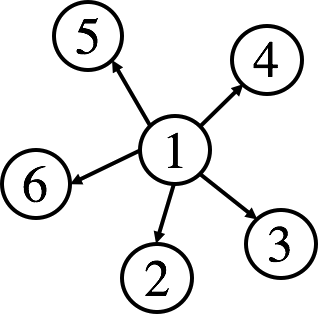
\includegraphics[width=0.14\textwidth,valign=c]{observcas}
		\vphantom{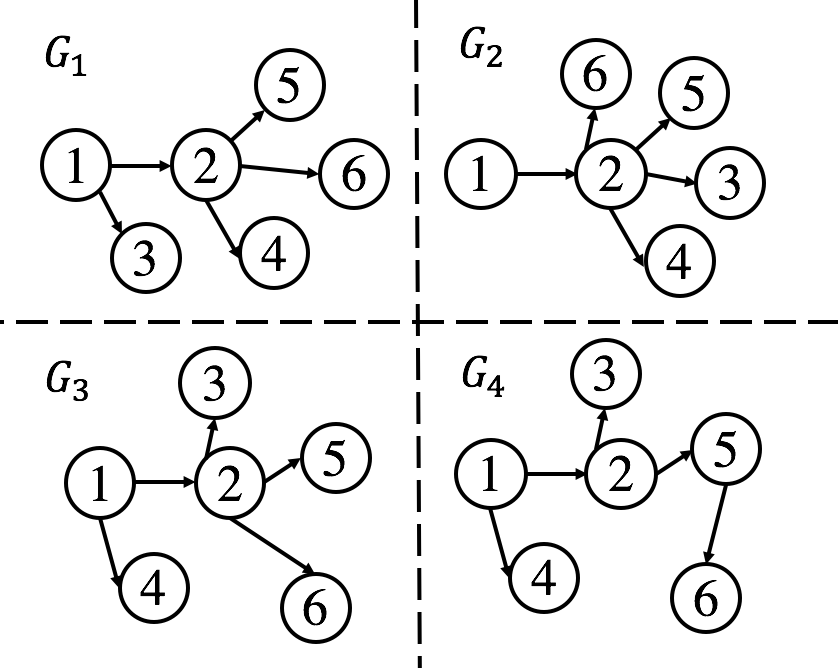
\includegraphics[height=\mywidth\textheight,valign=c]{somepossicas}}% MAR: this is here to keep the label at the same position as for the other figures.
		\label{fig:side:a}
	}
	\hspace{0.15cm}
	\subfloat[] {
		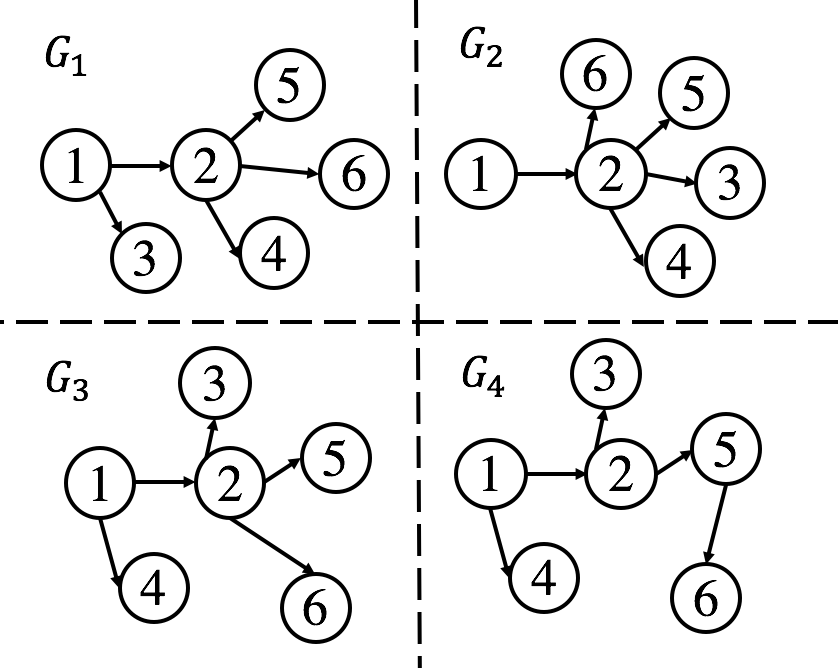
\includegraphics[height=\mywidth\textheight,valign=c]{somepossicas}
		\label{fig:side:b}
	}
	\hspace{0.15cm}
	\subfloat[] {
		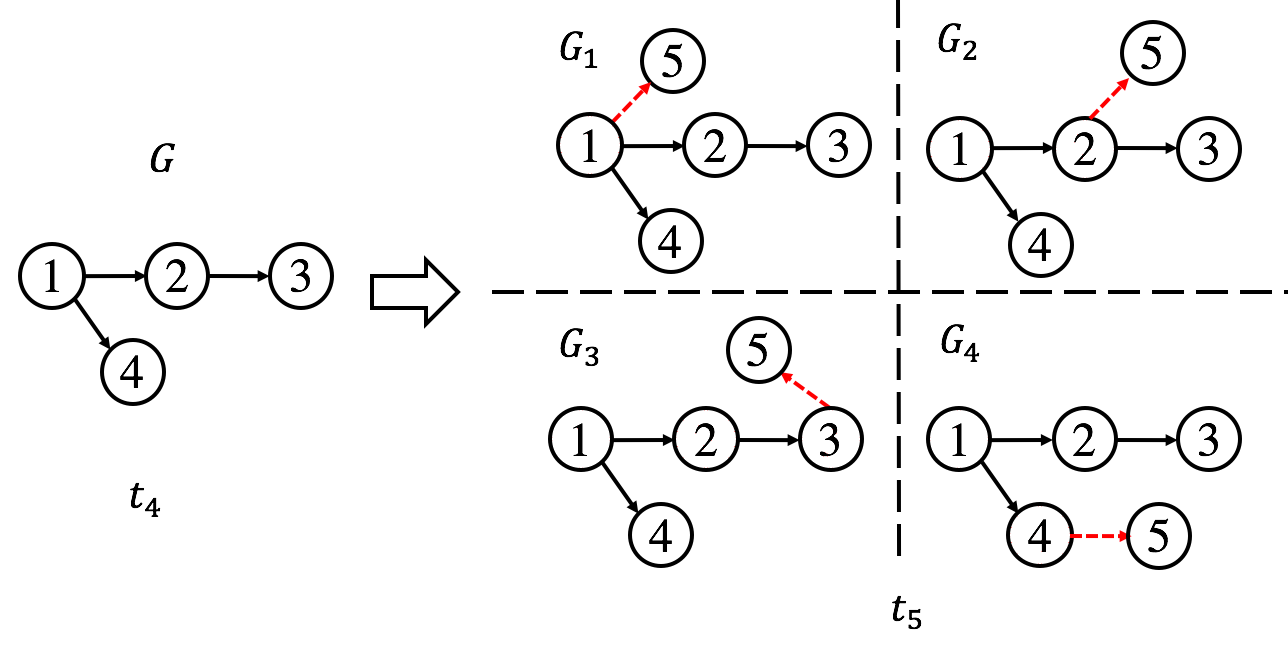
\includegraphics[height=\mywidth\textheight,valign=c]{gen_col}
		\label{fig:add-one-edge}
	}
	\caption{ 
		Modeling latent diffusions.
		\textbf{(a)} The schema of a retweet cascade as provided by the Twitter API, in which all retweets are attributed to the original tweet.
		\textbf{(b)} Four diffusion scenarios (out of 120 possible scenarios), associated with the retweet cascade in (a).
		\textbf{(c)} Intuition of the independent conditional model.
		A new node $v_5$ appears conditioned on one diffusion scenario $G$.
		Four new diffusion scenarios are generated as $v_5$ can attach to any of the existing nodes.
%		\hl{The influence of each of the nodes colored in red increases as $v_5$ attaches.}\verify{LX: unclear what ``increases'' refers to. suggest removing the red coloring and the sentence. i.e. this caption works equally well without the two highlighted sentences.}
	}
	\label{fig:holdout-ll}
%	\captionmoveup
\end{figure*}

%\subsection{Bot Presence and Behavior on Twitter During the 2016 U.S. presidential election}
\textbf{Bot presence and behavior on Twitter.}
\label{previousworkbots}
%
The `BotOrNot' Twitter bot detection API uses a Random Forest supervised machine learning classifier to calculate the likelihood of a given Twitter user being a bot, based on more than 1,000 features extracted from meta-data, patterns of activity, and tweet content (grouped into six main classes: user-based; friends; network; temporal; content and language; and sentiment) 
\cite{davisetal.16,varol.17}\footnote{See: \url{https://botometer.iuni.iu.edu/\#!/}}.
The bot scores are in the range $[0,1]$, where 0 (1) means the user is very unlikely (likely) to be a bot. 
%Evaluation against a publicly dataset of known Twitter bots demonstrated high accuracy and performance, and i
%It has been estimated that between 9\% and 15\% of active Twitter accounts are bots~\cite{varol.17}. 
BotOrNot was used to examine how socialbots affected political discussions on Twitter during the 2016 U.S. presidential election~\cite{FM7090}.
% collected data during all three presidential debates and the election period itself, resulting in a dataset of more than 20 million tweets by approximately 2.8 million unique user accounts authored between 16 September and 21 October 2016. The authors classified the top 50,000 accounts ranked by activity volume, accounting for 60\% of the overall conversation; accounts with a BotOrNot score higher than 0.5 were classed as bots and extrapolating from the sample to the entire population of accounts, 
They found that bots accounted for approximately 15 \% (400,000 accounts) of the Twitter population involved in election-related activity, and authored about 3.8 million (19 \%) tweets. 
However, \citet{FM7090} sampled the most active accounts, which could bias upwards their estimate of the presence of bots as activity volume is one of the features that is used by BotOrNot. 
They found that bots were just as effective as humans at \textit{attracting retweets} from humans. 
\citet{Woolley.2017} used BotOrNot to test 157,504 users randomly sampled from 1,798,127 Twitter users participating in election-related activity 
%during 1-11 Nov 
and found that over 10\% were bots. 
%with the same bot score threshold of 0.5
Here we use BotOrNot to classify \textit{all} 1.5 million users in our dataset to obtain a less biased approximation of their numbers and impact.
%rather than a random and/or purposive sample. 

Previous work has studied the political partisanship of Twitter bots.
\citet{Kollanyi.2016.presidentialdebate} analyzed candidate-oriented hashtag use during the 1st U.S. presidential debate and found that highly automated accounts (self-identified bots and/or accounts that post at least 50 times a day) were disproportionately pro-Trump.
% in terms of tweeting and retweeting  (e.g., \#MakeAmericaGreatAgain for Trump; \#ImWithHer for Clinton).
\citet{FM7090} also studied political partisanship by identifying five pro-Trump and four pro-Clinton hashtags and assigning users to a particular political faction.
% depending on which candidates hashtags were in the majority in the top 10 hashtags appearing in tweets by the user. 
The results suggested that both humans and bots were more pro-Trump in terms of hashtag partisanship.
%\TODO{@MAR}{In the paragraph below I have introduced some short statements that bridge the computer and social science parts of the paper, which also clarify or qualify our motivation for the study. Could you please check to make sure it's all technically correct?}
However, the above findings are limited to a comparison between humans and bots of frequency counts of tweets authored and retweets received, and they provide no insight into the importance of users in retweet diffusions. 
We overcome this limitation by modeling the latent structure of retweet diffusions and computing user influence over all possible scenarios.

%However, such findings concerning human and bot retweeting activity might be biased by the fact that the Twitter API does not allow direct observation of retweet cascades. 
%Analysis of retweets is effectively limited to frequency statistics of original tweets.
%and cannot determine whether a particular \textit{retweet} in the diffusion is the likely cause of a massive cascade.
%We overcome this limitation by modeling the latent structure of retweet diffusions and computing user influence over all possible scenarios.


% The working paper by \citet{Kollanyi.2016.presidentialdebate} analysed a sample of 4.5 million tweets collected around the time of the 1st U.S. presidential debate. A set of 52 election- and candidate-oriented hashtags (e.g., \#MakeAmericaGreatAgain for Trump; \#ImWithHer for Clinton) were used to collect the tweets, and it was found that `pro-Trump' tweets accounted for 39.1\%, while only  13.6\% were `pro-Clinton'. The authors also examined the behaviour of highly automated accounts (those that post at least 50 times a day), and they also identified accounts that included the term `bot' in the tag or profile description (i.e., self-disclosed bots). The authors found that 23.3\% of tweets were authored by these highly automated and/or bot accounts and they further contended that these accounts were pro-Trump, given these accounts authored about one third of the pro-Republican candidate tweets, compared to one fifth of the pro-Clinton tweets. 
% Whilst these findings are interesting, the heuristic used to classifying bots is potentially error-prone and does not appear to have been evaluated or justified with reference to existing approaches (e.g. BotOrNot) and the study did not provide enough detail to assess whether the particular set of hashtags chosen by the researchers could have introduced bias into the study.

%\textbf{Other related work.}
%Apart from influence of single nodes, influence between and of communities, i.e., clusters of nodes, is assessed with a Granger causality-based model~\cite{ICWSM1613006,Chikhaoui:2017:DCA:3127339.3070658}. Most work measures influence by quantitative approaches while some work warps up influence in a model for other tasks. \cite{ICWSM1613006} models news cycle's influence on Tweets by $\epsilon$-SVR (Support Vector Regression). By establishing the relationship between time and the tweets count, $\epsilon$-SVR implicitly contains News cycle's influence on tweets. 
%
%\subsection{Needs shortening and reducing}

%\TODO{MAR}{The following material is from Rui's thesis and unnecessary for this manuscript. They should be summarized in a 1-2 paragraps as ``somewhat related'' work. }
%\verify{There have been lots of work trying to modeling the self-exciting feature of different data such as tweets\cite{Mishra2016}, news articles \cite{Mishra2016}, Youtube videos \cite{Rizoiu2017} and maintenance data of the components of a general infusion pump \cite{taghipour2011trend}. In \cite{Mishra2016}, they use the Hawkes Point Process model with the Power-law triggering kernel in their method and consider various features including virality of tweet contents, user influence and memory decay in their triggering kernel. By using the L-BFGS algorithm to maximize the log-likelihood of cascades, they get optimal parameters of their model and predict the popularity of tweets and news articles. Tweets and news articles have a shared characteristic: the occurrence of a tweet or a new article is at a time point rather than roughly in a time interval. However, for the views of Youtube videos, we can only get the count of views in a specific time interval such as the last 24 hours so the time when a video is watched is unknown and Point-Process-based methods cannot effectively deal with these data any more. In order to deal with this problem, \cite{Rizoiu2017} propose event intensity, i.e., the expectation of the event rate over the event history. By minimizing the difference between event intensity of models and data, they train their model on views of videos in 90 days, which get a good prediction accuracy in predicting the popularity of these videos in the following 30 days. 

%Except modeling the self-exciting feature in the popular social media data, researchers also analyze the maintenance data in the engineering by modeling the self-exciting feature in these data\cite{taghipour2011trend}. The method in \cite{taghipour2011trend} exploit the Hawkes Point Process model with the Power-law kernel to model the self-exciting data and combines inferring the branching structure with optimizing model parameters by EM algorithm. In the E-step, they infer the branching structure and in the M-step, optimize parameters by the Newton-Raphson algorithm\cite{lange1995gradient}. The framework of our method is similar to \cite{taghipour2011trend} but we use L-BFGS\cite{liu1989limited} for optimization in the M-step of the EM algorithm. Newton-Raphson algorithm can deal with convex optimization but will be unstable to optimize non-convex functions. By theoretical analysis and experiments, we find our target function in the M-step of EM algorithm is non-convex and Newton-Raphson algorithm cannot effectively deal with it. 

%For uncovering the diffusion structure, there exist numerous different methods which can be separated into two classes: 1) NETINF and its extension\cite{gomez2010inferring,gomez2013structure,rodriguez2012submodular}; 2) the Hawkes Point Process and the mixture of Hawkes Point Processes\cite{simma2012modeling,cho2013latent,li2013dyadic,linderman2014discovering}. NETINF starts with independent points without edges and iteratively selects an edge which increase most significantly the log-likelihood of the network until the number of edges is equal to a target value. This method needs to calculate the probabilities of edges but select edges based on improvement of the log-likelihood so it is kind of different from distribution-based methods. 
%However, this kind of methods needs lots of cascades occurring on a retweet network to recover it precisely\cite{gomez2010inferring}. 
%The Hawkes Point Process model with the branching structure is actively used to uncover the diffusion structure, where hidden variables are introduced to represent the probabilities of the branching structure\cite{simma2012modeling,cho2013latent,li2013dyadic}. To calculate the hidden variables, people use EM algorithm to combine calculating hidden variables with optimizing model parameters. The mixture of Hawkes Point Processes model assumes multiple cascades influence each other and trys to model not only the branching structure in each cascade but also the influence between cascades \cite{li2013dyadic}. Notably, the frameworks of the mixture of Hawkes Point Processes models are similar to the frameworks of the single Hawkes Point Processes model.
%%}

%!TEX root = main.tex

%\secmoveup
\section{Estimating influence in retweet cascades}
\label{sec:user-influence}
%\secmoveup

%\verify{ \textbf{Comments from LX:}\\
%4/ 
%Sec 3.1 and 3.2 it seems better off to just call ``diffusion graph'' ``diffusion tree''. 
%this section should say that the tree respects temporal order,  it's unobserved / latent (and why we need to infer the tree)\\
%5/ 
%sec 3.2 path z, and $\phi$
%z should be defined as a sequence of nodes .. 
%Prob() is the probability of reaching $u_k$ from $u_i$, and $\phi$ would be the \textit{expected number of users reached} using a model of independent binomials to decide whether or not to take each hop in the path (instead of \textit{average number of reachable users} … unclear what it means)
%}

%\TODO{LX}{assuming the general motivation for inferring hidden tree + user influence was in intro. this sec first define cascade + tree + influence and proceed from there.}
%In Twitter, a {\em cascade} $C$ of size $n$ is defined as a series of messages $v_i$ sent by user $u_i$ at time $t_i$, i.e. $C=\{v_i(u_i, t_i)\}_{i=1}^n$.
%Here $v_1 = (u_1, t_1)$ is the initial message, and $v_1, \ldots, v_n$ with $t_1<\ldots<t_n$ are subsequent retweets or resposts of the initial message.

An {\em information cascade} $V$ of size $n$ is defined as a series of messages $v_i$ sent by user $u_i$ at time $t_i$, i.e. $V=\{v_i=(u_i, t_i)\}_{i=1:n}$.
Here $v_1 = (u_1, t_1)$ is the initial message, and $v_1, \ldots, v_n$ with $t_1<\ldots<t_n$ are subsequent reposts or relays of the initial message.
In the context of Twitter, the initial message is an original tweet and the subsequent messages are retweets of that original tweet (which by definition, are also tweets).
A latent retweet diffusion graph $G=(V,E)$ has the set of tweets as its vertexes $V$, and additional edges $E=\{(v_i, v_j)\}$ that represent that the $j^{th}$ tweet is a retweet of the $i^{th}$ tweet, and respects the temporal precedence $t_i<t_j$. 
Web data sources such as the Twitter API provide cascades, but not the
diffusion edges. 
Such missing data makes it challenging to measure a given user's contribution to the diffusion process.

%\TODO{LX}{now we need a precise definition of influence}
% now define influence

%\TODO{LX}{discussion: does $u$ feel more natural for denoting users in a graph than $v$ (vertex)?}


%\secmoveup
\subsection{Modeling latent diffusions}
\label{subsec:model-latent-diffusions}
%\secmoveup

\noindent\textbf{Diffusion scenarios.}
We focus on tree-structured diffusion graphs, i.e. each node $v_j$ has only one incoming link $(v_i, v_j)$, $i<j$. 
Denote the set of trees that are consistent with the temporal order in cascade $C$ as ${\cal G}$, we call each diffusion tree a \emph{diffusion scenario} $G \in {\cal G}$.
Fig.~\ref{fig:side:a} contains a cascade visualized as a star graph, attributing subsequent tweets to the first tweet at $t_1$.
Fig.~\ref{fig:side:b} shows four example diffusion scenarios consistent with this cascade.
The main challenge here is to estimate the influence of each user in the cascade, taking into account all possible diffusion trees.

\noindent\textbf{Probability of retweeting.}
%We define the probability of an edge $\mathds{P}(\{v_i, v_j\})$ as the likelihood that $u_j$ emitted tweet $v_j$ as a direct retweet of $v_i$.
For each tweet $v_j$, we model the probability of it being a direct descendant of each previous tweet in the same cascade as a weighted softmax function, defined by two main factors:
%% LX: the extra citations appear to be unecessary here
%as follows.
%In line with previous work~\cite{Mishra2016,Zhao2015,Shen2014}, we model two factors:
%\eat{in the likelihood of retweeting}:
firstly, users retweet \emph{fresh} content~\cite{Wu2007}.
We assume that the probability of retweeting decays exponentially with the time difference $t_j - t_i$;
secondly, users prefer to retweet locally influential users, known as preferential attachment~\cite{Barabasi2005,Rizoiu2017}.
We measure the local influence $m_i$ of a user $u_i$ using her number of followers~\cite{kwak2010twitter,Cha2010}.
%The second assumption is that user prefers retweet from a user who has a lot of followers. 
%The number of followers a user has often related to its number of retweet. 
%More followers, a user has more channels he can get to broadcast his tweet to others, which increasing the likelihood of seeing by other users~\cite{1,2}.
%So the probability of retweeting can be express in the following equation:
We quantify the probability that $v_j$ is a direct retweet of $v_i$ as:
\begin{equation} \label{eq:prob-edge-mt}
	p_{ij} = \frac{m_i e^{-r({t_j-t_i})}}{\sum_{k=1}^{j-1} m_k e^{-r({t_j-t_k})}}
\end{equation}
%This equation describe the probability that user $u_b$ retweet from user $u_a$ 
where 
%$t_a$ and $t_b$ represent the retweet time of $u_a$ and $u_b$ respectively;
$r$ is a hyper-parameter controlling the temporal decay. 
It is set to $r = 6.8 \times 10^{-4}$, tuned using linear search on a sample of 20 real retweet cascades (details in the supplement~\cite[annex~D]{supplemental}).
% and
%$m_i$ is the number of followers of user $u_i$ (the user of $v_i$).
%$e^{-r({t_{b}-t_{a}})}$ express the probability decrease in exponential.
%$G$ is one diffusion scenario which user $u_b$ is added to.
%The probability of a diffusion scenario is intimately linked to the probability of an edge.
%\TODO{LX}{this seems to be event rate not probability, i.e. not normalised}

%\secmoveup
\subsection{Tweet influence in a retweet cascade}
\label{subsec:user-influence-mt}
%\secmoveup

% \TODO{LX}{Is this a fair summary of the algorithm:\\ 
% * diffusion scenarios are the set of trees that are consistent with the cascade (order in time); \\
% * the algorithms marginalizes over all scenarios to estimate user influence; \\
% * the algorithm is efficient at $O(N^{XX})$ time; \\
% * it is non-obvious and potentially new because \ldots}

% assumptions + difficulties
We additionally assume retweets follow {\em independent conditional diffusions} within a cascade. 
%s
This is to say that conditioned on an existing partial cascade of $j-1$ retweets denoted as $V^{(j-1)}=\{v_k\}_{k=1}^{j-1}$ whose underlying diffusion scenario is $G^{(j-1)}$, the $j^{th}$ retweet is attributed to any of the $k=1,\ldots,j-1$ prior tweets according to Eq.~\ref{eq:prob-edge-mt}, and is independent of the diffusion scenario $G^{(j-1)}$. 
%s
For example, the $5^{th}$ tweet in the cascade will incur four valid diffusion trees for each of the diffusion scenarios for 4 tweets -- this is illustrated in Fig.~\ref{fig:add-one-edge}. 
%s
This simplifying assumption is reasonable, as it indicates that each user $j$ makes up his/her own mind about whom to retweet, and that the history of retweets is available to user $j$ (as is true in the current user interface of Twitter).
%s
It is easy to see that under this model, the total number of valid diffusion trees for a 5-tweet cascade is $1\cdot 2\cdot 3\cdot 4=24$, and that for a cascade with $n$ tweets is $(n-1)!$.

The goal for influence estimation for each cascade is to compute the contribution $\varphi(v_i)$ of each tweet $v_i$ {\em averaging} over all independent conditional diffusion trees consistent with cascade $V$ and with edge probabilities prescribed by Eq.~\ref{eq:prob-edge-mt}. 
%s
Enumerating all valid trees and averaging is clearly computationally intractable, but the illustration in Fig.~\ref{fig:add-one-edge} lends itself to a recursive algorithm. 

\textbf{Tractable tweet influence computation}
We introduce the \emph{pair-wise influence score} $m_{ij}$ which measures the influence of $v_i$ over $v_j$.
$v_i$ can influence $v_j$ both directly when $v_j$ is a retweet of $v_i$, and indirectly when a path exists from $v_i$ to $v_j$ in the underlying diffusion scenario.
Let $v_k$ be a tweet on the path from $v_i$ to $v_j$ ($i < k < j$) so that $v_j$ is a direct retweet of $v_k$.
$m_{ik}$ can be computed at the $k^{th}$ recursion step and it measures the influence of $v_i$ over $v_k$ over all possible paths starting with $v_i$ and ending with $v_k$.
Given the above independent diffusions assumption, the $m_{ij}$ can be computed using $m_{ik}$ to which we add the edge $(v_k, v_j)$.
User $u_j$ can chose to retweet any of the previous tweets with probability $p_{kj}, k < j$, therefore we further weight the contribution through $v_k$ using $p_{ij}$.
We consider that a tweet has a unit influence over itself ($m_{ii} = 1$).
Finally, we obtain that:
\begin{equation} \label{eq:Mij-mt}
m_{ij} =
\left\{
\begin{array}{ll}
	\sum^{j-1}_{k=i} m_{ik}p_{kj}^2 &,i < j \\
	1 & ,i = j \\
	0 & ,i > j.
\end{array}
\right.
\end{equation}

Naturally, $\varphi(v_i)$ the total influence of node $v_i$ is the sum of $m_{ij}, j > i$ the pair-wise influence score of $v_i$ over all subsequent nodes $v_j$. 
The recursive algorithm has three steps. 
\begin{enumerate}
	\item {\bf Initialization.} $m_{ij}=0$ for $i, j=1,\ldots,n, j \neq i$, and $m_{ii} = 1$ for $i=1,\ldots,n$;
	\item {\bf Recursion.} For $j=2, \ldots, n$;
	\begin{enumerate}
		\item For $k=1, \ldots, j-1$, compute $p_{kj}$ using Eq.~\eqref{eq:prob-edge-mt};
		\item For $i=1, \ldots, j-1$, $m_{ij} = \sum_{k=i}^{j-1} m_{ik}p_{kj}^2$;
	\end{enumerate}
	\item {\bf Termination.} Output $\varphi(v_i)= \sum_{k=i+1}^n m_{ik}$, for $i=1,\ldots,n$. 
\end{enumerate}

We exemplify this algorithm on a 3-tweet toy example. 
%s
%\oldversion{\hl{TO BE UPDATED}
Consider the cascade $\{v_1, v_2, v_3\}$.
When the first tweet $v_1$ arrives, we have $m_{11} = 1$ by definition (see Eq.~\eqref{eq:Mij-mt}).
%
% and denote $m_{ij}$ as a vector of the m-score values for each node for the first tweet (i.e., $v_1$). 
%s
%This is a all-zero vector by definition, as there are no retweets yet. 
%s
After the arrival of the second tweet, which must be retweeting the first, we have 
$m_{12}= m_{11} p^2_{12}=1$, and $m_{22} = 1$ by definition.
%to account for the influence of $v_1$, 
%and $\phi^{(2)}_2=\phi^{(2)}_3=0$. 
%s 
The third tweet can be a retweet of the first or the second, therefore we obtain: 
\begin{align*}
	m_{13} =& m_{11} p^2_{13} + m_{12} p^2_{23} \; ;\\
	m_{23} =& m_{22} p^2_{23} \; ;\\
	m_{33} =& 1 \;.
\end{align*}
The second term of $m_{13}$ accounts for the indirect influence of $v_1$ over $v_3$ through $v_2$.
%$\phi^{(3)}_1$ has three terms, the first term denotes the influence node $v_1$ already had on $v_2$, the second term denotes the direct influence of $v_1$ to $v_3$ had node 3 is a retweet of node 1. 
%The influence of $v_3$ itself is still zero: $\phi^{(3)}_3=0$. Moreover, 
This is the final step for a 3-node cascade. 
%The algorithm outputs $[\phi_i]_{i=1:3}=[\phi^{(3)}_i]_{i=1:3}$. 
%}

%As a sanity check, we can see that $\sum_{i=1}^n \varphi(v_i) = \sum_{j=1}^n \sum_{i=1}^{j-1} \Pd ((v_i,v_j)) = n-1$. In other words, the total influence across all nodes in a cascade of size $n$ is equal to $n-1$, or the number of retweets in this cascade. 
%In addition, the recursion above permits an in-place implementation, i.e., we incrementally update $\varphi(v_i)$ in step 2, and do not need to keep the intermediate influence values $\phi^{(k)}(v_i)$.
The computational complexity of this algorithm is $O(n^3)$.
There are $n$ recursion steps, and calculating $p_{ij}$ at sub-step (a) needs $O(n)$ units of computation, and sub-step (b) takes $O(n^2)$ steps.
In real cascades containing 1000 tweets, the above algorithm finishes in 34 seconds on a PC.
For more details and examples, see the online supplement~\cite[annex~B]{supplemental}.

%\oldversion{
%\textbf{Tweet influence over one diffusion scenario.}
%Let $z(v_i, v_k) \in G$ be a path in the diffusion scenario $G$ -- i.e a sequence of nodes which starts with $v_i$ and ends with $v_k$.
%$\mathds{P}(z(v_i, v_k))$ is the probability of reaching $v_k$ from $v_i$.
%We define $\varphi(v_i | G)$ the influence of $v_i$ in the scenario $G$ as the expected number of users reached from $v_i$ using a model of independent binomials to decide whether or not to take each hop in each path that starts with $v_i$.
%Formally:
%\begin{align}
%	\varphi(v_i|G) 	&= \mathds{E} \left[ \sum_{v_k \in V(G)} \mathds{1} \left\lbrace z(v_i,v_k|G) \right\rbrace \right] \nonumber \\
%					&= \sum_{v_k \in V(G)} \mathds{E}\bigg[\mathds{1} \left\lbrace z(v_i,v_k|G) \right\rbrace \bigg] \nonumber \\
%					&= \sum_{v_k \in V(G)} \mathds{P}(z(v_i,v_k|G)) \nonumber \\
%					&= \sum_{v_k \in V(G)} \prod_{(v_a, v_b) \in z(v_i, v_k)} \mathds{P}\big((v_a, v_b)\big) \label{eq:infl-in-a-scenario-mt}
%\end{align}
%where $\mathds{1} \left\lbrace z(v_i,v_k|G) \right\rbrace$ is a function that takes the value 1 when the path from $v_i$ to $v_k$ exists in $G$, and 0 otherwise.
%
%\textbf{Tweet influence over a retweet cascade.}
%
%
%We define $\varphi(v_i)$ the influence of $v_i$ over all valid diffusion scenarios $\cal G$:
%\begin{align}
%	\varphi(v_i) 	&= \sum_{G\in{\cal G}} \mathds{P}(G) \varphi(v_i|G) \nonumber \\
%				&= \sum_{G\in{\cal G}} \mathds{P}(G) \sum_{v_k \in V(G)} \mathds{P}\big( z(v_i,v_k|G) \big) \label{eq:brute-user-infl-mt}
%\end{align}
%Under the assumption that retweeting events (i.e. edges) occur independently one from another, the probability of a diffusion scenario is:
%\begin{equation} \label{eq:prob-scenario-mt}
%	\mathds{P}(G) = \prod_{(v_a, v_b) \in E} \mathds{P}\big((v_a, v_b)\big)
%\end{equation}
%
%It is intractable to directly evaluate Eq.~\eqref{eq:brute-user-infl-mt} (together with Eq.~\eqref{eq:infl-in-a-scenario-mt} and~\eqref{eq:prob-scenario-mt}), particularly due to the factorial number of diffusion scenarios in $\cal G$ (as shown in the online supplement~\cite[annex~A]{supplemental}).
%%\ref{si-sec:infl-derivation}
%For example, there are $10^{156}$ diffusion scenarios for a cascade of 100 retweets.
%We develop, in the next section, an efficient \eat{linear time} algorithm to compute the influence of all tweets\eat{in a retweet cascade}.
%
%%\verify{RJA comment: This might be basic question but is the probability threshold 0.5? i.e. estimated prob needs to be greater than 0.5 for there to be edge from from user i to j in retweet cascade?}
%%% MAR: not really. We don't make a decision based on probabilities, but we work in probability space.
%%RJA: OK I think I get it now.
%
%%\secmoveup
%\subsection{Tractable tweet influence computation}
%\label{subsec:casin-algo}
%%\secmoveup
%
%The key observation for a tractable computation of Eq.~\eqref{eq:brute-user-infl-mt} is that tweets $v_k$ are added sequentially at time $t_k$, to each diffusion scenario constructed at time $t_{k-1}$.
%Adding $v_k$ to a diffusion scenario $G$ has two effects.
%First, $k-1$ new diffusion scenarios are generated, as $v_k$ can attach to any of the existing $k-1$ nodes.
%Second, $v_k$ contributes only once to the tweet influence of each tweet that is found on the branch it attaches to and it does not make any other contributions at times $t > t_k$.
%This process is exemplified in Fig.~\ref{fig:add-one-edge}.
%Node $v_5$ is added to a given diffusion scenario, generating 4 new diffusion scenarios at time $t_5$.
%The nodes colored in red see their influence increase as a result of adding $v_5$.
%%We color in red the nodes whose influence increases as a result of adding node $v_5$.
%This allows to compute tweet influence incrementally, by updating $\varphi(v_i), i < k$ at each time $t_k$.
%We denote by $\varphi^k(v_i)$ the value of tweet influence of $v_i$ after adding node $v_k$.
%Thus, we only keep track of how tweet influence increases as nodes attach and we do not need to construct all diffusion scenarios.
%
%We define $M_{ik}$ as the contribution of $v_k$ to the tweet influence of $v_i$, over all possible diffusion scenarios.
%It can be shown that the influence of $v_i$ increases at time $t_k$ by $M_{ik}$:
%\begin{equation} \label{eq:iter-computation}
%	\varphi^k(v_i) = \varphi^{k-1}(v_i) + M_{ik},
%\end{equation}
%\begin{equation} \label{eq:Mij-mt}
%\text{ where } M_{ik} =
%\left\{
%\begin{array}{ll}
%	\sum^{k-1}_{j=1}M_{ij}\mathds{P}^2 \big( (v_j, v_k) \big) &,i < k \\
%	1 & ,i = k \\
%	0 & ,i > k.
%\end{array}
%\right.
%\end{equation} 
%See the online supplement~\cite[annex~B]{supplemental} for the complete derivation from Eq.~\eqref{eq:brute-user-infl-mt} to Eq.~\eqref{eq:iter-computation} and~\eqref{eq:Mij-mt}. %\ref{si-sec:efficient-algo}
%
%%\verify{RJA comment: Absolutely not suggesting any change to the above [no time anyway!] but I'm just wondering why a user is allowed to influence herself? I thought it would be $M_{ik} =0, i \geq k$. Doesn't have any impact on the comparative results, of course}
%%% MAR: we need it for the math. For comparative results, we plot percentiles anyway, so +1 simply puts everyone higher, but does not change order.
%
%\textbf{Recursive computation of tweet influence.}
%$M_{ik}$ can be alternatively interpreted as the influence of tweet $v_i$ over $v_k$.
%Consequently, we can compute $\varphi^k(v_i)$ the total influence of $v_i$ as the sum of 
%the individual influences of $v_i$ over each of the other nodes in the diffusion.
%% influence that $v_i$ has over all the other nodes in the cascade.
%This can be recursively computed as:
%\begin{align*}
%	\varphi^k(v_i) &= \varphi^{k-1}(v_i) + M_{ik} \nonumber \\
%				   &= \varphi^{k-2}(v_i) + M_{i(k-1)} + M_{ik} = \ldots = \sum_{j=1}^k M_{ij}. 
%\end{align*}
%
%\begin{algorithm}[tbp]
%\color{gray}
%  \caption{Compute influence matrix $M$, \hl{LX: $\Pd_{ij}^2$ and matrix $M$ are unclear}}
%  \label{alg1}
%  \begin{algorithmic}
%  \REQUIRE A set of $n$ retweets $\{ v_i = (m_i, t_i) | i = 1,\dots,n\}$
%  \REQUIRE Parameter $r$ -- temporal decay.
%  \ENSURE influence matrix $M$
%
%  \STATE Initialize matrix $P = [ P_{ij} = 0, \forall i, j = 1,\dots,n]$
%  \STATE Initialize matrix $M = [ M_{ij} = 0, \forall i, j = 1,\dots,n]$
%  \STATE $M_{11} = 1$
%
%  \FOR{$i=1$ \TO $n$}
%  		\FOR{$j=i$ \TO $n$}
%  			\STATE $P_{ij} = m_i e^{-r({t_j-t_i})}$
%  		\ENDFOR
%  \ENDFOR
%  %\STATE \hl{column normalize $P_{ij}$}
%  \STATE \rvx{$P_{ij} \leftarrow P_{ij}/(\sum_i P_{ij})$}
%  \STATE \hl{$P_{ij} = P_{ij} \cdot P_{ij}$ (element-wise multiplication)}
%  
%  \FOR{$j=2$ \TO $n$} {
%		\STATE \hl{$M_{[1..j-1, j]} = M_{[1..j-1, 1..j-1]} \times P_{[1:j-1,j]}$}
%		\STATE $M_{jj} = 1$	
%  }\ENDFOR
%
%  \end{algorithmic}
%  \label{alg:casin}
%\end{algorithm}
%
%\textbf{Computational complexity for estimating influence.}
%The scalable influence computation algorithm shown in Algorithm~\ref{alg:casin} uses two matrices:
%matrix $P = [ P_{ij} ]$, with $P_{ij} = \mathds{P}^2 \big( (v_i, v_j) \big)$ and matrix $M = [ M_{ij} ]$.
%It computes each column of $M$ sequentially, using Eq.~\eqref{eq:Mij-mt}.
%%Assuming that matrix multiplications are executed in $O(1)$,
%%The computation of matrix $M$ finishes after $n$ steps (or rows??). 
%Recursively computing each column in $M$ takes $O(n^2)$ multiplications/additions, the total computations complexity is $O(n^3)$. 
%In real cascades containing 1000 tweets, the above algorithm finishes in 34 seconds on a PC.
%%, where $n$ is the total number of retweets in the retweet cascade.
%For more details and examples, see the online supplement~\cite[annex~B]{supplemental}.
%%\ref{si-sec:efficient-algo}
%\eat{
%%%LX: moved the following info to Sec 3.1, as it doesn't describe "Computational complexity"
%Throughout the experiments in Sec.~\ref{sec:evaluation-influence}
% and~\ref{sec:results-findings}, we set the temporal decay hyper-parameter defined in Eq~\eqref{eq:prob-edge-mt} to $r = 6.8 \times 10^{-4}$, tuned using linear search on a sample of 20 real retweet diffusions (details in the online supplement~\cite[annex~D]{supplemental}). %\ref{si-sec:choose-temp-decay}
% }
%
%}

\subsection{Computing influence of a user}
\label{subsec:user-influence-measure}

Given $\mathcal{T}(u)$ -- the set of tweets authored by user $u$ --, we define the user influence of $u$ as the mean tweet influence of tweets $v \in \mathcal{T}(u)$:
\begin{equation} \label{eq:user-infl-casin}
	\varphi(u) = \frac{\sum_{v \in \mathcal{T}(u)} \varphi(v)}{|\mathcal{T}(u)|}, \mathcal{T}(u) = \{ v | u_v = u\}
\end{equation}
To account for the skewed distribution of user influence, we mostly use the normalization --  percentiles with a value of 1 for the most influential user our dataset and 0 for the least influential -- denoted $\varphi(u) \%$ .
%To account for the skewed distribution of user influence, the results presented in Sec.~\ref{sec:evaluation-influence} and~\ref{sec:results-findings} use the percentile normalized values of user influence with a value of 1 for the most influential user our dataset and 0 for the least influential.

%!TEX root = main.tex

\section{Dataset and measures of political behavior}
\label{sec:four-measures}

In this section, we first describe the \debate dataset that we collected during the 1st U.S. presidential debate.
Next, we introduce three measures for analyzing the political behavior of users who were active on Twitter during the debate.
In Sec.~\ref{subsec:political-polarization-measures}, we introduce \emph{political polarization} $\mathcal{P}$ and \emph{political engagement} $\mathcal{E}$.
In Sec.~\ref{subsec:bot-detection} we introduce the \emph{botness score} $\zeta$ and we describe how we construct the reference bot and human populations.
%Finally, in Sec.~\ref{subsec:user-influence-measure} we compute the user influence $\varphi$ based on all retweet cascades in \debate.

%\subsection{The \debate dataset}
%\label{subsec:debatenight-construction}

\textbf{The \debate dataset}
contains Twitter discussions that occurred during the 1st 2016 U.S presidential debate between Hillary Clinton and Donald Trump.
Using the Twitter Firehose API\footnote{Via the Uberlink Twitter Analytics Service.}, we collected all the tweets (including retweets) that were authored during the two hour period from 8.45pm to 10.45pm EDT, on 26 September 2016, and which contain at least one of the hashtags: \texttt{\#DebateNight}, \texttt{\#Debates2016}, \texttt{\#election2016}, \texttt{\#HillaryClinton}, \texttt{\#Debates}, \texttt{\#Hillary2016}, \texttt{\#DonaldTrump} and \texttt{\#Trump2016}.
The time range includes the 90 minutes of the presidential debate, as well as 15 minutes before and 15 minutes after the debate.
The resulting dataset contains 6,498,818 tweets, emitted by 1,451,388 twitter users.
For each user, the Twitter API provides aggregate information such as the number of followers, the total number (over the lifetime of the user) of emitted tweets, authored retweets, and favorites.
For individual tweets, the API provides the timestamp and, if it is a retweet, the original tweet that started the retweet cascade.
The \debate dataset contains 200,191 retweet diffusions of size 3 and larger.
%Using this information, we \rev{used the approach described in Section~\ref{sec:user-influence} to reconstruct} 200,191 complete retweet cascades\footnote{We make sure that no retweets are missing from cascades by checking the \texttt{retweets\_count} field provided by Twitter API.} of size at least 3.
%As the \#DebateNight hashtag accounts for over half of the tweets, we refer to our data as the "\#DebateNight dataset".

\subsection{Political polarization $\mathcal{P}$ and engagement $\mathcal{E}$}
\label{subsec:political-polarization-measures}

%!TEX root = main.tex

%% MAR: the wordclouds were obtained using "https://wordart.com/create"
\begin{figure}[tbp]
	\centering
	\newcommand\mywidth{0.45}
	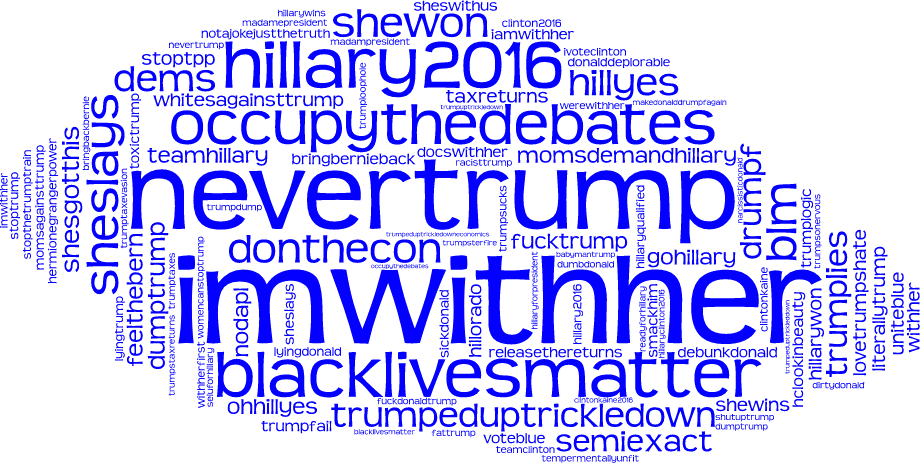
\includegraphics[width=\mywidth\textwidth]{democrat-2} %% also good democrat-4
	\vspace{0.1cm}\\
	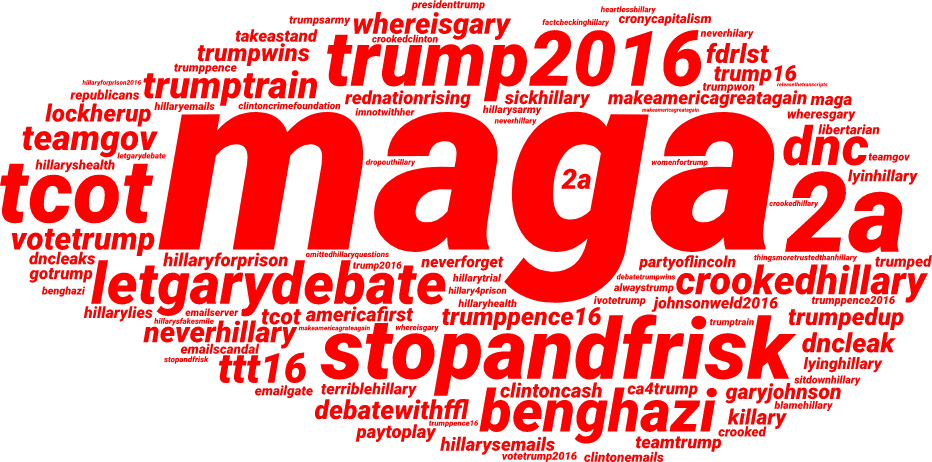
\includegraphics[width=\mywidth\textwidth]{republican-1}
	\caption{
		Wordclouds of partisan hashtags in \debate: Democrat \textbf{(top)} and Republican \textbf{(bottom)}.
		Hashtags sizes are scaled by their frequency.
	}
	\label{fig:wordclouds}
%	\captionmoveup
\end{figure}

%\TODO{@TG}{This paragraph does not make it clear that we ONLY chose ``clearly partisan'' hashtags, and not generally Democrat- or Republican-leaning hashtags.
%This should address inevitable questions about why only 1k tweets have both, and also RJA's remark in Sec 6 about why so little users in the middle of Fig. 4a.
%See text in purple here below.}

\textbf{Protocol.}
Content analysis~\cite{kimkuljis2010} was used to code the 1000 most frequently occurring hashtags according to their political polarity. More specifically, we used 
Directed Content Analysis~\cite{hsieh-shannon-2005} to contextually analyse hashtags and code them according to their political polarity (or not, denoted as `neutral' and subsequently excluded from analysis). 
This approach has been used in previous work to study hashtags on Twitter in a manner that is valid, reliable and replicable~\cite{small-2011}. 
There were two previous studies of Twitter activity during the 2016 U.S. presidential election that informed the development of our coding schema. 
Firstly, \citet{FM7090} devised a binary classification scheme that attributed political partisanship to a small set of key hashtags as either `Trump-supporting' (\#donaldtrump, \#trump2016, \#neverhillary, \#trumppence16, \#trump) or `Clinton-supporting' (\#hillaryclinton, \#imwithher, \#nevertrump, \#hillary). 
Secondly, in studying Twitter activity during the 1st U.S. presidential debate, \citet{Kollanyi.2016.presidentialdebate} developed a coding schema that categorized tweets into seven categories based on the hashtags that occurred within the tweet. 
However, the authors found that three `exclusive' categories (`Pro-Trump', `Pro-Clinton', and `Neutral') accounted for the majority (88.5\%) of observations. 

Given the findings of previous research, we developed a code book with three categories: `Pro-Trump', `Pro-Clinton', and `Neutral'. 
To ensure that hashtags were analyzed within context, our content analysis methodology focussed on three units of analysis (following the approach developed by~\citet{small-2011}). 
The first is hashtags, comprised of a set of the 1000 most frequently occurring hashtags over all tweets in our dataset. 
The second unit of analysis was individual tweets that contained these hashtags. 
In order to gain a more nuanced and `situated' interpretation of hashtag usage, for each hashtag we referred to a small random sample of tweets in our dataset that contained each given hashtag. 
In some instances the polarity (or neutrality) was clear and/or already determined from previous studies, which helped to speed up the analysis of tweets. 
The third unit of analysis was user profiles, which we referred to in situations where the polarity or neutrality of a given hashtag was unclear from the context of tweet analysis. 
For example, \#partyoflincoln was used by both Republican and Democrat Twitter users, but an analysis of both tweets and user profiles indicated that this hashtag was \textit{predominantly} used by Pro-Trump supporters to positively align the Republican Party with the renowned historical figure of President Abraham Lincoln, who was a Republican. 
The content analysis resulted in a subset of 93 pro-Democrat and 86 pro-Republican hashtags (see the wordcloud visualization in Fig.~\ref{fig:wordclouds}), whilst the remaining `neutral' hashtags were subsequently excluded from further analysis.
The resulting partisan hashtag list contains hashtags indicating either strong support for a candidate (e.g., \texttt{\#imwithher} for Clinton and \texttt{\#trump2016} for Trump), or opposition and/or antagonism (e.g., \texttt{\#nevertrump} and \texttt{\#crookedhillary}).
The complete list of partisan hashtags is publicly available in the Github repository.

%% MAR: this is the old shortened version of the protocol (used in submission)
%We extracted the 1000 most frequent hashtags in our dataset. 
%Using a content analysis approach~\cite{kimkuljis2010}, we coded each hashtag into two categories: Democrat and Republican. 
%Hashtags that did not have a clear political polarity were not labeled and thus excluded from analysis. 
%Our coding methodology is similar to previous work~\cite{Kollanyi.2016.presidentialdebate,FM7090},
%%This follows a similar coding methodology to related studies 
%%although rather than starting with a preconceived set of partisan hashtags we derived these from the data. 
%with the difference that we extract candidate hashtags from the data instead of using a predefined set of partisan hashtags.
%Fig.~\ref{fig:wordclouds} presents the wordclouds of the most frequent partisan hashtags, for Democrats (top) and Republicans (bottom).
%We chose hashtags indicating either strong support for a candidate (e.g., \texttt{\#imwithher} for Clinton and \texttt{\#trump2016} for Trump), or opposition and/or antagonism (e.g., \texttt{\#nevertrump} and \texttt{\#crookedhillary}). 
%\rev{Hashtags were coded in the context of the political discussion.
%More details on the coding protocol can be found in the online supplement~\cite[annex~F]{supplemental}.}
%This results in 93 Democrat and 86 Republican hashtags.
%\rev{The list of partisan hashtags is publicly available in the Github repository.}

\textbf{Two measures of political behavior.}
We identify 65,031 tweets in \debate that contain at least one partisan hashtag (i.e., one of hashtags in the reference set of partisan hashtags constructed earlier).
1,917 tweets contain partisan hashtags with both polarities: these are mostly negative tweets towards both candidates (e.g., ``Let's Get READY TO RUMBLE AND TELL LIES. \#nevertrump \#neverhillary \#Obama'') or hashtag spam.
We count the number of occurrences of partisan hashtags for each user, and we detect a set of 46,906 politically engaged users that have used at least one partisan hashtag.
Each politically engaged user $u_i$ has two counts: $dem_i$ the number of Democrat hashtags that $u_i$ used, and $rep_i$ the number of Republican hashtags.
We measure the \emph{political polarization} as the normalized difference between the number of Republican and Democrat hashtags used:
\begin{equation}
	\mathcal{P}(u_i) = \frac{rep_i - dem_i}{rep_i + dem_i}.
\end{equation}
$\mathcal{P}(u_i)$ takes values between $-1$ (if $u_i$ emitted only Democrat partisan hashtags) and $1$ ($u_i$ emitted only Republican hashtags).
We threshold the political polarization to construct a population of Democrat users with $\mathcal{P}(u) \leq -0.4$ and Republican users with $\mathcal{P}(u) \geq 0.4$.
In the set of politically engaged users, there are 21,711 Democrat users, 22,644 Republican users and 2,551 users with no polarization ($\mathcal{P}(u) \in (-0.4, 0.4)$).
%
We measure the \emph{political engagement} of users using the total volume of partisan hashtags included in their tweets $\mathcal{E}(u_i) = rep_i + dem_i$.

\subsection{Botness score $\zeta$ and bot detection}
\label{subsec:bot-detection}

%% MAR: cutting down on the motivation, should be in intro, not here.
%A key problem is how to classify user accounts who participated in \#DebateNight into those who are human versus those who are bots and/or `highly automated' \cite{Kollanyi.2016.presidentialdebate}. The large of number of users in our dataset (over 1.5 million) meant that manual human classification was not possible within a reasonable time-frame and resources\footnote{For instance, if each user took 30 seconds to manually annotate, it would take over 1.5 years for a researcher working 24 hours a day.}. Therefore, we used a state-of-the-art bot detection system known as `BotOrNot', discussed previously in Sec.~\ref{previousworkbots}.

\textbf{Detecting automated bots.}
%Using the BotOrNot API, we classified each of the 1,451,388 users in our dataset to extract their bot scores. 
We use the BotOrNot~\cite{davisetal.16} API to measure the likelihood of a user being a bot for each of the 1,451,388 users in the \debate dataset.
Given a user $u$, the API returns the botness score $\zeta(u) \in [0, 1]$ (with 0 being likely human, and 1 likely non-human).
%Next, we determined a threshold value to decide whether a user is a bot or not. 
%The BotOrNot authors indicate that this is a non-trivial problem due to the varying levels of sophistication of bots and the fact that bots are continuously changing and being modified to thwart detection. 
%As a starting point, we chose a threshold value of 0.5, which the authors indicate provided an overall classification accuracy of 86\% through their cross-validation process (Varol et al., 2017: 283), and is also a threshold used in previous studies \cite{FM7090,Woolley.2017}. 
%In this way, if a user scored above 0.5 then they were classified as a bot. 
Previous work~\cite{varol.17,FM7090,Woolley.2017} use a botness threshold of $0.5$ to detect socialbots.
However, we manually checked a random sample of 100 users with $\zeta(u) > 0.5$ and we found several human accounts being classified as bots.
A threshold of 0.6 decreases mis-classification by $3\%$.
%whilst raising the threshold to 0.6 provided more accurate results. 
%we therefore employ a threshold of $0.6$ to differentiate bot-like accounts.
%We observed that a number of organizational accounts were misclassified as bots. 
It has been previously reported by \citet{varol.17} that organizational accounts have high botness scores.
%This issue relating to misclassification of organizational accounts was reported by \cite[p. 2]{varol.17}. 
This however is not a concern in this work, as we aim to detect 
%However, this was not a concern as we were not only interested in bots but also 
`highly automated' accounts that behave in a non-human way. 
We chose to use a threshold of $0.6$ to construct the \Bot population in light of the more encompassing notion of account \emph{automation}. 
%On the other hand, manual analysis of a small random sample of `human' accounts (with scores $<= 0.6$) showed that setting a threshold of 0.2 allowed us to classify accounts as almost certainly human (operated by a single living individual). 
%We then converted the bot scores over all users into a dichotomous variable, i.e., 0 for human; 1 for bot) and applied it to our network as a node attribute for further analysis.

%!TEX root = main.tex

%% latex table generated in R 3.4.0 by xtable 1.8-2 package
%% Thu Nov 30 17:07:53 2017
%\begin{table}[tb]
%	\renewcommand{\cellalign}{cr}
%	\scriptsize
%%	\fontsize{6.5pt}%{10.0pt}
%%	\selectfont
%	\setlength{\tabcolsep}{5pt}
%	\centering
%	\caption{
%		Tabulating population volumes and percentages of politically polarized users over four populations: \Protected, \Human, \Suspended and \Bot.
%%		Retrieving botness score failed for 4,822 users.
%	}
%	\begin{tabular}{rr|rrr|rr}
%		\toprule
%			& All & Polarized & Dem. & Rep. & Dem. \% & Rep. \% \\ 
%  		\midrule
%			All & 1,451,388 & 44,299 & 21,676 & 22,623 & 48.93\% & 51.07\% \\ 
%  			\Protected & 45,316 & 1,245 & 585 & 660 & 46.99\% & 53.01\% \\ 
%			\makecell{\Human\\($\zeta \leq 0.2$)} & 499,822 & 11,972 & 5,376 & 6,596 & 44.90\% & 55.10\% \\ 
%  			\Suspended & 10,162 & 265 & 111 & 154 & 41.89\% & 58.11\% \\ 
%  			\makecell{\Bot\\($\zeta \geq 0.6$)} & 17,561 & 435 & 185 & 250 & 42.53\% & 57.47\% \\ 
%   		\bottomrule
%	\end{tabular}
%	\label{tab:populations-effectives}
%	\captionmoveup
%\end{table}

% MAR: one idea is to transpose this table, because the scriptsize above is ugly.
%		But extra work is required.
% latex table generated in R 3.4.0 by xtable 1.8-2 package
% Thu Nov 30 17:07:53 2017
\begin{table}[tb]
	\renewcommand{\cellalign}{cr}
	\small
	\setlength{\tabcolsep}{4pt}
	\centering
	\caption{
		Tabulating population volumes and percentages of politically polarized users over four populations: \Protected, \Human, \Suspended and \Bot.
%		Retrieving botness score failed for 4,822 users.
	}
	\begin{tabular}{rrrrrr}
		\toprule
			& All & \texttt{Prot.} & \Human & \texttt{Susp.} & \Bot \\
  		\midrule		
			All & 1,451,388 & 45,316 & 499,822 & 10,162 & 17,561 \\
			Polarized & 44,299 & 1,245 & 11,972 & 265 & 435 \\
			Democrat & 21,676 & 585 & 5,376 & 111 & 185 \\
			Republican & 22,623 & 660 & 6,596 & 154 & 250 \\
		\midrule
			Dem. \% & 48.93\% & 46.99\% & 44.90\% & 41.89\% & 42.53\%\\
			Rep. \% & 51.07\% & 53.01\% & 55.10\% & 58.11\% & 57.47\%\\ 
   		\bottomrule
	\end{tabular}
	\label{tab:populations-effectives}
%	\captionmoveup
\end{table}

\textbf{Four reference populations.}
In addition to the \Bot population, we construct three additional reference populations:
%, based on the ``BotOrNot'' API \cite{varol.17}. \emph{Bot} have a bot score $\ge 0.6$; users in this population have a high likelihood of being automated bots and institutional accounts.
\Human $\zeta(u) \leq 0.2$ contains users with a high likelihood of being regular Twitter users.
\Protected are the users whose profile has the access restricted to their followers and friends (the BotOrNot system cannot return the botness score); we consider these users to be regular Twitter users, since we assume that no organization or broadcasting bot would restrict access to their profile.
\emph{Suspended} are those users which have been suspended by Twitter between the date of the tweet collection (26 September 2016) and the date of retrieving the botness score (July 2017);
this population has a high likelihood of containing bots.
%, given the crackdown on bots performed by Twitter~\verify{\textbf{\hl{[ref?]}}}.
% TIM COMMENT: If we want a Twitter reference for this, we could use: https://blog.twitter.com/official/en_us/topics/company/2017/Our-Approach-Bots-Misinformation.html
%\verify{RJA comment: What \% were bots, humans, and neither?}
Table~\ref{tab:populations-effectives} tabulates the size of each population, split over  political polarization.


%!TEX root = main.tex

\section{Evaluation of user influence estimation}
\label{sec:evaluation-influence}

%!TEX root = main.tex

\begin{figure}[tb]
	\centering
%	\newcommand\myheight{0.125}
	\newcommand\myheight{0.171}
	\subfloat[] {
		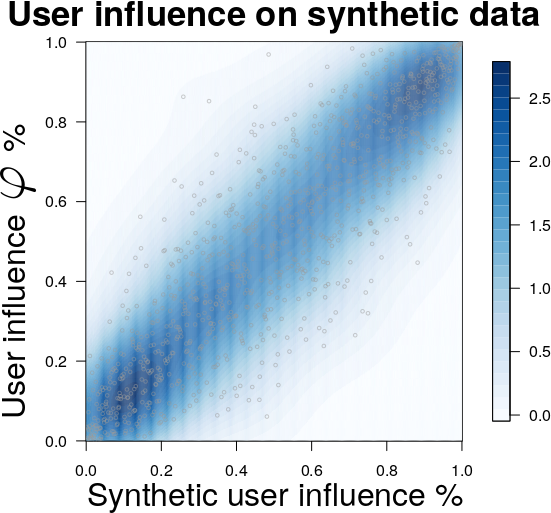
\includegraphics[height=\myheight\textheight]{synthetic-user-influence}
		\label{subfig:artificial-compare}
	}
	\subfloat[] {
		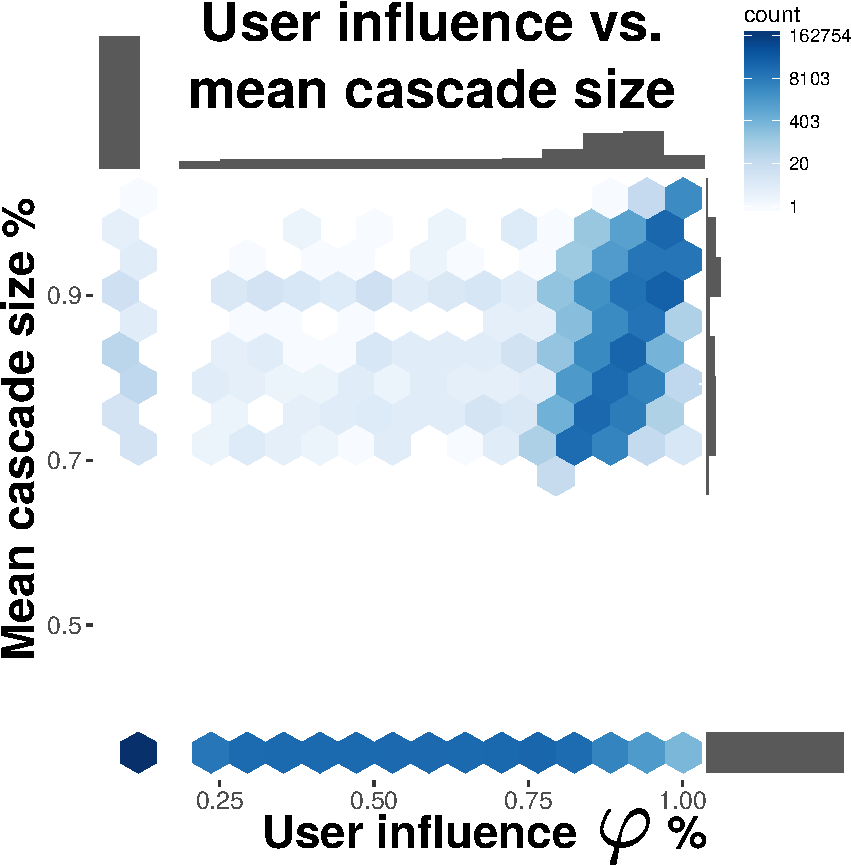
\includegraphics[height=\myheight\textheight]{influence-vs-mcsize}
		\label{subfig:mean-cascade-size}
	}\\
	\subfloat[] {
		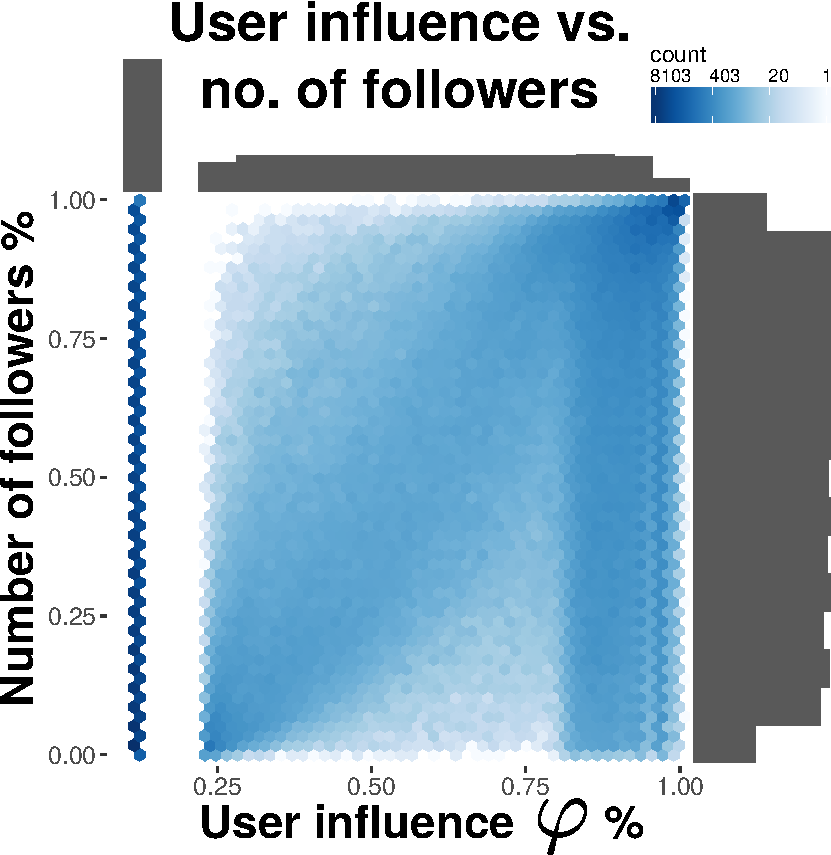
\includegraphics[height=0.19\textheight]{influence-vs-followersCount}
		\label{subfig:no-followers}
	}
%	\subfloat[] {
%		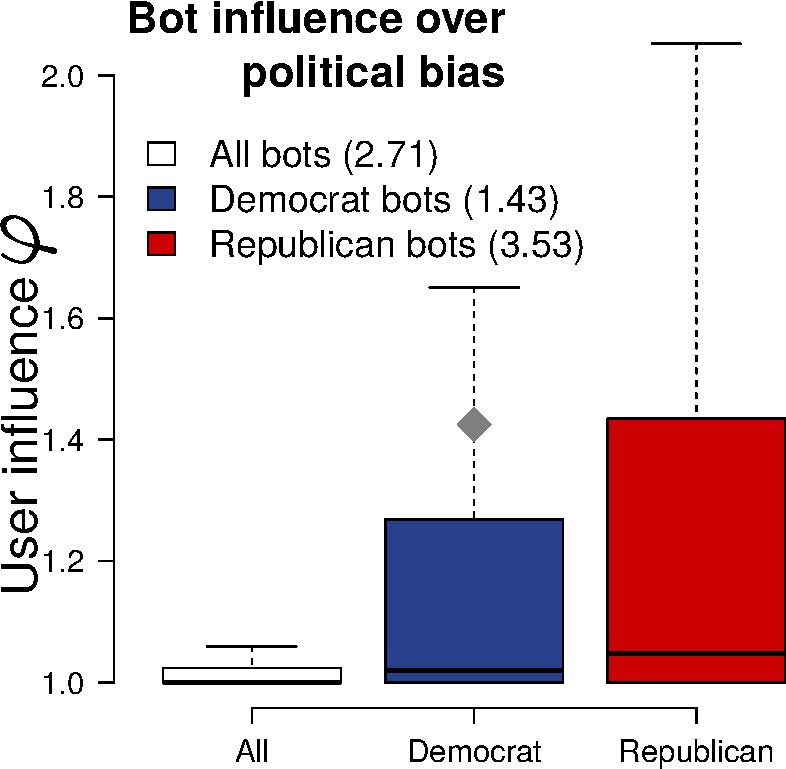
\includegraphics[height=\myheight\textheight]{BOTS_boxplot-influence-vs-political-bias}
%	}
	\caption{ 
		Evaluation of the user influence measure.
		\textbf{(a)} 2D density plot (shades of blue) and scatter-plot (gray circles) of user influence against the ground truth on a synthetic dataset.
		\textbf{(b)(c)} Hexbin plot of user influence percentile (x-axis) against mean cascade size percentile (b) and the number of followers (c) (y-axis) on \debate.
		The color intensity indicates the number of users in each hex bin.
		1D histograms of each axis are shown using gray bars.
		Note $72.3\%$ of all users that initiate cascades are never retweeted.
	}
%	\label{fig:holdout-ll}
%	\captionmoveup
\end{figure}

%!TEX root = main.tex

\begin{figure*}[htbp]
	\centering
	\newcommand\myheight{0.131}
	\subfloat[] {
		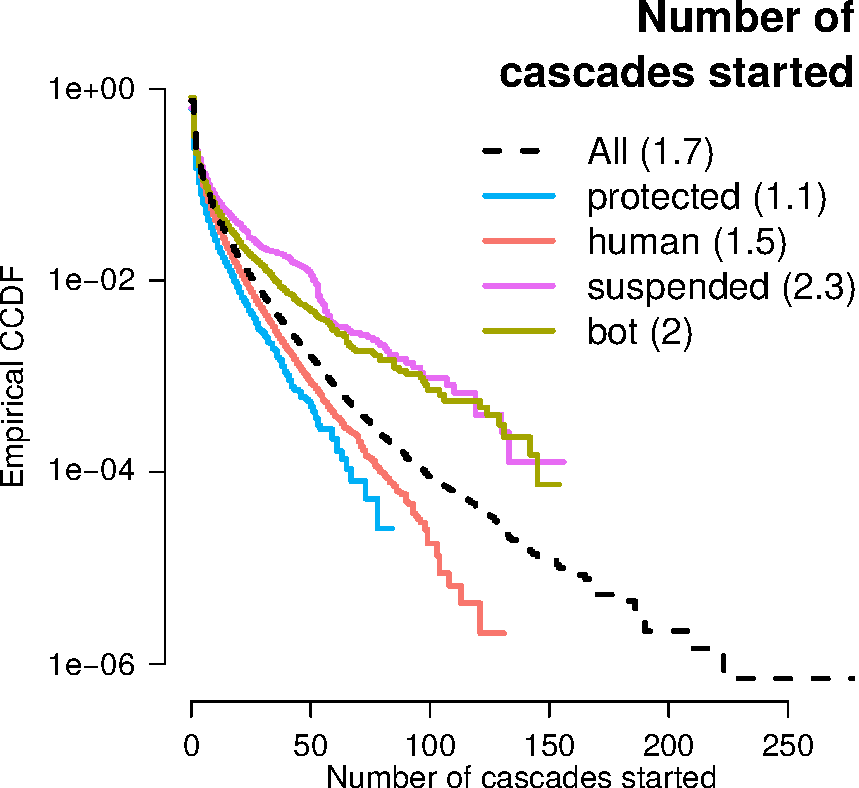
\includegraphics[height=\myheight\textheight]{bot-a-number-of-diffusions}
		\label{subfig:no-cascades}
	}
	\subfloat[] {
		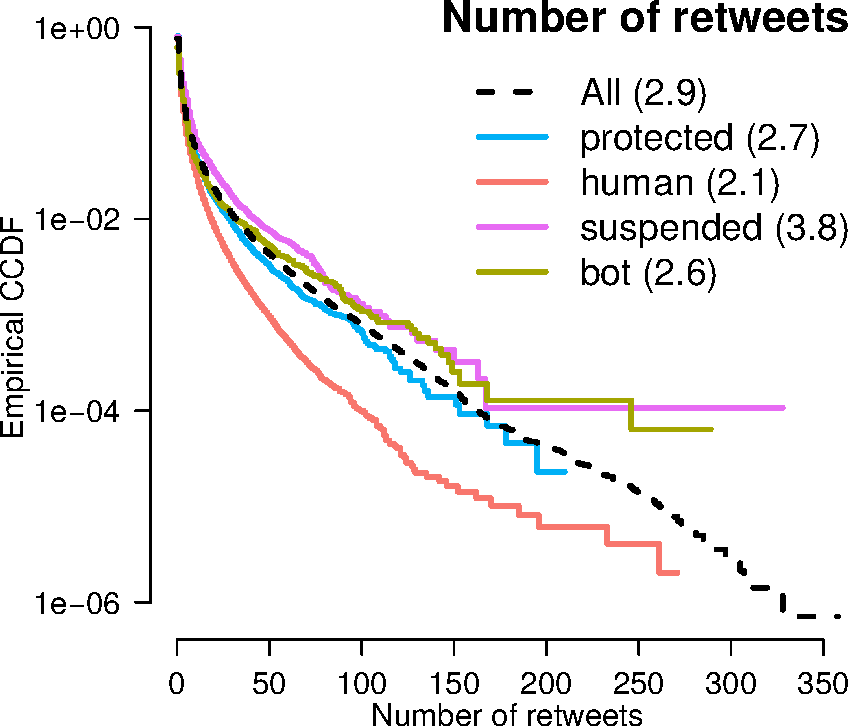
\includegraphics[height=\myheight\textheight]{bot-b-number-of-retweets}
		\label{subfig:no-retweets}
	}
	\subfloat[] {
		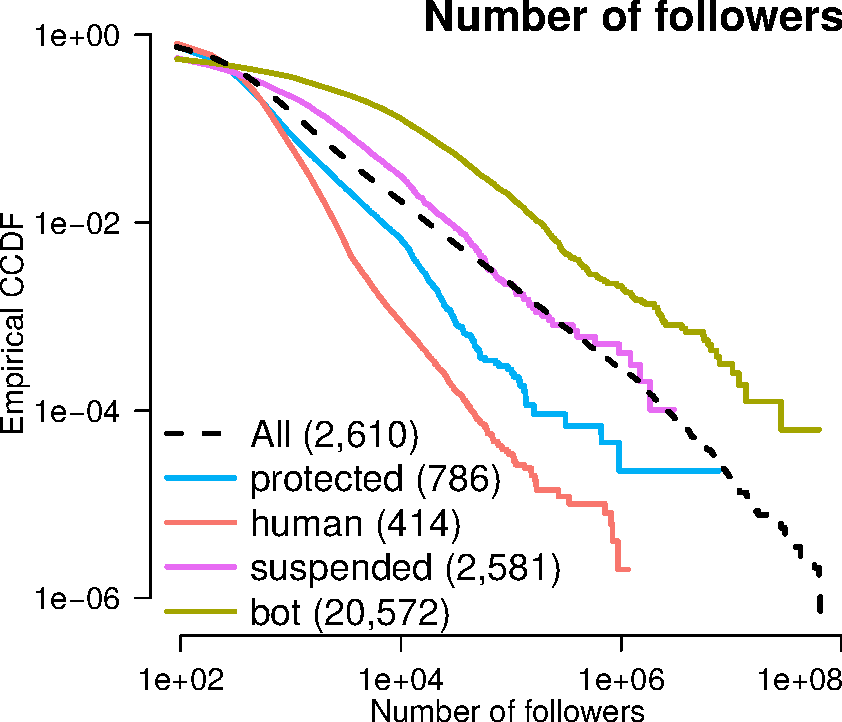
\includegraphics[height=\myheight\textheight]{bot-c-followers-count-CCDF}
		\label{subfig:numfolowers-CCDF}
	}
	\subfloat[] {
		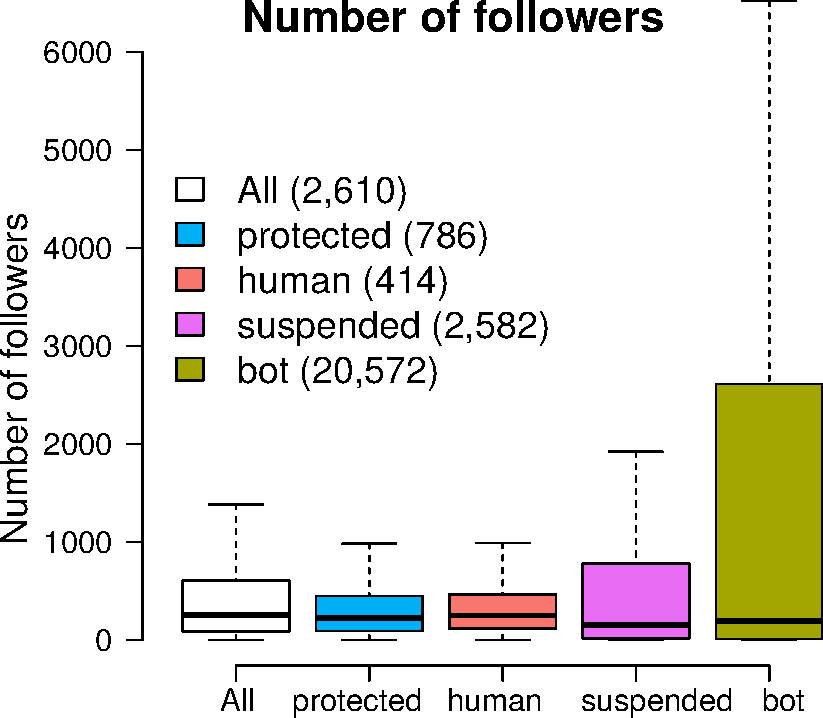
\includegraphics[height=\myheight\textheight]{bot-d-followers-count-boxplot}
		\label{subfig:numfolowers-boxplot}
	}
	\subfloat[] {
		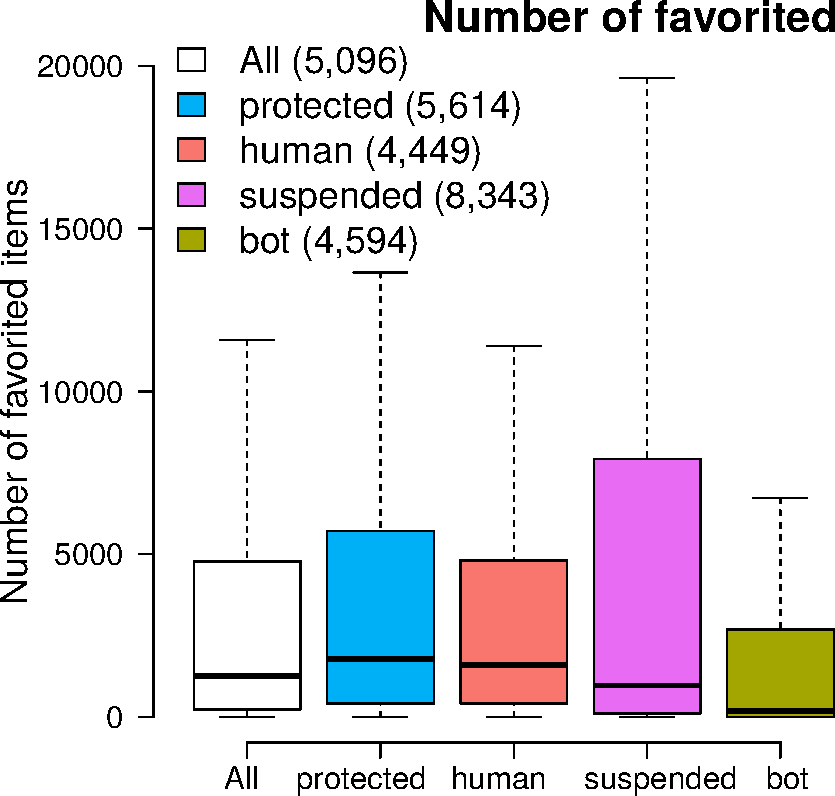
\includegraphics[height=\myheight\textheight]{bot-e-favorites-count}
		\label{subfig:numfavorited}
	}
	\caption{ 
		Profiling behavior of the \Protected, \Human, \Suspended and \Bot populations in the \debate dataset.
		The numbers in parentheses in the legend are mean values.
		\textbf{(a)} CCDF of the number of Twitter diffusion cascades started.
		\textbf{(b)} CCDF of the number of retweets. 
		\textbf{(c)(d)} CCDF (c) and boxplots (d) of the number of followers. 
		\textbf{(e)} Number of items favorited.
	}
	\label{fig:bot-profiling}
%	\captionmoveup
\end{figure*}

%\verify{RJA comment: I was initially wondering if it is necessary to have "$\varphi(u)$ \%" in the figures, thinking it could just be stated in 4.3 that it is normalised (percentiles) and then can just use $\varphi(u)$ throughout. But then I realised that e.g. in Figure 7 the means of unnormalised influence are presented. So I've slightly modified text in 4.3 to highlight we use both.}

In this section, we evaluate our proposed algorithm and measure of user influence.
In Sec~\ref{subsec:ground-truth}, we evaluate on synthetic data against a known ground truth.
In Sec.~\ref{subsec:two-alternatives}, we compare the $\varphi(u)$ measure (defined in Sec.~\ref{subsec:user-influence-measure}) against two alternatives: the number of followers and the mean size of initiated cascades.

\subsection{Evaluation of user influence}
\label{subsec:ground-truth}

%\textbf{Influence is unobserved in real data.}
Evaluating user influence on real data presents two major hurdles.
The first is the lack of ground truth, as user influence is not directly observed.
%While it is possible to manually assess influence, this approach does not scale to the 1.5M users in our dataset.
The second hurdle is that the diffusion graph is unknown, which renders impossible comparing to state-of-the-art methods which require this information (e.g. ConTinEst~\cite{Du2013}).
%Current state of the art methods for uncovering the diffusion structure (e.g. NetInf~\cite{gomez2010inferring}) do not scale to the number of users in our dataset.
%This is because these methods assume a large number of cascades occurring in a rather small social neighborhood.
%
%\verify{RJA comment: The above paragraph is very interesting and I wonder if some of it could be moved into Section 2.1 since there are general points about what is influence, how to measure it etc, and it covers some of the points made in 2.1, but in a different way.  But regardless of position of the material, I have some clarifying questions.  I'm trying to pose the questions that someone who knows about social influence but not these techniques directly may ask. To make this as efficient as possible I'm going to attempt to re-write the above paragraph so you see how I understand it and where misunderstanding may be arising.
%
%Evaluating user influence on real data presents three major hurdles.
%The first is the lack of ground truth, as user influence is not directly observed: in general it is not feasible nor even meaningful to ask people "who are you influenced by?" or "who do you influence?" and this infeasibility is compounded in the context of thousands of users participating in debate related activity on Twitter.
%Given that user influence is not directly observable, interest (especially in the context of social media) has turned to estimating or inferring influence based on a user's contribution to the diffusion of information.
%However in general there will be many diffusion trees that need to be taken account of and so the second hurdle is the need to infer the underlying or latent social network that generated the diffusion trees, and influence is then computed over that social network. This is the approach used by state-of-the-art methods such as ConTinEst~\cite{Du2013}. In the case of user influence on Twitter, we are presented with a third hurdle: we do not have the complete retweet cascade data.
%Current state of the art methods for uncovering the diffusion structure (NetInf and its extension~\cite{gomez2010inferring,gomez2013structure}) do not scale to the number of users in our dataset.
%This is because these methods assume a large number of cascades occurring in a rather small social neighborhood.
%}
%
%\verify{RJA comment: There are in fact two types of latent structure that we are dealing with our particular example. First we do not have the complete diffusion tree data and so we need to deal with this by evaluating all of the possible diffusion scenarios. Second, even if we had complete diffusion tree data we still do not know the latent \emph{social network} which has generated the diffusion trees.}
%In this section, we reproduce ConTinEst's evaluation against a known ground truth on a synthetic dataset.
In this section, evaluate our algorithm against a known ground truth on a synthetic dataset, using the same evaluation approach used for ConTinEst.

\textbf{Evaluation on synthetic data.}
%We compare against ConTinEst~\cite{Du2013} on a synthetic dataset.
We evaluate on synthetic data using the 
%We follow the synthetic data evaluation 
protocol previously employed in~\cite{Du2013}.
We use the simulator in \cite{Du2013} to generate an artificial social network with 1000 users.
We then simulate 1000 cascades through this social network, starting from the same initial user.
The generation of the synthetic social network and of the cascades is detailed in the online supplement~\cite[annex~C]{supplemental}.
%\ref{si-sec:generation-artificial}
Similar to the retweet cascades in \debate, each event in the synthetic cascades has a timestamp and an associated user.
Unlike the real retweet cascades, we know the real diffusion structure behind each synthetic cascade.
%We compute the synthetic user influence as performed in ConTinEst~\cite{Du2013}.
For each user $u$, we count the number of nodes reachable from $u$ in the diffusion tree of each cascade.
We compute the influence of $u$ as the mean influence over all cascades.
ConTinEst~\cite{Du2013} has been shown to asymptotically approximate this synthetic user influence.

%\textbf{Results.}
We use our algorithm introduced in Sec.~\ref{subsec:user-influence-mt} on the synthetic data, to compute the measure $\varphi(u)$ defined in Eq.~\ref{eq:user-infl-casin}.
%We set the parameter of the temporal decay at $r = 6.8 \times 10^{-4}$, determined using linear search on a sample of 20 real retweet diffusions (details in the online supplement~\cite[annex~D]{supplemental}).
We plot in Fig.~\ref{subfig:artificial-compare} the 2D scatter-plot and the density plot of the synthetic users, with our influence measure $\varphi$ on the y-axis and the ground truth on the x-axis (both in percentiles).
Visibly, there is a high agreement between the two measures, particularly for the most influential and the least influential users.
The Spearman correlation coefficient of the raw values is $0.88$.
This shows that our method can output reliable user influence estimates in the absence of any information about the structure of the diffusions.

\subsection{Comparison with other influence metrics}
\label{subsec:two-alternatives}

We compare the influence measure $\varphi(u)$ against two alternatives that can be computed on \debate.

%\textbf{Mean size of initiated cascades} (of a user $u$) is the average number of users reached by content emitted by $u$ and it represents by definition the user influence~\cite{Du2013}.
%\verify{RJA comment: I don't agree with the above statement (note: haven't read Du et al....). I think it represents *one* definition of user influence but not *the* definition of user influence (if it did, then we'd be using it rather than the complicated approach we use here). I think "content emitted by u" is confusing because in fact we are talking about original tweets here, not retweets. How about we say something like: 

\textbf{Mean size of initiated cascades} (of a user $u$) is the average number of users reached by original content authored by $u$.
% and it is one definition user influence~\cite{Du2013}. 
It should be noted that this measure does not capture $u$'s role in diffusing content authored by someone else.
%}
In the context of Twitter, mean size of initiated cascades is the average number of users who retweeted an original tweet authored by $u$: we compute this for every user in the \debate dataset, and we plot it against $\varphi(u)$ in Fig.~\ref{subfig:mean-cascade-size}.
Few users have a meaningful value for mean cascade size: 
$55\%$ of users never start a cascades (and they are not accounted for in Fig.~\ref{subfig:mean-cascade-size}); 
out of the ones that start cascades $72.3\%$ are never retweeted and they are all positioned at the lowest percentile (shown by the 1D histograms in the plot).
%(they all have an equal mean cascade rank of $36.1\%$ on the y-axis of the figure).
%\TODO{RJA}{I think "meaningful value" needs to be clarified. If I authored a single original tweet but no-one retweeted me, then the mean cascade size would be 0 and that is meaningful, I think? However if I never authored an original tweet then I can see that mean cascade size is not computable for me.  Relatedly, the text above implies that $45\%$ of users start a cascade (i.e. author an original tweet) but that doesn't correspond to "very few" and also it doesn't really match up with the histogram on vertical axis.  Or now I'm thinking that you've lumped the users who never started a cascade with those who did start a cascade but it has size 0 because no-one retweeted. I don't understand what is meant by mean cascade rank. }
%
It is apparent that the mean cascade size metric detects the influential users that start cascades, and it correlates with $\varphi(u)$.
However, it misses highly influential users who never initiate cascades, but who participate by retweeting. Examples are user \textit{@SethMacFarlane} (the actor and filmmaker Seth MacFarlane, 10.8 million followers) or user \textit{@michaelianblack} (comedian Michael Ian Black, 2.1 million followers), both with $\varphi$ in the top $0.01\%$ most influential users.

\textbf{Number of followers} is one of the simplest measures of direct influence used in literature~\cite{Mishra2016,Zhao2015}.
While being loosely correlated with $\varphi(u)$ (visible in Fig.~\ref{subfig:no-followers}, Pearson $r = 0.42$), it has the drawback of not accounting for any of the user actions, such as an active participation in discussions or generating large retweet cascades.
For example, user \textit{@PoliticJames} (alt-right and pro-Trump, 2 followers) emitted one tweet in \debate, which was retweeted 18 times and placing him in the top $1\%$ most influential users.
Similarly, user \textit{@tiwtter1tr4\_tv} (now suspended, 0 followers) initiated a cascade of size 58 (top $1\%$ most influential).
Interestingly, half of the accounts scoring on the bottom $1\%$ by number of followers and top $1\%$ by influence are now suspended or have very high botness scores.

%\verify{RJA comment: The evaluation section is really useful for illustrating how our measure of influence can capture what number of followers and number of retweets (received) doesn't. This is just a comment, not for inclusion...}

%!TEX root = main.tex

\section{Results and findings}
\label{sec:results-findings}

In this section, we present an analysis of the interplay between botness, political behavior (polarization and engagement) and influence.
In Sec.~\ref{subsec:polarization-botness}, we first profile the activity of users in the four reference populations; next, we analyze the political polarization and engagement, and their relation with the botness measure.
Finally, in Sec.~\ref{subsec:user-influence-results} we tabulate user influence against polarization and botness, and we construct \emph{the polarization map}.

%!TEX root = main.tex

\begin{figure}[!tb]
	\centering
	{
	\newcommand\myheight{0.145}
	\subfloat[] {
		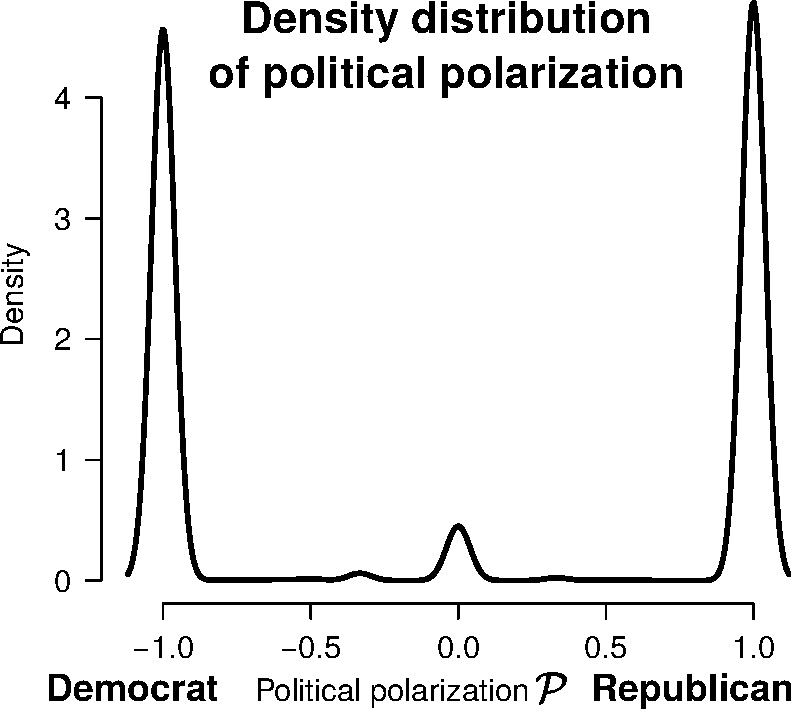
\includegraphics[height=\myheight\textheight]{a-density-distribution-political-bias}
		\label{subfig:distribution-political-bias}
	}
	\subfloat[] {
		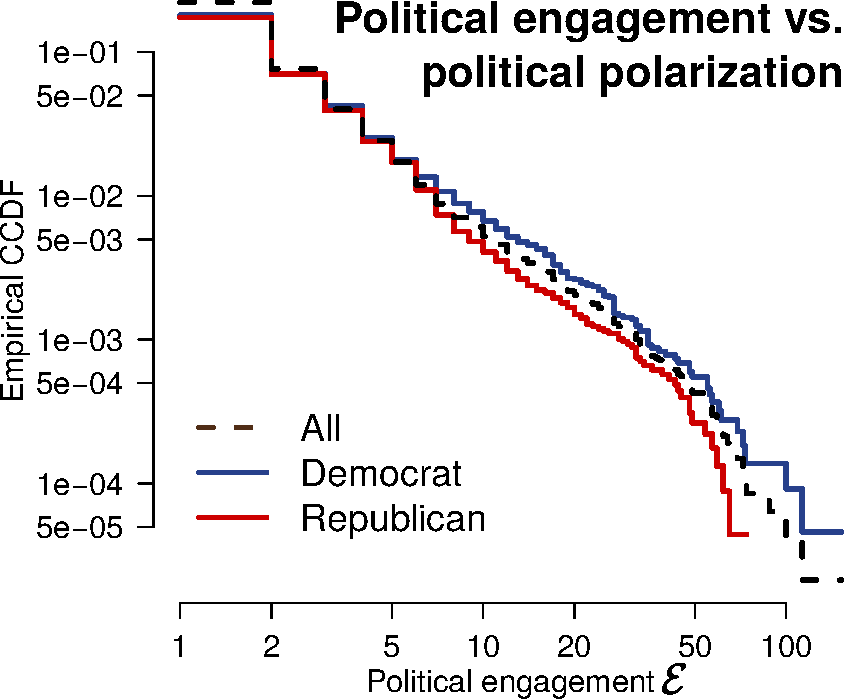
\includegraphics[height=\myheight\textheight]{b-CCDF-bias_engagement-vs-political-bias}
		\label{subfig:engagement-vs-political}
	}}
	\\
	{
	\newcommand\myheight{0.16}
	\subfloat[] {
		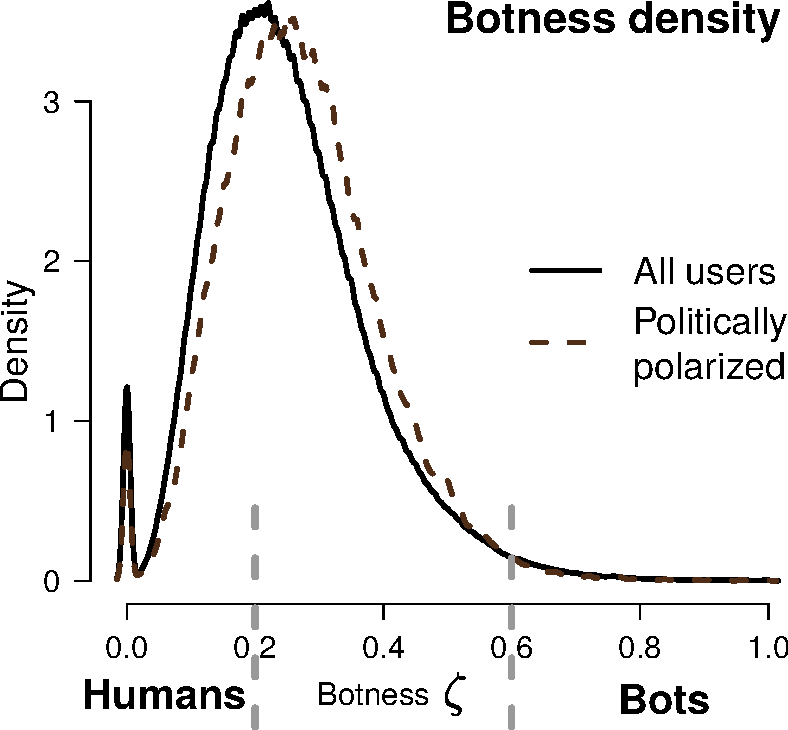
\includegraphics[height=\myheight\textheight]{botscore-density-all-polarization}
		\label{subfig:botscore-density}
	}
	\subfloat[] {
		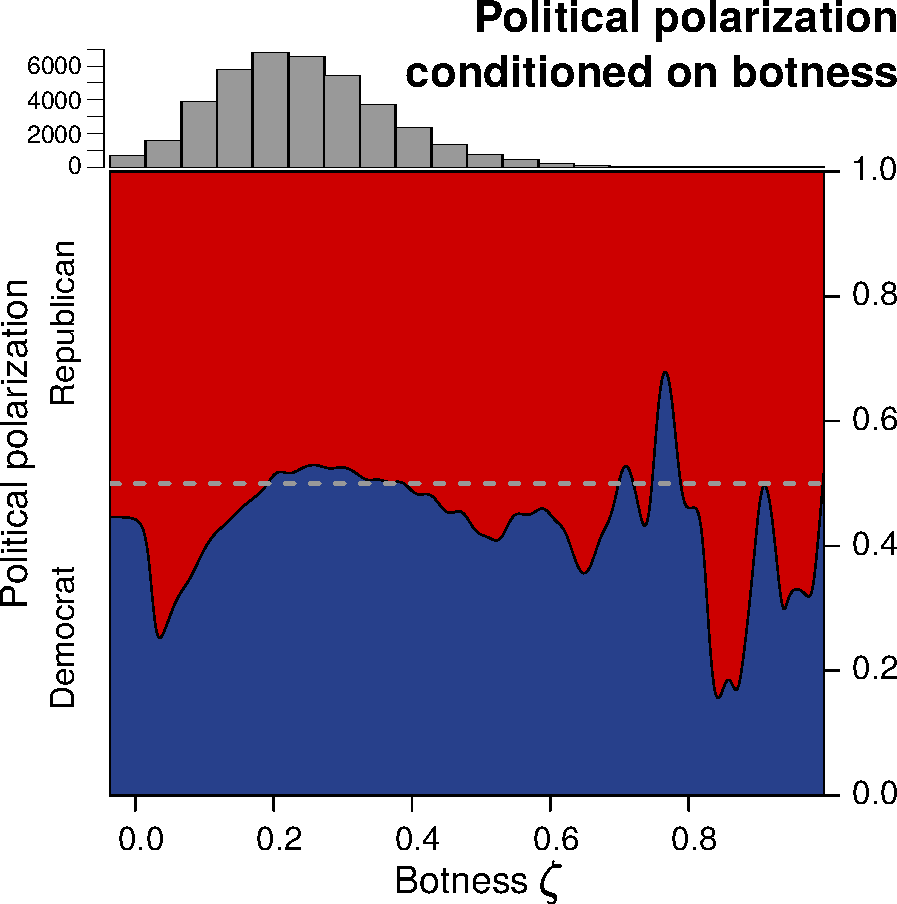
\includegraphics[height=\myheight\textheight]{botscore-conditional-density}
		\label{subfig:botscore-conditional-density}
	}}
	\\
	{ 
	\newcommand\myheight{0.145}
	\subfloat[] {
		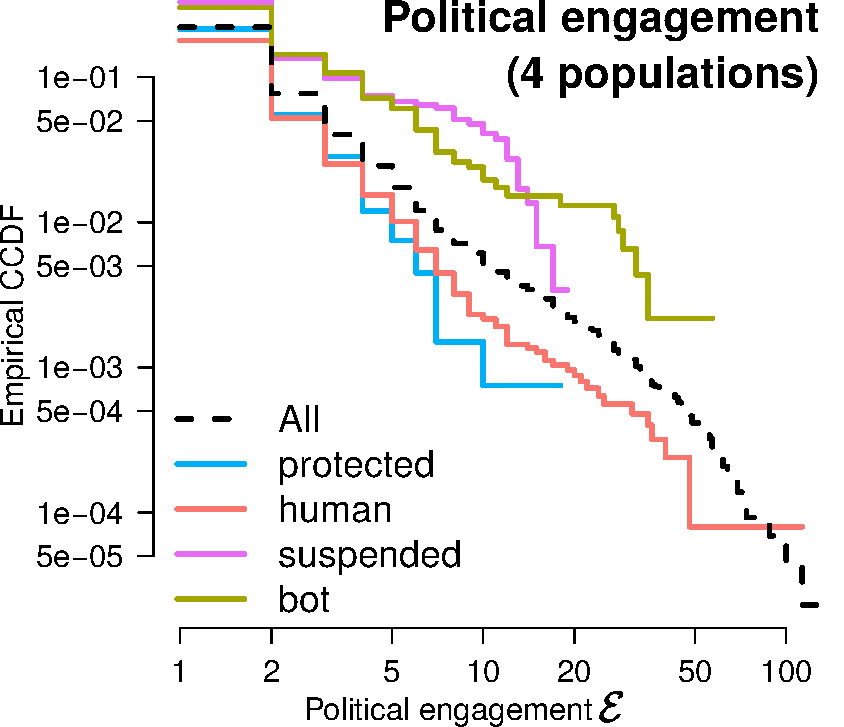
\includegraphics[height=\myheight\textheight]{c-pol-engagement-vs-botscore}
		\label{subfig:engagement-vs-botscore}
	}
	\subfloat[] {
		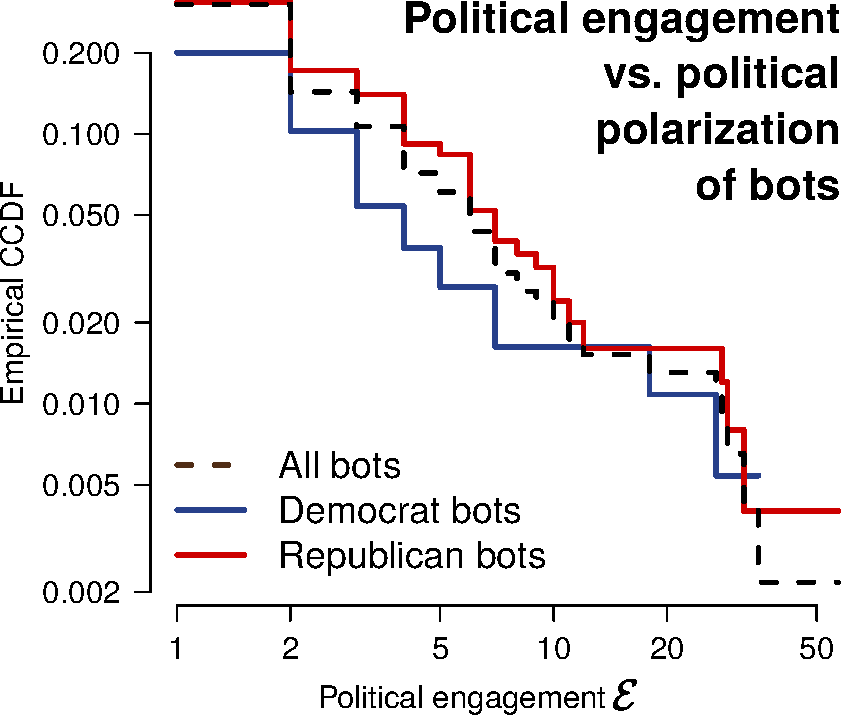
\includegraphics[height=\myheight\textheight]{d-BOTS_pol-engagement-vs-botscore}
		\label{subfig:BOTS_pol-engagement-vs-botscore}
	}
	}
	\caption{ 
		Political polarization, engagement and botness.
		\textbf{(a)} The density distribution of political polarization $\mathcal{P}$. %shows two peaks at -1 and 1, corresponding to strongly democrat and strongly republican respectively.
		\textbf{(b)} Log-log plot of the CCDF of political engagement $\mathcal{E}$ 
%		overall (dashed line), and 
		for the Democrat and Republican populations.
		% (blue and red lines respectively).
		%complementary cumulative distribution function shows that the political engagement score is long-tail distributed, with democrats being slightly more engaged than republicans overall.
		\textbf{(c)} The density distribution of botness $\zeta$ for the entire population (solid line) and the politically polarized population (dashed line). 
		%shows a large peak around $[0.1, 0.4]$ and a long tail.
		%Politically polarized users have slightly higher bot scores.
%		The dashed gray vertical lines show the threshholds for constructing the references human population ($\zeta \in [0, 0.2]$) and bot population ($\zeta \in [0.6, 1]$).
		\textbf{(d)} The conditional density of polarization conditioned on botness.
		The top panel shows the volumes of politically polarized users in 30 bins.
		\textbf{(e)(f)} CCDF of political engagement for the reference populations (e) and for the polarized \Bot populations (f).
		%\TODO{MAR}{Message in text: the \mbox{\Bot} and \mbox{\Suspended} populations are more politically engaged than the \mbox{\Human} and \mbox{\Protected}.}
	}
	\label{fig:bot-polarization}
%	\captionmoveup
\end{figure}

\subsection{Political behavior of humans and bots}
\label{subsec:polarization-botness}

\textbf{Twitter activity across four populations.}
We measure the behavior of users in the four reference populations defined in Sec.~\ref{subsec:political-polarization-measures} using several measures computed from the Twiter API.
The number of cascades started (i.e., number of original tweets) and the number of posted retweets are simple measures of activity on Twitter, and they are known to be long-tail distributed~\cite{Cha2010}.
%\TODO{RJA}{Am I correct that number of cascades initiated is the same thing as the number of original tweets authored during the 2 hours, since we saw previously that a cascade can have length of zero? Also I'm clarifying in previous sentence that "number of retweets" is the retweets sent/made, not received?. Finally, not a big deal but do we really expect that number of cascades initiated in 2 hour period would be power law distributed?  I expect it would be unequally distributed, but not long-tail.  Not big deal...}
Fig.~\ref{subfig:no-cascades} and~\ref{subfig:no-retweets} respectively plot the log-log plot of the empirical Complementary Cumulative Distribution Function (CCDF) for each of the two measures.
It is apparent that users in the \Bot and \Suspended populations exhibit higher levels of activity than the general population, whereas the \Human and \Protected populations exhibit lower level.
Fig.~\ref{subfig:numfolowers-CCDF} and~\ref{subfig:numfolowers-boxplot} plot the number of followers and present a more nuanced story:
the average bot user has 10 times more followers than the average human user;
however, bots have a median of $190$ followers, less than the median $253$ followers of human users.
In other words, some bots are very highly followed, but most are simply ignored.
Finally, Fig.~\ref{subfig:numfavorited} shows that bots favorite less than humans, indicating that their activity patterns differ from those of humans.
%\TODO{RJA}{I would get rid of Figure 6e since not really important to the story, and we are struggling to get it under 10 pages, not that it will save much.}
%
%the bot score against user political polarization (see Sec.~\ref{subsec:political-polarization-measures} and~\ref{subsec:political-polarization-results}) --, and against a number of measures provided by the Twitter API -- the number of followers, the number of friends, the number of favorited, the number of cascades initiated and the number of retweets. 
%
%\TODO{MAR}{Warning: outdated story. Check \mbox{Fig.~\ref{fig:bot-profiling}} for updated story.}
%\verify{
%Story here goes like this:
%\begin{itemize}
%	\item bots tend to be more active on Twitter, they start more cascades and they retweet more (Fig~\ref{subfig:tweets-vs-botscore} and~\ref{subfig:retweets-vs-botscore} respectively); 
%	mean number of cascades per bot is 2, and 2.3 for the suspended versus 1.1 for humans and 1.1 for protected;
%	the distribution of number of started cascades and retweets has a longer tail for bots than the general population and for humans.
%
%%	\item it is known that the distribution of number of followers and friends (users followed by a given users) is long tail.
%	However, the distributions for the bot and suspended populations are even more skewed: the median number of followers for a bot is $190$ (less than the average user of ), but the mean is $20,572$ (ten times more than the average user).
%	This indicates that most bots are not followed, while few get considerable following;
%	
%%	\item bots tend to favorite less than the average users (Fig.~\ref{subfig:numfavorited-vs-botscore}).
%\end{itemize}
% }
%
%This section profiles three of the measures proposed in Sec.~\ref{sec:four-measures}: the botness, the political polarization and the political engagement.
%the bot score against user political polarization (see Sec.~\ref{subsec:political-polarization-measures} and~\ref{subsec:political-polarization-results}) --, and against a number of measures provided by the Twitter API -- the number of followers, the number of friends, the number of favorited, the number of cascades initiated and the number of retweets. 
%A number of finding emerge from the analysis in presented in Fig.~\ref{fig:bot-polarization}, particularly about the polarization and engagements of bot-like accounts.

%\verify{RJA comment: Some fairly minor comments on Figure 5...In 5a there should be $\mathcal{P}$ after "Political polarization" on the x-axis. I think a better title for 5f is "Political engagement vs political polarization of bots" or similar.}

%\verify{RJA comment: Minor comment on Figure 7 - I don't think the labeling of the color scale is correct? If the colour shows the ratio of the densities of pop of D and R, shouldn't it range from 0 to infinity or something, but not +1 to -1.}

\textbf{Political polarization and engagement.}
The density distribution of political polarization (Fig.~\ref{subfig:distribution-political-bias}) shows two peaks at -1 and 1, corresponding to strongly pro-Democrat and strongly pro-Republican respectively. 
The shape of the density plot is consistent with the sizes of Republican and Democrat populations (Sec.~\ref{subsec:political-polarization-measures}), and the extreme bi-modality can be explained by the clear partisan nature of the chosen hashtags and by the known political polarization of users on Twitter \cite{conover.2011,barbera.2015}, which will be greatly enhanced in the context of a political debate.
%This validates our political polarization coding schema (defined in Sec.~\ref{subsec:political-polarization-measures} 
%\TODO{MAR}{why and how does it validate it? is there previous work that states that Twittersphere is polarized?} 
%and shows that most users are clearly biased towards one party or the other (with a small set of users who `hashtag-dump' in a somewhat random fashion). 
Fig.~\ref{subfig:engagement-vs-political} presents the log-log plot of the CCDF of the political engagement, which shows that the political engagement score is long-tail distributed, with \emph{pro-Democrats slightly more engaged than pro-Republicans overall} (t-test significant, p-val $ = 0.0012$).

%following has been addressed
%\verify{RJA comment: I will be adding material to "related work" section that shows there is significant political polarization on Twitter but other authors have not found the extent of polarization displayed in Figure 4(a). I'm wondering how polarization was measured here. It looks like it might have been that you are classified as D if you used more D hashtags and vice-versa for R? The hashtag dumpers were 50:50 in their use? I think a political scientist looking at 4(a) might be dubious and think while bi-modal distribution is reasonable (given it was politically event) there would have been more users in the middle i.e. not clearly R nor D?}
%\TODO{@RJA}{Do the changes in the above paragraph address your concerns? Needs a reference there.}

\textbf{Botness and political polarization.}
The distribution of botness $\zeta$ exhibits a large peak around $[0.1, 0.4]$ and a long tail (Fig.~\ref{subfig:botscore-density}). 
The dashed gray vertical lines show the threshholds used in Sec.~\ref{subsec:bot-detection} for constructing the reference \Human ($\zeta \in [0, 0.2]$) and \Bot ($\zeta \in [0.6, 1]$) populations.
%The density distribution for politically polarized users is skewed towards higher botness, showing that politically polarized users are more likely to be automated systems.
Fig.~\ref{subfig:botscore-conditional-density} shows the conditional density of polarization conditioned on botness.
For both high botness scores (i.e., bots) and low botness scores (humans) the likelihood of being pro-Republican is consistently higher than that of being pro-Democrat, while users with mid-range botness are more likely to be pro-Democrat.
%While the likelihood of being pro-Democrat or pro-Republican varies significantly with botness, for high botness scores 
In other words, \emph{socialbots accounts are more likely to be pro-Republican than to be pro-Democrat}.

\textbf{Political engagement of bots.}
Fig.~\ref{subfig:engagement-vs-botscore} shows the CCDF of political engagement of the four reference populations, and it is apparent that the \Bot and \Suspended populations exhibit consistently higher political engagement than the \Human and \Protected populations. 
Fig.~\ref{subfig:BOTS_pol-engagement-vs-botscore} shows the CCDF of political engagement by the political partisanship of bots and we find that pro-Republican \Bot accounts are more politically engaged than their pro-Democrat counterparts.
In summary, \emph{socialbots are more engaged than humans (p-val = $8.55 \times 10^{-5}$), and pro-Republican bots are more engaged than their pro-Democrat counterparts (p-val = 0.1228)}.

%!TEX root = main.tex

\begin{figure*}[htbp]
	\centering
	\newcommand\myheight{0.162}
	\subfloat[] {
		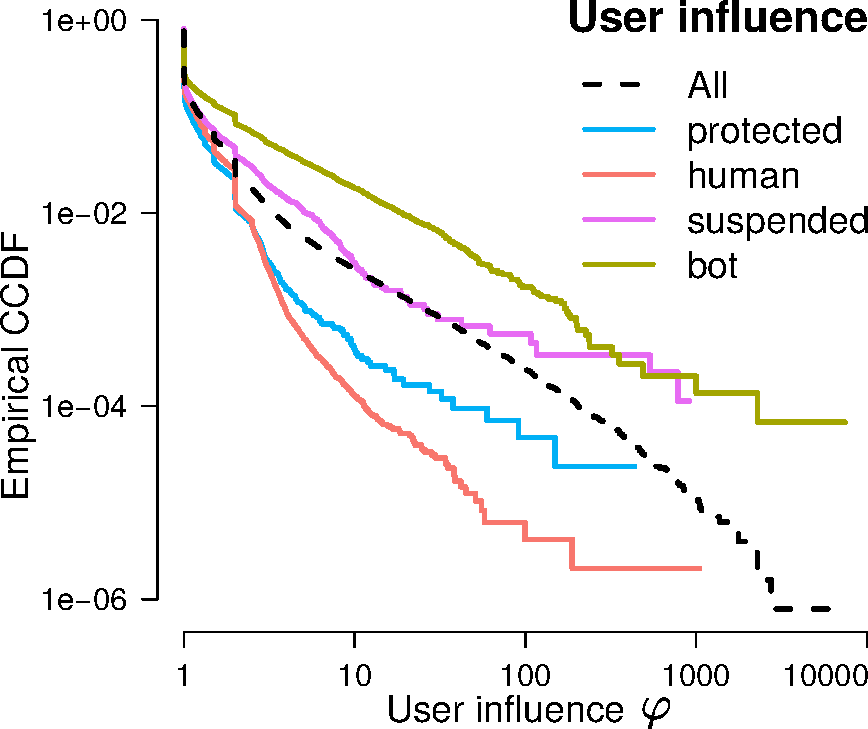
\includegraphics[height=\myheight\textheight]{2017-11-13-CCDF-influence-4-populations}
		\label{subfig:user-infl-CCDF}
	}
	\subfloat[] {
		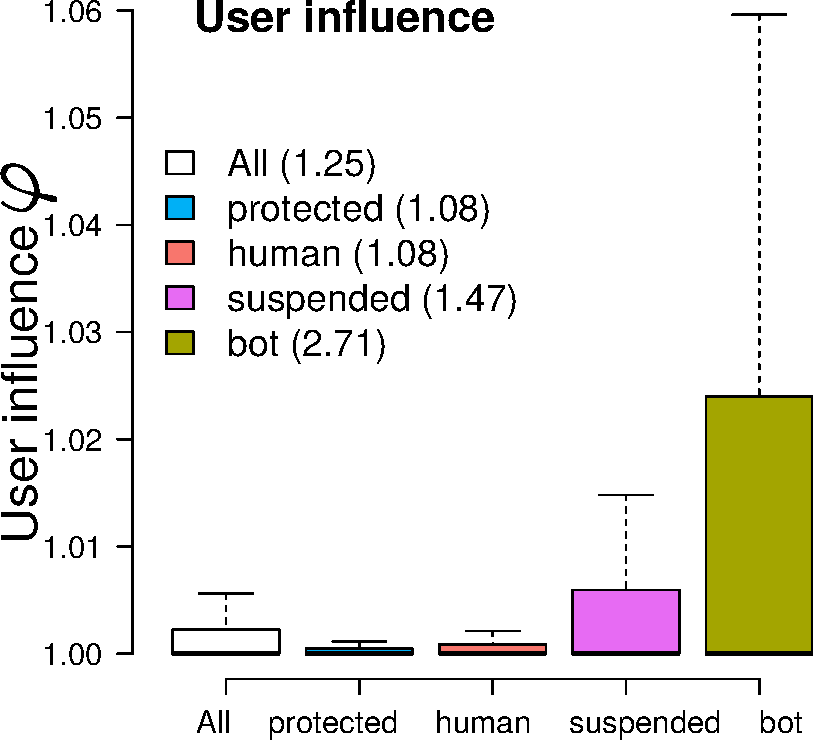
\includegraphics[height=\myheight\textheight]{2017-11-13-boxplot-influence-4-populations}
		\label{subfig:user-infl-boxplots}
	}
	\subfloat[] {
		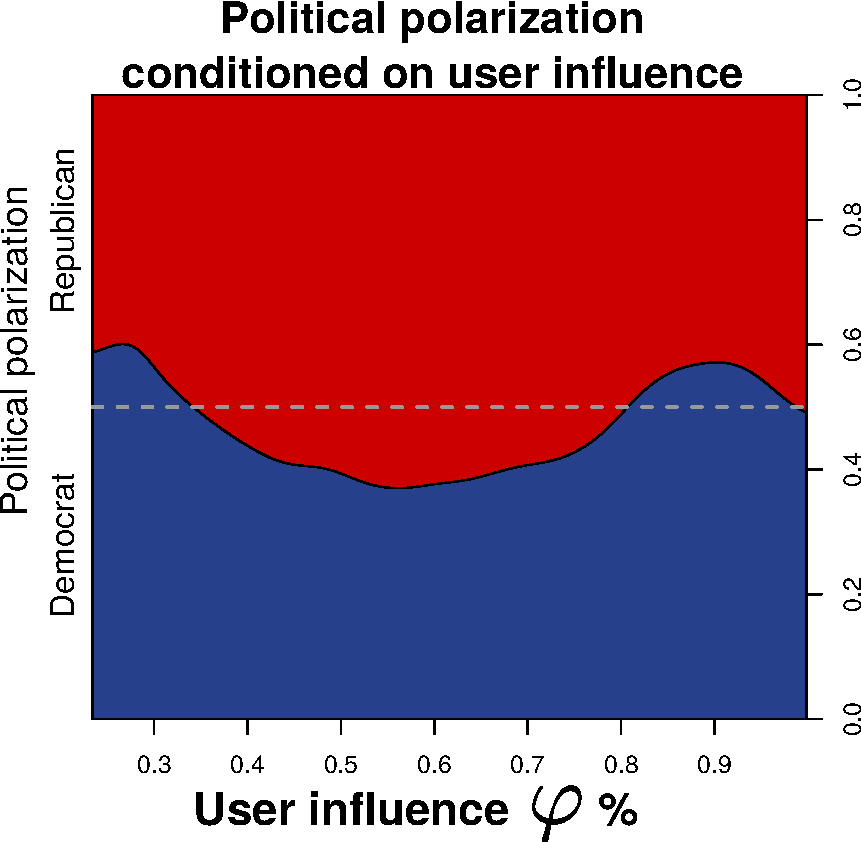
\includegraphics[height=\myheight\textheight]{influence_conditional_density}
		\label{subfig:polarization-conditioned-user-infl}
	}
	\subfloat[] {
		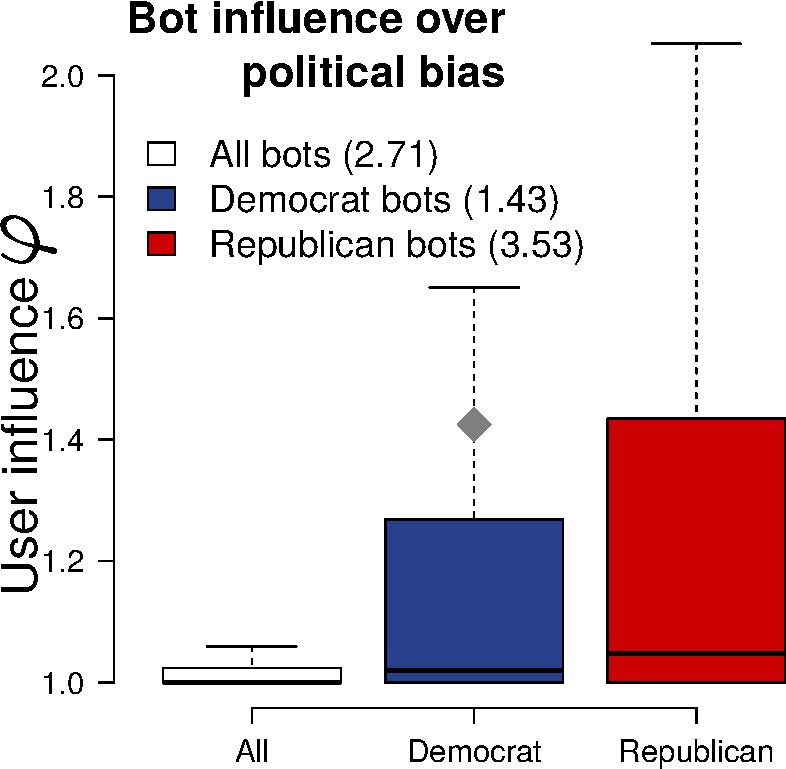
\includegraphics[height=\myheight\textheight]{BOTS_boxplot-influence-vs-political-bias}
		\label{subfig:bot-influence}
	}
	\caption{ 
		Profiling influence, and linking to botness and political behavior.
		\textbf{(a)(b)} User influence $\varphi(u)$ for the reference populations, shown as log-log CCDF plot (a) and boxplots (b).
%		The influence in each of the four reference populations is long-tail distributed.
%		\textbf{(b)} Boxplot of user influence for the four bot populations -- 
		\textbf{(c)} Probability distribution of polarization, conditional on $\varphi(u) \%$.
		\textbf{(d)} Boxplots of user influence for the pro-Democrat and pro-Republican \Bot users.
		% (dashed line), and for the democrat and republican polarized populations (blue and red lines respectively).
		%\TODO{MAR}{Message in text: republican bots are more engaged than democrat bots.}
		Numbers in parenthesis show mean values.
	}
%	\label{fig:holdout-ll}
%	\captionmoveup
\end{figure*}

%!TEX root = main.tex

\begin{figure}[tb]
	\centering
	
	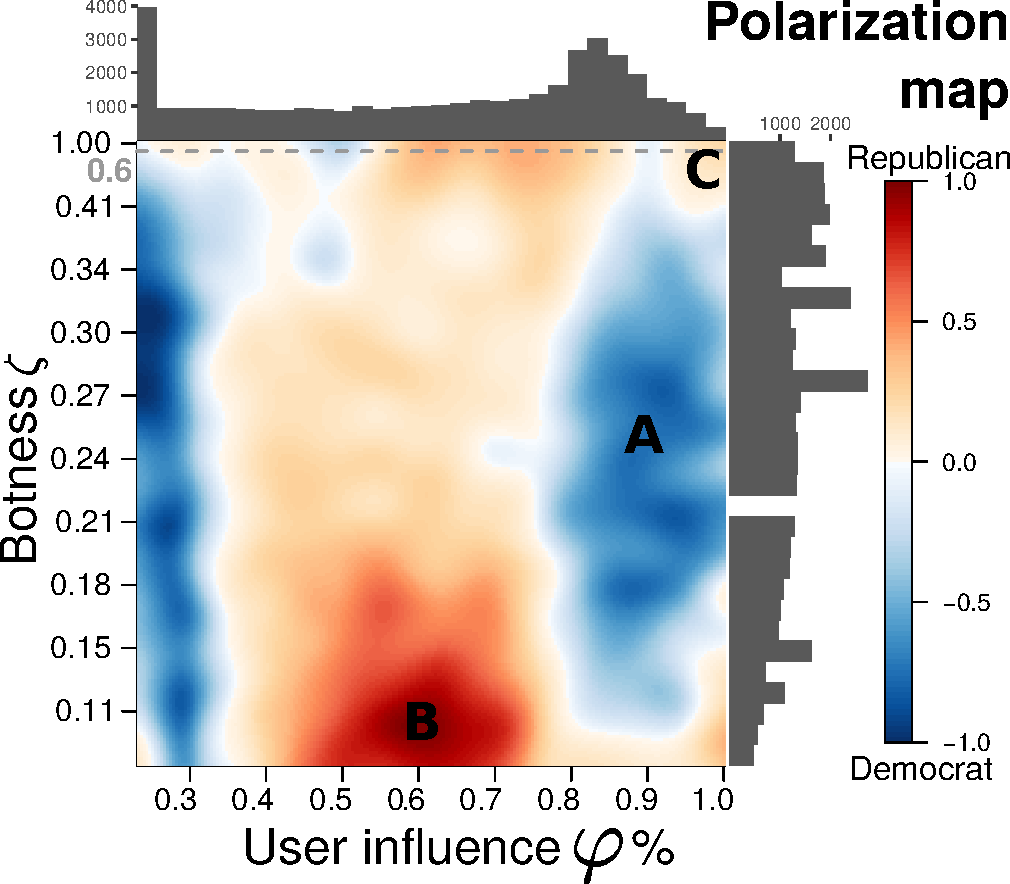
\includegraphics[width=0.47\textwidth]{influence-botscore-polarization-2d-map}

	\caption{ 
		Political polarization by user influence $\varphi(u) \%$ (x-axis) and bot score $\zeta$ (y-axis).
%		The x-axis shows the percentile of user influence, from 0 being the least influential to 1 being the most influential.
%		The y-axis shows the bot score. 
		% (see the distribution of bot score density in Fig.~\ref{subfig:botscore-density}).
		The gray dashed horizontal line shows the threshold of 0.6 above which a user is considered a bot.
		The color in the map shows political polarization: areas colored in bright blue (red) are areas where the Democrats (Republicans) have considerably higher density than Republicans (Democrats).
		%: it is the ratio of the density of Democrat users to the density of Republican users.
%		Areas where the density of Republicans is considerably higher than the density of Democrats are colored bright red (and similarly for bright blue).
		Areas where the two populations have similar densities are colored white.
		Three areas of interest are shown by the letter \textbf{A}, \textbf{B} and \textbf{C}.
	}
	\label{fig:polarization-map}
%	\captionmoveup
\end{figure}

\subsection{User influence and polarization map}
\label{subsec:user-influence-results}

\textbf{User influence across four populations.}
First, we study the distribution of user influence across the four reference populations constructed in Sec.~\ref{subsec:bot-detection}.
We plot the CCDF in Fig.~\ref{subfig:user-infl-CCDF} and we summarize user influence as boxplots in Fig.~\ref{subfig:user-infl-boxplots} for each population.
User influence $\varphi$ is long-tail distributed (shown in Fig.~\ref{subfig:user-infl-CCDF}) and it is higher for \Bot and \Suspended populations, than for \Human and \Protected (shown in Fig~\ref{subfig:user-infl-boxplots}).
There is a large discrepancy between the influence of \Human and \Bot (p-val $= 0.0025$), with \emph{the average bot having 2.5 times more influence than the average human.}
%\TODO{MAR}{Message in text: bots have higher user influence.}
We further break down users in the \Bot population based on their political polarization.
Fig.~\ref{subfig:bot-influence} aggregates as boxplots the influence of pro-Democrat and pro-Republican bots (note: not all bots are politically polarized).
Notably, on a per-bot basis, pro-Republican bots are more influential than their pro-Democrat counterparts (p-val $= 0.0096$) -- \emph{the average pro-Republican bot is twice as influential as the average pro-Democrat bot}.
%\TODO{MAR}{Message in text: republican bots are more influential than democratic bots.}

\textbf{Political polarization and user influence.}
Next, we analyze the relation between influence and polarization.
Fig.~\ref{subfig:polarization-conditioned-user-infl} plots the probability distribution of political polarization, conditioned on user influence $\varphi \%$.
While for mid-range influential users ($\varphi \% \in [0.4, 0.8]$) the likelihood of being Republican is higher than being Democrat, we observe the inverse situation on the higher end of the influence scale.
\emph{Very highly influential users ($\varphi \% > 0.8]$) are more likely to be pro-Democrat}, and this is consistent with the fact that many public figures were supportive of the Democrat candidate during the presidential campaign.
%\TODO{MAR}{Message in text: highly influential users are likely to be democrats -- mobilization of civil society.}

\textbf{The polarization map.}
Finally, we create a visualization that allows us to jointly account for botness and user influence when studying political partisanship.
We project each politically polarized user in \debate onto the two-dimensional space of user influence $\varphi \%$ (x-axis) and botness $\zeta$ (y-axis).
The y-axis is re-scaled so that an equal length interval around any botness value contains the same amount of users,
This allows to zoom in into denser areas like $\zeta \in [0.2, 0.4]$, and to deal with data sparsity around high botness scores.
We compute the 2D density estimates for the pro-Democrat and pro-Republican users (shown in the online supplement~\cite[annex~E]{supplemental}).
%\ref{si-sec:polarization-map}
%While these allow to identify dense and sparse regions, for one polarization or the other, in order to show both 
For each point in the space $(\varphi \%, \zeta)$ we compute a score as the log of the ratio between the density of the Republican users and that of the pro-Democrats, which is then renormalized so that values range from -1 (mostly Democrat) to +1 (mostly Republican).
The resulting map -- dubbed the \emph{polarization map} -- is shown in Fig.~\ref{fig:polarization-map} and it provides a number of insights.
Three areas of interest (\textbf{A}, \textbf{B} and \textbf{C}) are shown on Fig.~\ref{fig:polarization-map}.
Area \textbf{A} is a pro-Democrat area corresponding to highly influential users (already shown in Fig.~\ref{subfig:polarization-conditioned-user-infl}) that spans across most of the range of botness values.
Area \textbf{B} is the largest predominantly pro-Republican area and it corresponds to mid-range influence (also shown in Fig.~\ref{subfig:polarization-conditioned-user-infl}) and concentrates around small botness values -- this indicates the presence of a large pro-Republican population of mainly human users with regular user influence.
Lastly, we observe that the top-right area \textbf{C} (high botness and high influence) is predominantly red: 
%are more likely to be \rvt{pro-Republican}.
In other words \emph{highly influential bots are mostly pro-Republican.}

%!TEX root = main.tex

\section{Discussion}
 
In this paper, we study the influence and the political behavior of socialbots.
We introduce a novel algorithm for estimating user influence from retweet cascades in which the diffusion structure is not observed.
%-based  under conditions of incomplete data. Twitter does not provide retweet structures in its data, and simply associates all retweets with the original tweet. 
%As a result, this obscures crucial information about social communication on the platform, potentially leading to incorrect analyses of retweet activity. 
%We model the latent diffusion structure using only tweeting time and user features and implemented a scalable algorithm to estimate user influence over all possible diffusion scenarios.
We propose four measures
%We apply it 
to analyze the role and user influence of bots versus humans on Twitter during the 1st U.S. presidential debate of 2016. 
The first is the user influence, computed over all possible unfoldings of each cascade.
%The dataset comprised 6,498,818 tweets emitted by 1,451,388 users over a 2-hour duration, containing 200,191 retweet diffusion cascades of size 3 or greater. 
Second, we use the BotOrNot API to retrieve the botness score for a large number of Twitter users.
% $\zeta(u) \in [0, 1]$ (0 being likely human, and 1 likely non-human). 
Lastly, by examining the 1000 most frequently-used hashtags we measure political polarization and engagement. 
We analyze the interplay of influence, botness and political polarization using a two-dimensional map -- the polarization map.
We make several novel findings, for example: bots are more likely to be pro-Republican; the average pro-Republican bot is twice as influential as its pro-Democrat counterpart; very highly influential users are more likely to be pro-Democrat; and highly influential bots are mostly pro-Republican.

%7/ I see a need to discuss the algorithm (and model) behind BotOrNot API, because: 
%
%an alternative explanation for claims below (intro page 2)
%> ** bots are more engaged than humans
%> * bots are more likely to be pro-Republican;
%
%
%
%can be: 
%** the API tend to flag more “engaged” account as bots 
%* if the API uses the same def about republican, e.g. set of keywords (or accidentally use something like network connectivity to a set of known republicans who uses the same hashtags that Tim identified … 
%
%to sum up, this is a tough chicken-n-egg question. 
%it is similar to saying some API flagged a person as “should not allow bail” but it had race as input and the person scored high on that (!)
\textbf{Validity of analysis with respect to BotOrNot.}
The BotOrNot algorithm uses tweet content and user activity patterns to predict botness.
%The results presented in Sec.\ref{sec:results-findings} are not simply due to cofounding 
However, this does not confound the conclusions presented in Sec.~\ref{sec:results-findings}.
First, political behavior (polarization and engagement) is computed from a list of hashtags specific to \debate, while the BotOrNot predictor was trained before the elections took place and it has no knowledge of the hashtags used during the debate.
Second, a loose relation between political engagement and activity patterns could be made, however we argue that engagement is the number of used partisan hashtags, not tweets -- i.e. users can have a high political engagement score after emitting few very polarized tweets.

\textbf{Assumptions, limitations and future work.}
This work makes a number of simplifying assumptions, some of which can be addressed in future work.
First, the delay between the tweet crawling (Sept 2016) and computing botness (July 2017) means that a significant number of users were suspended or deleted.
A future application could see simultaneous tweets and botscore crawling.
Second, our binary hashtag partisanship characterization does not account for independent voters or other spectra of democratic participation, and future work could evaluate our approach against a clustering approach using follower ties to political actors \cite{barbera.2015}.
Last, this work computes the expected influence of users in a particular population, but it does not account for the aggregate influence of the population as a whole.
Future work could generalize our approach to entire populations, which would allow answers to questions like ``Overall, were the Republican bots more influential than the Democrat humans?''.

%To conclude, this paper makes an important and novel contribution to the problem of estimating influence in retweet cascades. 
%Furthermore, our case study application of this approach to studying bot influence during the U.S. election provides shows that this approach can elicit fundamentally new, and indeed surprising, insights about power and influence in social media platforms such as Twitter. 
%We note several limitations to this work and suggest areas of future research. \TODO{@MAR}{Technical limitations?}. The application of our method to study bot influence during the 2016 U.S. political election is limited by the time range of tweet activity (90 minutes during the 1st presidential debate and 15 minutes before and after). Further, whilst we managed to classify every user in the dataset using the BotOrNot API, the delay between the Debate and our classification meant that a significant number of users were suspended or deleted. Although we accounted for this in the analysis, the presence of these users is a limiting factor in the findings. The algorithm presented in this paper and its application suggests several key directions for future research. Firstly, \TODO{@MAR}{technical future work?}. 
%
%Secondly, \TODO{@ROB}{we present a somewhat simplistic binary characterization of political partisanship that does not, for example, account for independent voters or other spectra of democratic participation. Future work could compare \textbf{TO DO}}. Finally, analysis of a larger dataset of political discussions on Twitter is necessary to verify the empirical results we obtained and test how these generalise more broadly to the political context not only in the US but in other contexts. 

\vspace{0.2cm}
\noindent{%\small
\textbf{Acknowledgments.}
This research is sponsored in part by the Air Force Research Laboratory, under agreement number FA2386-15-1-4018.
%We thank the National Computational Infrastructure (NCI) for providing computational resources, supported by the Australian Government.
}

{ %\small
\fontsize{9.0pt}{10.0pt}
%\fontsize{9.5pt}{10.5pt}
\selectfont
\bibliography{paper}
\bibliographystyle{aaai}
}

%!TEX root = main.tex
%
\newpage
\appendix
%
\etocdepthtag.toc{mtappendix}
\etocsettagdepth{mtchapter}{none}
\etocsettagdepth{mtappendix}{subsection}
\etoctocstyle{1}{Contents (Appendix)}
\tableofcontents

\section{Derivation of the influence formula}
\label{si-sec:infl-derivation}

In this section, we detail the calculation of the tweet influence $\varphi(v)$, proposed in Sec.~\ref{sec:user-influence}.
%We start from an observed retweet cascade, for which the Twitter API does not provide the actual structure of the social network.
In Sec.~\ref{subsec:diffusion-scenario}, we define the notion of diffusion scenario, and we compute its likelihood given an observed retweet cascade.
In Sec.~\ref{subsec:user-influence}, we compute the formula for tweet influence over all possible diffusion scenarios associated with the given cascade.

\subsection{Diffusion scenarios}
\label{subsec:diffusion-scenario}

\textbf{Diffusion trees.}
We can represent an online diffusion using a directed tree $G(V, E)$, in which each node has a single parent and the direction of the edges indicates the flow of the information.
For retweet cascades, the nodes $v \in V$ are individual tweets and each directed edge $e \in E, e = \{v_a, v_b\}$ (showing the direction $v_a \longrightarrow v_b$) indicates that $v_b$ is a \emph{direct retweet} of $v_a$.
A direct retweet means that $u_b$ -- the user that emitted the tweet $v_b$ -- clicked on the ``Retweet'' option under tweet $v_a$.
The top panel of Fig.~\ref{fig:example-diffusion-graph-construction} shows an example of such a diffusion tree.
Note that each node $v$ has associated a time of arrival $t_v$ and that the diffusion tree respects the order of the times of arrival -- i.e. given the edge $e = \{v_a, v_b\}$, then $t_a < t_b$.
The bottom panel of Fig.~\ref{fig:example-diffusion-graph-construction} shows the incremental construction of the diffusion tree shown in top panel:
node $v_1$ is the root of the tree and the source of the information diffusion; 
at each time $t_i$, node $v_i$ attaches to the previous tree constructed at time $t_{i-1}$.

%We start from the graph representation of a social network, in which nodes correspond to users and the directed edges correspond to social ties -- following the updates of another user on Facebook, the following relation on Twitter etc.
%We can represent the diffusion of information in a social graph as a directed tree (as shown in Fig.~\ref{fig:example-diffusion-graph}).
%Fig.~\ref{fig:diffusion-graph-construction} shows the associated diffusion process:
%leaves attach to the tree sequentially, as the information propagation progresses.
%%the propagation process continues by sequentially attaching new leaves to this tree over time as shown in Fig.~\ref{fig:diffusion-graph-construction}.

%!TEX root = paper.tex

\begin{table}[!b]
%\caption{Summary of notations and parameters in the paper, together with their interpretation. These notations are superscripted by $w$ when referring to cascade $w$ -- e.g. $\hat N_\infty^w$.}
\caption{Summary of notations.}
\small
\centering
\begin{tabular}{cp{5.5cm}}
\toprule
Notation & Interpretation \\ %\textbf{Significance and usage} \\ 
\midrule
	$G(V, E)$ & diffusion tree. In case the tree is unobserved, $G$ is a diffusion scenario. \\ 
	$v \in V$ & node in the diffusion tree (i.e. retweets). \\ 
%$\mu(t)$ & external events arrival rate. \\ 
%\parbox[c]{1.4cm}{$e \in E$,\\ $e = \{a, b\}$} 
% \begin{minipage}[c]{1.4cm}
%  $e \in E$, $e = \{a, b\}$
% \end{minipage} 
	$e = (v_a, v_b) \in E$ & directed edge in the diffusion tree, tweet $v_b$ is a direct retweet of $v_a$.\\
	$t_v$ & time of arrival of node $v$ (timestamp of the tweet). \\
	$u_v$ & user that has emitted tweet $v$. \\
	$m_v$ & local influence (i.e. number of followers) of user $u_v$. \\
\bottomrule
\end{tabular}
\label{tab:parameters}
%\captionmoveup
\end{table}


\begin{figure*}[tbp]
	\newcommand\mywidth{0.5}
	\newcommand\myheight{0.2}
	\centering
	
	\subfloat[] {
		\begin{tabular}{c}
			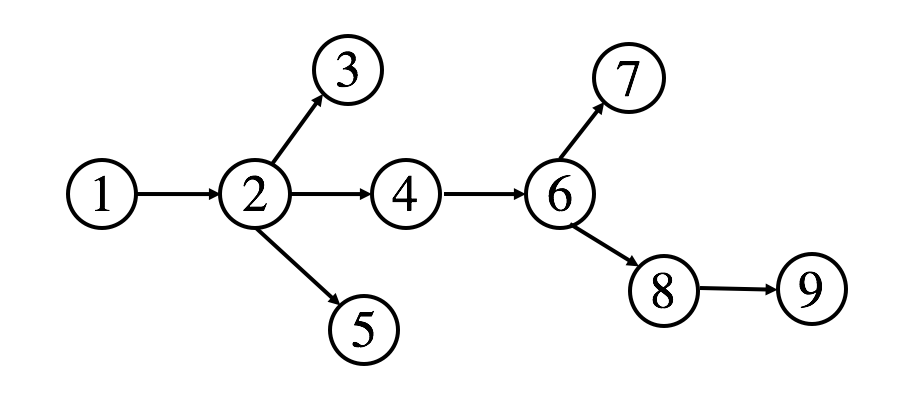
\includegraphics[width=0.32\textwidth,valign=c]{diffgraph} \\
			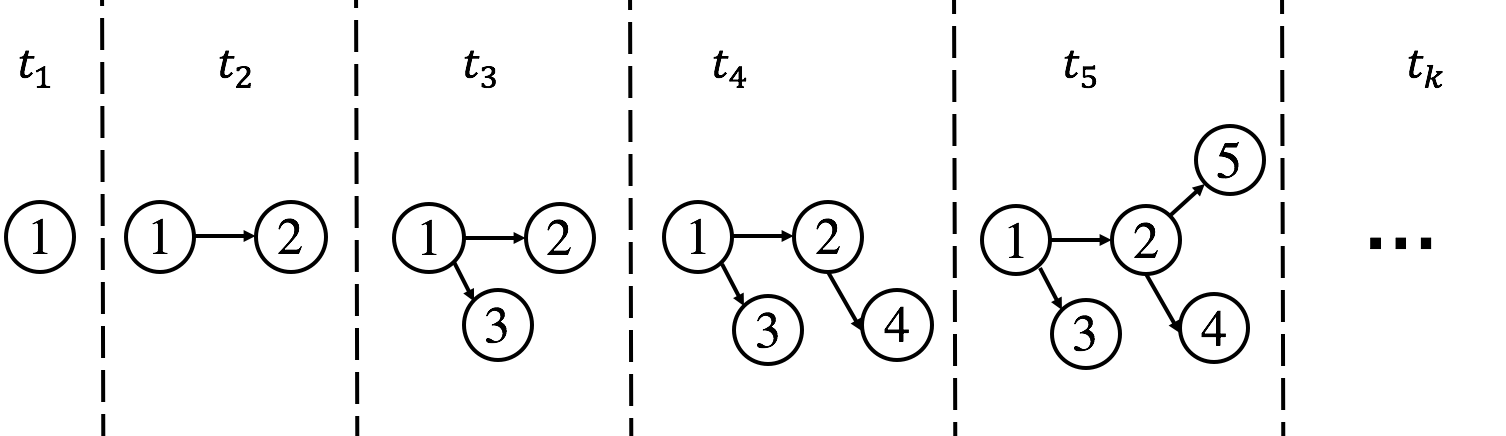
\includegraphics[width=0.51\textwidth,valign=c]{onediff}
		\end{tabular}
		\label{fig:example-diffusion-graph-construction}
	}
	\subfloat[] {
			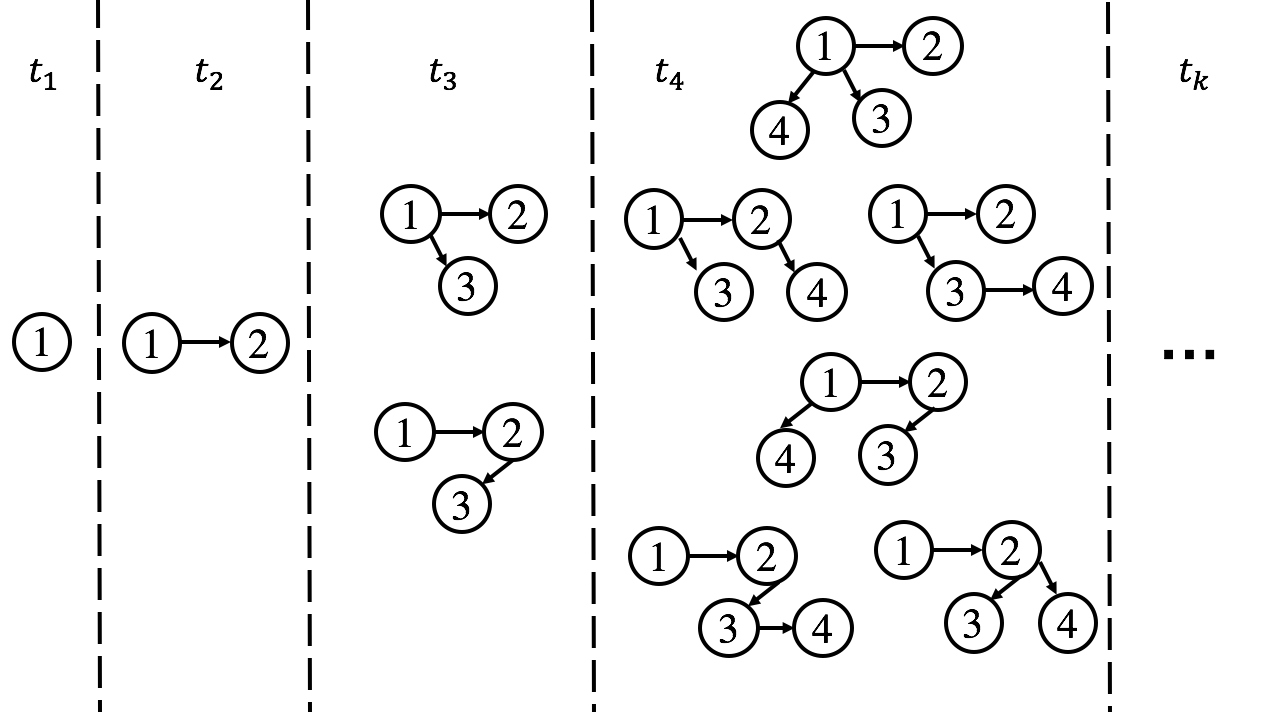
\includegraphics[height=0.2\textheight,valign=c]{diffusion}
			\vphantom{ % MAR: this is here to keep the label at the same position as for the other figures.
				\begin{tabular}{c}
					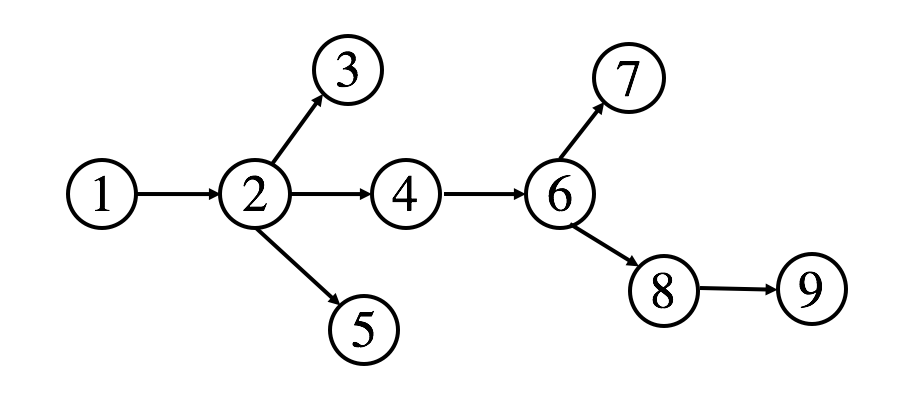
\includegraphics[width=0.32\textwidth,valign=c]{diffgraph} \\
					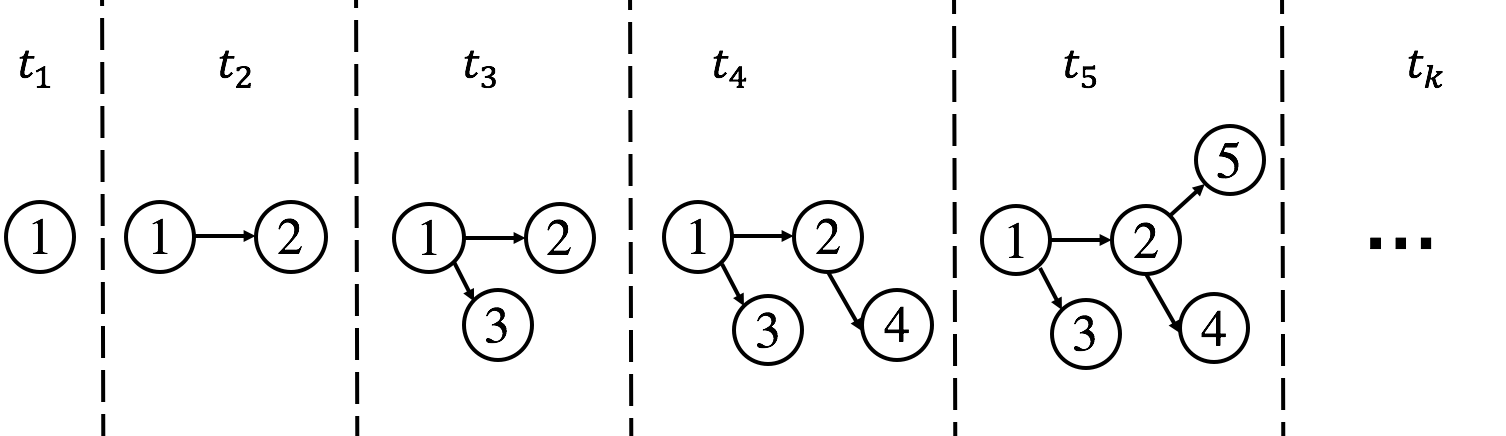
\includegraphics[width=0.51\textwidth,valign=c]{onediff}
				\end{tabular}
			}
			\label{fig:diffusion-scenarios} 
		}	
	
%	\begin{tabular}{cc}
%		\subfloat[] {
%			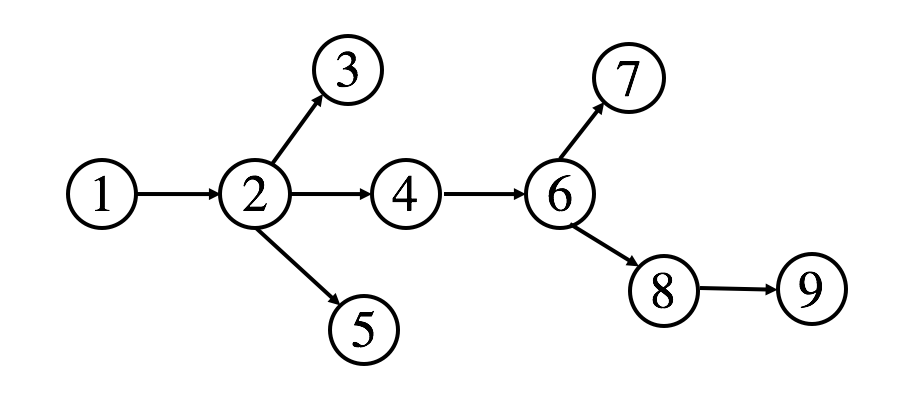
\includegraphics[width=0.32\textwidth,valign=c]{diffgraph}
%			\label{fig:example-diffusion-graph}
%	} &
%		\multirow{2}{*}[2em]{\subfloat[] {
%			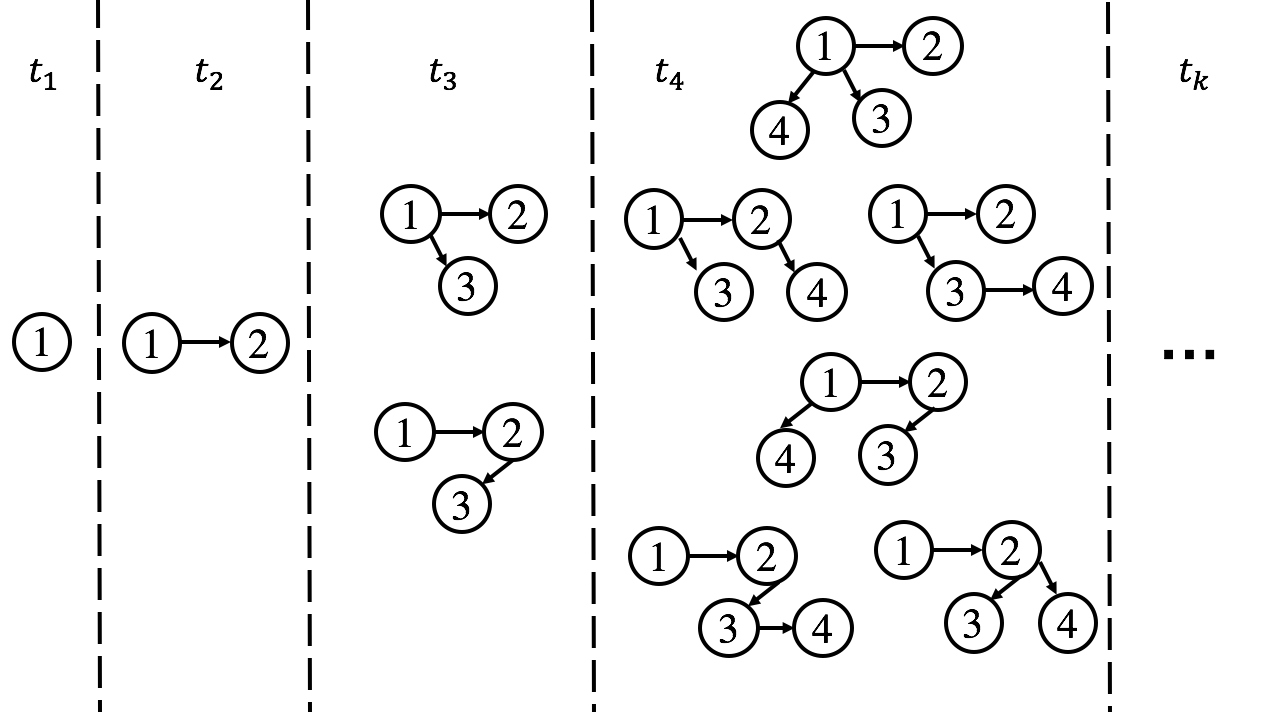
\includegraphics[height=0.2\textheight,valign=c]{diffusion}
%			\label{fig:diffusion-scenarios} 
%		}} \\
%	
%	%% new row	
%	\subfloat[] {
%		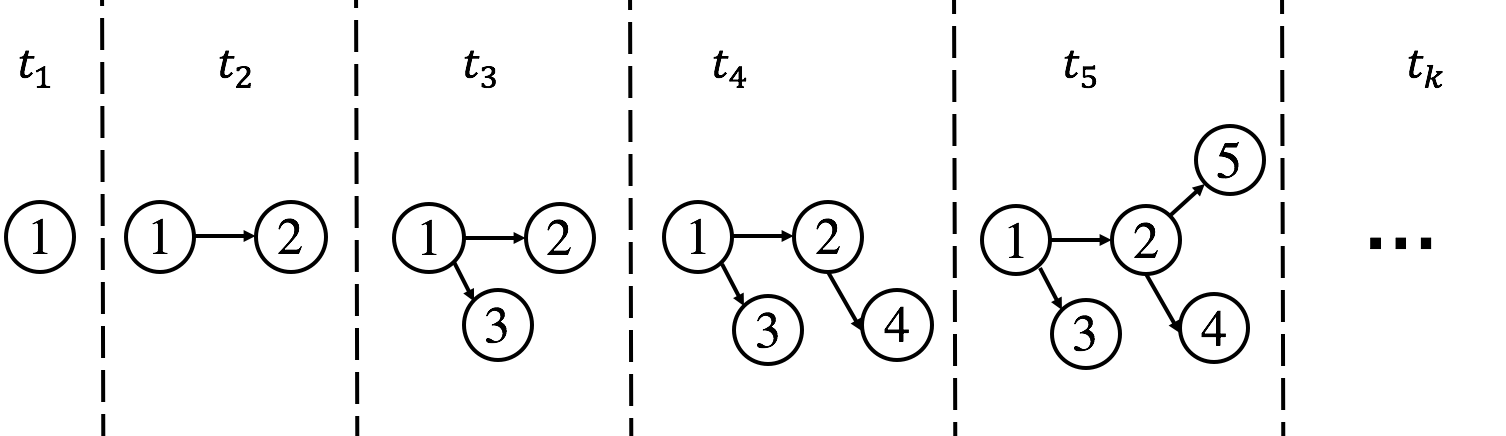
\includegraphics[width=0.51\textwidth,valign=c]{onediff}
%		\label{fig:diffusion-graph-construction}
%	} & \\
%	\end{tabular}



%	\subfloat[] {
%		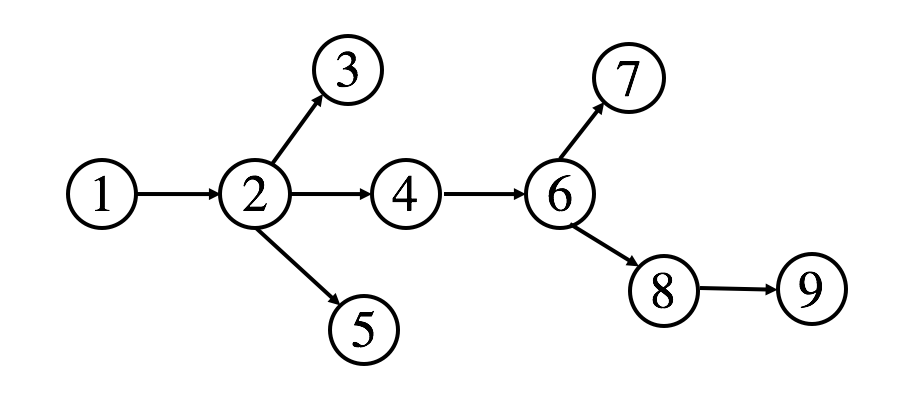
\includegraphics[width=\mywidth\textwidth,valign=c]{diffgraph}
%		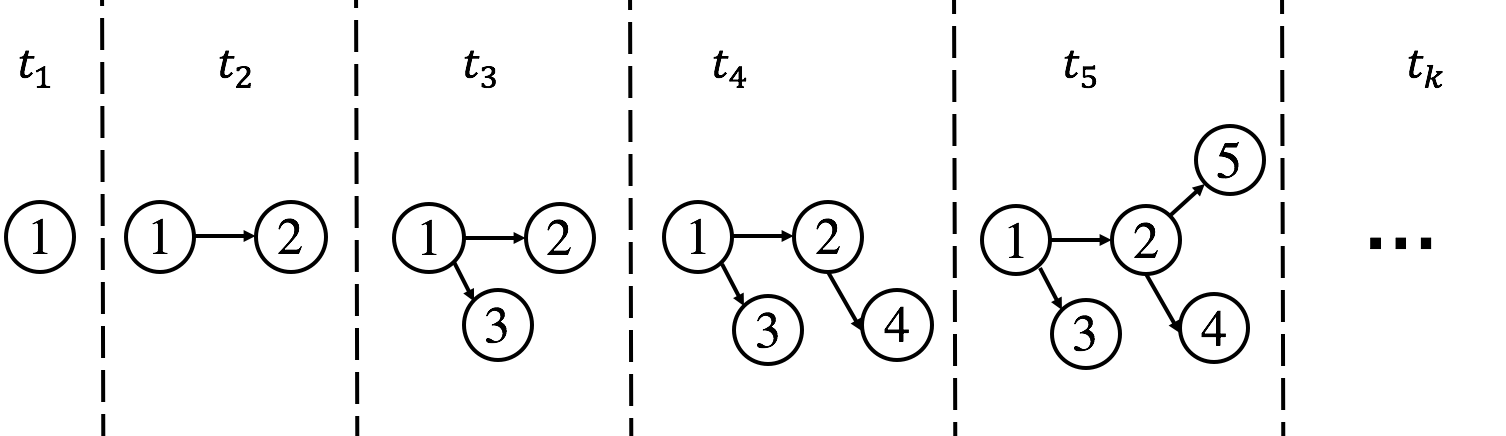
\includegraphics[width=\mywidth\textwidth,valign=c]{onediff}
%		\vphantom{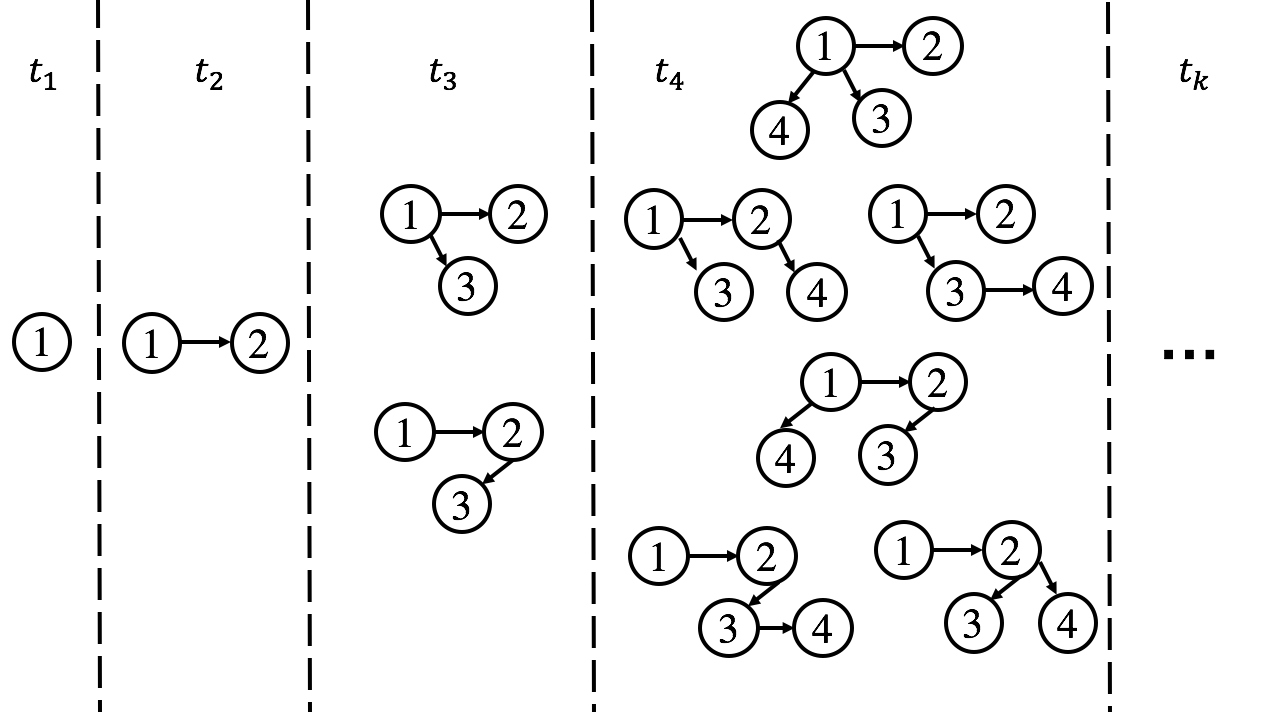
\includegraphics[height=\myheight\textheight,valign=c]{diffusion}}% MAR: this is here to keep the label at the same position as for the other figures.
%		\label{fig:side:a}
%	}
%	\hspace{0.2cm}
%	\subfloat[] {
%		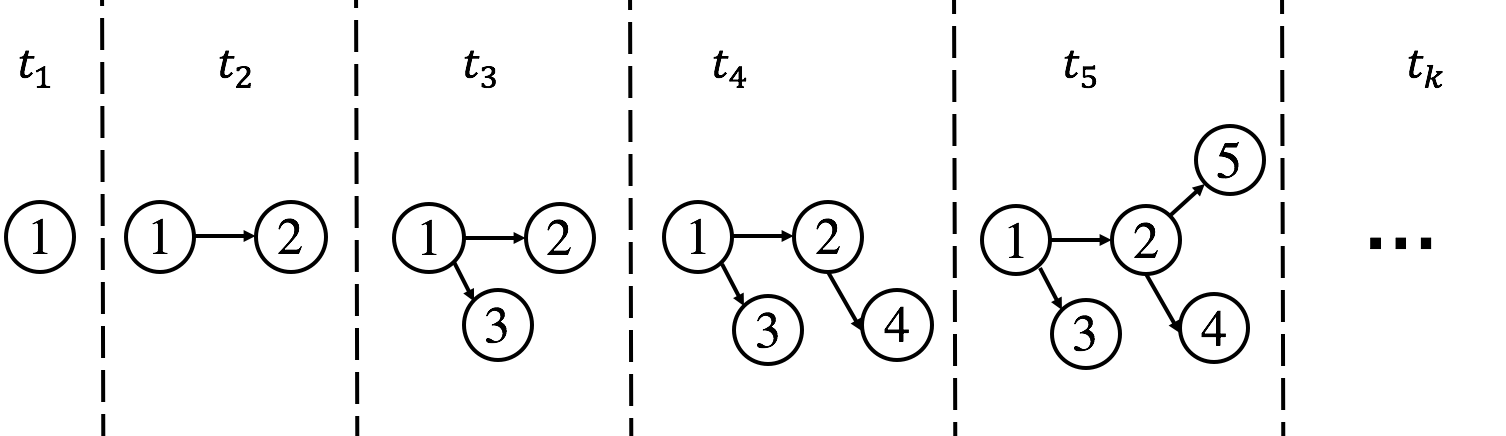
\includegraphics[width=\mywidth\textwidth,valign=c]{onediff}
%		\vphantom{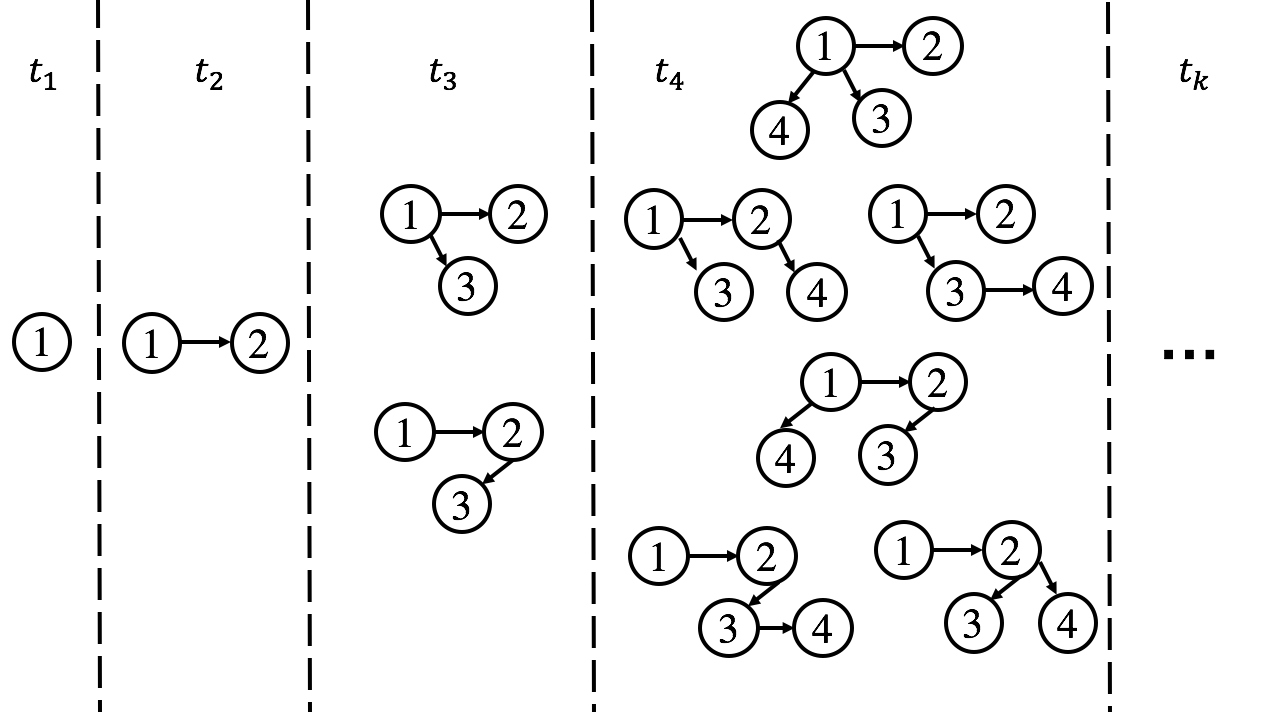
\includegraphics[height=\myheight\textheight,valign=c]{diffusion}}% MAR: this is here to keep the label at the same position as for the other figures.
%		\label{fig:side:b}
%	}
%	\hspace{0.2cm}
%	\subfloat[] {
%		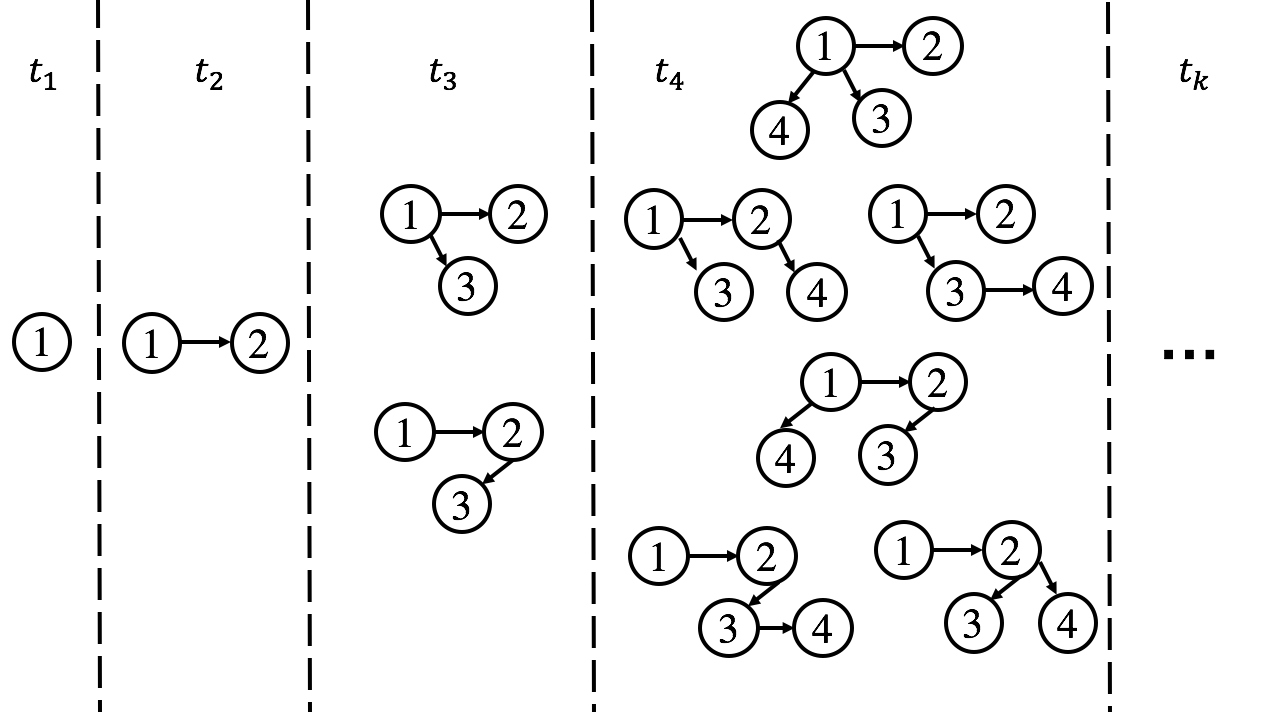
\includegraphics[height=\myheight\textheight,valign=c]{diffusion}
%		\label{fig:diffusion-scenarios}
%	}
	\caption{
		\textbf{(a)} An example of a diffusion tree \textbf{(top)} and its corresponding incremental diffusion process \textbf{(bottom)}.
		\textbf{(b)} Enumeration of all possible diffusion scenarios: 
		each retweet $v_k$ arrives at time $t_k$, and it can attach to any of the previous nodes, in any of the diffusion scenario constructed at time $t_{k-1}$.
		At time $t_k$ there are $(k-1)!$ diffusion scenarios, each with $k$ nodes.
	}
%	\captionmoveup
\end{figure*}

\textbf{Diffusion scenarios for retweet cascades.}
The diffusion tree is not observed for real Twitter retweet cascades, since the Twitter API does not expose the direct retweet relationships.
Instead, it assigns every retweet in the cascade to the original tweet.
%
%The underlying social graph is not observed for real Twitter retweet diffusions. 
%For data availability reasons, we only observe the order and timing of arrival of nodes.
%The Twitter API assigns every retweet to the original tweets, regardless of any retweeting chains.
%Consequently, 
Every retweet cascades constructed based on raw retweet information from the Twitter API resembles the graph in Fig.~\ref{fig:side:a}.
Due to this particular shape, we denote retweet cascades as \emph{stars}.
However, the API exposes the time of arrival of the retweets $t_i$.
We denote as a \emph{diffusion scenario} any valid diffusion tree that could be associated with the observed retweet star -- i.e., the edges in the diffusion tree respects the order of arrival of retweets.
%
%We denote the valid diffusion trees that could generate an observed star as \emph{diffusion scenarios}.
Fig.~\ref{fig:side:b} shows four examples of diffusion scenarios associated with the star in Fig.~\ref{fig:side:a}.
%Since we only observe the times when certain node are added through diffusion process, there are many possible diffusion scenarios that explain a observed cascades Fig.~\ref{fig:side:a} and .

%A diffusion scenario can be regarded as one of these tree. 

\textbf{Constructing diffusion scenarios.}
%All possible diffusion scenarios need to be constructed. 
Fig.~\ref{fig:diffusion-scenarios} exemplifies a straight-forward method to enumerate all diffusion scenarios associated with the star in Fig.~\ref{fig:side:a}.
The node $v_1$ is the root node and it is published at time $t_1$;
tweet $v_2$ occurs at time $t_2$ and it is undoubtedly a direct retweet of $v_1$ -- a directed edge is drawn from $v_1$ to $v_2$. 
Tweet $v_3$ observed at $t_3$ can be a direct retweet of either tweet $v_1$ or tweet $v_2$.
Therefore, at time $t_3$ there are two possible diffusion scenarios: 
$G_1$ with the edge set $E = \lbrace \{v_1, v_2\}, \{v_1, v_3\} \rbrace$ and $G_2$ with the edge set $E = \lbrace \{v_1, v_2\}, \{v_2, v_3\} \rbrace$.
Similarly, $v_4$ can be a direct retweet of $v_1$, $v_2$ or $v_3$, in either $G_1$ or $G_2$.
Consequently, at time $t_4$ there are 6 possible diffusion scenarios.
The process continues until all nodes have been attached.
For an observed star of size $k$, there are $(k-1)!$ associated diffusion scenarios.
%Then two directed edges are drawn from $u_1$ to $u_3$ and $u_2$ to $u_3$. 
%Thus, two diffusion scenarios $G_1$ and $G_2$ are constructed due to the different users to retweet. 
%When the fourth user appears, it can retweet from $u_1$ to $u_3$ in any of previous diffusion scenarios. 
%This process will continue till the last user we observe. 
%Then All possible diffusion scenarios are built by sequentially adding users to previous diffusion scenarios.
%Eventually $(k-1)!$ number of diffusion scenarios are constructed when a cascade with the size of $k$ is observed.

\textbf{Probability of a diffusion scenario.}
%We denote as $v_i$ the user that has emitted the tweet $i$.
Given that in retweet cascades individual edges are not observed,
%Given that edges in diffusion scenarios are not observed,
%For diffusion scenarios, the edges (i.e. the direct retweet events) are not observed.
we define the probability of an edge $\mathds{P}(\{v_a, v_b\})$ as the likelihood that $u_b$ emitted tweet $v_b$ as a direct retweet of $v_a$.
%In line with previous work~\cite{crane2008robust,Mishra2016,Zhao2015,Shen2014,Yu2015},
We model two factors in the likelihood of retweeting:
%
%To estimate user influence. 
%Only obtaining all the possible diffusions scenarios is not enough. 
%Given a possible diffusion scenario $G$, we also need to know the probability of retweeting which corresponding to the weight of each edge in $G$. 
%More specifically, 
%
%Every edge $e$ correspond to a value representing the probability of retweeting. 
%To model this probability, 
%We model the probability of an edge using two assumptions: 
firstly, users retweet \emph{fresh} content~\cite{Wu2007}.
The probability of the edge $e$ decays exponentially with the time difference $t_b - t_a$;
%The influence of user is exponential decay
secondly, users prefer to retweet locally influential users, also known as preferential attachment~\cite{Barabasi2005}.
We measure the local influence of a user using his number of followers~\cite{kwak2010twitter,Cha2010,Rizoiu2017}.
%The second assumption is that user prefers retweet from a user who has a lot of followers. 
%The number of followers a user has often related to its number of retweet. 
%More followers, a user has more channels he can get to broadcast his tweet to others, which increasing the likelihood of seeing by other users~\cite{1,2}.
%So the probability of retweeting can be express in the following equation:
We quantify the probability of an edge as:
\begin{equation} \label{eq:prob-edge}
	\mathds{P}(\{v_a, v_b\}) = m_a e^{-r({t_{b}-t_{a}})}
\end{equation}
%This equation describe the probability that user $u_b$ retweet from user $u_a$ 
where 
%$t_a$ and $t_b$ represent the retweet time of $u_a$ and $u_b$ respectively;
$m_a$ is the number of followers of the user of $u_a$ and
$r$ controls the temporal decay of the probability.
%$e^{-r({t_{b}-t_{a}})}$ express the probability decrease in exponential.
%$G$ is one diffusion scenario which user $u_b$ is added to.
%The probability of a diffusion scenario is intimately linked to the probability of an edge.

Under the assumption that retweeting events (i.e. edges) occur independently one from another, we obtain the probability of a diffusion scenario as:
%
%\textbf{Probability of diffusion scenarios.}
%As we describe above, one diffusion is constructed by a sequence of retweeting edges. 
%Each user $u_b$ will retweet from another user $u_a$ in its parent scenario with probability $\mathds{P}(u_a,u_b)$. 
%As each rewteet represent an egde $e$ in diffusion scenario.Thus, we can obtain the probability of a diffusion scenarios $\mathds{P}(G)$ via:
\begin{equation} \label{eq:prob-scenario}
	\mathds{P}(G) = \prod_{\{v_a,v_b\} \in E} \mathds{P}(\{v_a, v_b\})
\end{equation}

Note that the above assumption of independence of retweet events is a strong assumption.
Current state-of-the-art approaches~\cite{Mishra2016,Zhao2015} for modeling retweet cascades employ self-exciting point processes, in which the arrival of one event increases the probability of future events.
However, for our application of estimating the probability of a diffusion scenario it is the simplest assumption.
Additional arguments in its favor are also that we are studying networks of events
%\verify{RJA comment: Re. above assumption that retweeting events are independent of one another: it could be emphasised here that this assumption is valid because we are studying retweet cascades i.e. it is a network of events 
(in which each event is identified with unique user), not networks of users. 
The interdependence often observed in socially generated networks (like triadic closure)
%e.g. reciprocity, triangles by construction 
can be ignored in edge formation within a particular retweet cascade. 
%It's a directed acyclic graph (if I've got the right term?)}

\subsection{Computing tweet influence}
\label{subsec:user-influence}

\cite{Du2013} define user influence of a user $u$ as the average number of users in the social network who get in contact with the content emitted by $u$.
For retweet cascades the diffusion tree is not observed; it is impossible to directly measure user influence, apart from the root user.
We define the \emph{tweet influence} over a retweet cascade as the expected number of time it is retweeted -- direct retweets or descendants in a diffusion scenario --, over all possible diffusion scenarios associated with the given star.
Finally, we compute the influence of user $u$ as the sum of the influences of the tweets that $u$ authored.
We see that the definition in~\cite{Du2013} is a special case of our definition, in which the diffusion tree is observed.

\textbf{Tweet influence over one diffusion scenario.}
%Intuitively, given a diffusion scenarios G, the wider the spreading tweet, the more influential the user.
%We adopt the definition of influence as the number of average users that a target user can diffuse tweet to as in the previous work~\cite{3}.
%More precisely, let's say $U$ is the collection of users in G.
%
Let $z(v_i, v_k) \in G$ be a path in the diffusion scenario $G$ -- i.e a sequence of nodes which starts with $v_i$ and ends with $v_k$.
$\varphi(v_i | G)$ is the influence of $v_i$ given the diffusion scenario $G$ and it is computed as number of users reached from $v_i$ i.e. the number of descendants of $v_i$.
%, and $\varphi$ would be the  using a model of independent binomials to decide whether or not to take each hop in the path (instead of average number of reachable users … unclear what it means)
Formally:
%
%Consider a target user $v_i \in U$.
%This $v_i$ can diffuse its tweet to any user $v_k \in U $ though the path $z(v_i,v_k)$ which is from $v_i$ to $v_k$.
%The expected number of diffused user given a target user $v_i$ can be computed as: 
\begin{equation}
	\varphi(v_i|G) 	=  \sum_{v_k \in V(G)} \mathds{1} \{z(v_i,v_k | G) \} \label{eq:infl-in-a-scenario}
\end{equation}
where $\mathds{1} \left\lbrace z(v_i,v_k|G) \right\rbrace$ is a function that takes the value 1 when the path from $v_i$ to $v_k$ exists in $G$.
%and the probability of path $z(v_i,v_k|G)$ can be obtained by the production over edges in this path $z$. That is:
%\begin{equation}
%	\mathds{P} \big(z(v_i,v_k|G) \big) = \prod_{\{u_a,u_b\} \in z} \mathds{P}\big(\{u_a,u_b\}\big).
%\end{equation}

\textbf{Tweet influence over a retweet cascade.}
We compute the influence of tweet $v_i$ over $VG$ -- all possible diffusion scenarios associated with a retweet cascade -- as:
%Since we do not have only one diffusion scenarios.
%We have multiple diffusion scenarios. 
%So the influence of target user  $\varphi(v_i)$ can be express as summing out $\varphi(v_i|G)$ over all possible diffusion scenarios:
\begin{align}
	\varphi(v_i) 	&= \sum_{G\in{VG}} \mathds{P}(G) \varphi(v_i|G) \nonumber \\
				&= \sum_{G\in{VG}} \mathds{P}(G) \sum_{v_k \in V(G)} \mathds{1}\big( z(v_i,v_k|G) \big) \label{eq:brute-user-infl}
\end{align}
%Where $VG$ is the collection of all possible diffusion scenarios that are generated from an observed retweet cascade. $G$ is one possible diffusion scenario in $VG$. The final user influence over all possible diffusion scenarios is:
%\begin{equation} \label{eq:user-infl-definition}
%\varphi(u) = \sum_{G\in{VG}}\mathds{P}\{G\} \sum_{u \in G}\prod_{\{u_a,u_b\} \in z}\frac{f(u_a)}{\sum_{u\in {G}}f(u)}e^{-r({t_{b}-t_{a}})}
%\end{equation}
It is intractable to directly evaluate Eq.~\eqref{eq:brute-user-infl}, plugged in with Eq.~\eqref{eq:prob-scenario} and~\eqref{eq:infl-in-a-scenario}, particularly due to the factorial number of diffusion scenarios in $VG$.
%It is challenging to compute Eq.~\eqref{eq:user-infl-definition} directly, particularly given that the number of diffusion scenarios is factorial with the size of diffusion cascade.
For example, there are $10^{156}$ diffusion scenarios for a cascade of 100 retweet.
We develop, in the next section, an efficient linear time algorithm to compute the influence of all tweets in a retweet cascade.
%To solve this problem, we develop an efficient algorithm in the next section.

\section{Efficient tweet influence computation}
\label{si-sec:efficient-algo}

The key observation is that each tweet $v_k$ is added simultaneously at time $t_k$ to all diffusion scenarios constructed at time $t_{k-1}$.
$v_k$ contributes only once to the tweet influence of each tweet that is found on the branch it attached to.
This process is exemplified in Fig.~\ref{fig:add-one-edge}.
Node $v_5$ is added to a given diffusion scenario, generating 4 new diffusion scenarios at time $t_5$.
We color in red the nodes whose influence increases as a result of adding node $v_5$.
%
%The key observation to efficiently compute user influence is that users $v_k$ are sequentially added to the diffusion scenarios constructed at time $t_k$. 
%If we ignore $v_k$, the structure of all previous diffusion scenarios remains unchanged. 
This allows to compute the tweet influence incrementally, by updating $\varphi(v_i), i < k$ at each time $t_k$.
We denote by $\varphi^k(v_i)$ the value of tweet influence of $v_i$ after adding node $v_k$.
As a result, we only keep track of how tweet influence increases over time steps and we do not require to construct all diffusion scenarios.

\subsection{Complete derivation of the recursive influence formula}

\textbf{Incremental construction of diffusion scenarios.}
Let $G^- \in VG^{k-1}$ be a diffusion scenario constructed at time $t_{k-1}$, with the set of nodes $V^- = \{ v_1,v_2,\cdots,v_{k-1} \}$.
When $v_k$ arrives, it can attach to any node in $V^-$, generating $k-1$ new diffusion scenarios $G_j^+$, with $V_j^+ = V^- \cup v_k$ and $E_j^+ = E^- \cup \{v_j, v_k\}$.
This process is exemplified in Fig.~\ref{fig:add-one-edge}.
We can write the set of scenarios at time $t_k$ as:
\begin{equation} \label{eq:diff-scenario-increase}
	VG^k = \left\lbrace G_j^+ = G^- \cup \{v_j, v_k\} \middle| \forall j < k, \forall G^- \in VG^{k-1} \right\rbrace
\end{equation}     
We write the tweet influence of $v_i$ at time $k$ as:
%
%
%Following the description in Sec.~\ref{sec:user-influence}, users are sequentially attached to previous diffusion scenarios. 
%When user $v_k$ is attached to previous diffusion scenarios constructed in time $k-1$ with a collection of users $U = \{u_1,u_2,u_3 \cdots,u_{k-1}\}$, for all $G \in VG^{k-1}$ at time $t_{k-1}$, each G can generates $k-1$ new scenario $G_i$ by adding edge $\{v_i,v_k\}$ where $G_i = G\cup \{v_i,v_k\}$.
%$G$ is the parent diffusion scenario of $G_i$.
% 
%So $\varphi^k(u_j)$ can be written as:
\begin{align}
	\varphi^k(v_i) &= \sum_{G^+ \in {VG^k}} \mathds{P}(G^+) \varphi(v_i|G^+) \nonumber \\
	^{cf.~\eqref{eq:diff-scenario-increase}} &= \sum_{G^- \in {VG^{k-1}}}\sum^{k-1}_{j=1}\mathds{P}(G_j^+) \varphi(v_i|G_j^+) \label{eq:infl-step-k}
\end{align}
Note that in Eq.~\eqref{eq:infl-step-k} we explicitly make use of how diffusion scenarios at time $k$ are constructed based on the diffusion scenarios at time $k-1$.

\textbf{Attach a new node $v_k$.}
We concentrate on the right-most factor in Eq.~\eqref{eq:infl-step-k} -- the tweet influence in scenario $G^+_j$.
We observe that the terms in Eq.~\eqref{eq:infl-scenario-path} can be divided into two:
the paths from $v_i$ to all other nodes except $v_k$ (i.e. the old nodes) and the path from $z(v_i, v_k)$.
We obtain:
%
%
%According to the definition of the user influence in one diffusion scenario, the influence of user $u_j$ in scenario $G_i$ at time $t_k$ can be written as:
%\begin{equation*}
%	\varphi(u_j|G_i)=\sum_{\substack{u_v \in {G_i}\\v>j}}\mathds{P}\{z(u_j,u_v|G_i)\}
%\end{equation*}
%$\sum_{u_v\in{G_i};v>j}\mathds{P}\{z(u_j,u_v|G_i)\}$ can be decomposed into two parts. The first part the probability of all the paths from $u_j$ to other users except $v_k$ and the second part is the probability of path from $u_j$ to $v_k$:
\begin{equation*}
	\varphi(v_i|G_j^+) = \sum_{\substack{v_l\in{G_j^+}\\l>i, l\neq k}} \mathds{1}(z(v_i,v_l|G_j^+)) + \mathds{1}(z(v_i,v_k|G_j^+)).
\end{equation*}
Note that a path that does not involve $v_k$ has the same probability in $G_j^+$ and in its parent scenario $G^-$:
\begin{equation*}
	\mathds{1}(z(v_i,v_l|G_j^+)) = \mathds{1}(z(v_i,v_l|G^-)), \text{ for } l > i, l \neq k
\end{equation*}
we obtain:
%We make use of the fact that $G_i$ without edge $\{v_i,v_k\}$ is equal to its parent scenario $G$. 
%So $\sum_{\substack{u_v\in{G_i}\\v>j\\v\neq k}}\mathds{P}\{z(u_j,u_v|G_i)\}$ is actually equal to $\sum_{\substack{u_v\in{G}\\v>j}}\mathds{P}\{z(u_j,u_v|G)\}$ then:
\begin{align}
				\varphi(v_i|G_j^+) 		&= \sum_{\substack{v_l\in{G^-}\\l>i}} \mathds{1}(z(v_i,v_l|G^-)) + \mathds{1}(z(v_i,v_k|G_j^+)) \nonumber \\
^{cf.~\eqref{eq:infl-scenario-path}}	&= \varphi(v_i | G^-) + \mathds{1}(z(v_i,v_k|G_j^+)) \label{eq:infl-step-k+1}
\end{align}
Combining Eq.~\eqref{eq:infl-step-k} and~\eqref{eq:infl-step-k+1}, we obtain:
\begin{align}
\varphi^k(v_i) &= \sum_{\substack{G^-\\\in VG^{k-1}}}\sum^{k-1}_{j=1} \mathds{P}(G_j^+) \bigg[ \varphi(v_i | G^-) + \mathds{1}(z(v_i,v_k|G_j^+)) \bigg] \nonumber \\
        &= \underbrace{\sum_{G^- \in {VG^{k-1}}} \varphi(v_i | G^-) \sum^{k-1}_{j=1}\mathds{P}(G_j^+) }_{A} \nonumber \\
        &+ \underbrace{\sum_{G^- \in {VG^{k-1}}}\sum^{k-1}_{j=1} \mathds{P}(G_j^+) \mathds{1}(z(v_i,v_k|G_j^+)) }_{M_{ik}}. \label{eq:two-parts}
\end{align}

\textbf{Tweet influence at previous time step $t_{k-1}$.}
Given the definition of $G_j^+$ in Eq.~\eqref{eq:diff-scenario-increase}, we obtain that $\mathds{P}(G_j^+) = \mathds{P}(G^-)\mathds{P}(\{v_j,v_k\})$.
Consequently, part $A$ in Eq.~\eqref{eq:two-parts} can be written as:
\begin{align}
	A 	&= \sum_{G^- \in {VG^{k-1}}} \varphi(v_i | G^-) \sum^{k-1}_{j=1} \mathds{P}(G^-)\mathds{P}(\{v_j,v_k\}) \nonumber \\
		&= \sum_{G^- \in {VG^{k-1}}} \varphi(v_i | G^-) \mathds{P}(G^-) \sum^{k-1}_{j=1} \mathds{P}(\{v_j,v_k\}) \nonumber \\
		&= \sum_{G^- \in {VG^{k-1}}} \mathds{P}(G^-) \varphi(v_i | G^-)  \nonumber \\
	^{cf.~\eqref{eq:brute-user-infl}}	&= \varphi^{k-1}(v_i) \label{eq:past-infl}
\end{align}
Consequently, $A$ is the tweet influence of $v_i$ at the previous time step $t_{k-1}$.
Note that $\sum^{k-1}_{j=1} \mathds{P}(\{v_j,v_k\}) = 1$ because $v_k$ is necessarily the direct retweet of one of the previous nodes $v_j, j < k$ of the retweet cascade.
%For part $A$, what we interested in is that how A relate to $\varphi(u_j)$ in previous timestamps $t_{k-1}$. 
%We use the fact again that $G_i = G \cup \{v_i,v_k\}$. 
%Thus $\mathds{P}\{G_i\} = \mathds{P}\{G\}\mathds{P}\{v_i,v_k\}$. Then A can be expressed as:
%\[
%\begin{alignedat}{3}
%A &= \sum_{G\in{VG^{k-1}}}\sum^{k-1}_{i=0}\mathds{P}\{G\}\mathds{P}\{v_i,v_k\}\sum_{\substack{u_v\in{G}\\v>j}}\mathds{P}\{z(u_j,u_v|G)\}\\
%  &= \sum_{G\in{VG^{k-1}}}\mathds{P}\{G\}\sum^{k-1}_{i=1}\mathds{P}\{v_i,v_k\}\sum_{\substack{u_v\in{G}\\v>j}}\mathds{P}\{z(u_j,u_v|G)\}\\
%\end{alignedat}
%\]
%The next importance fact is that $\mathds{P}\{v_i,v_k\}$ describe the probability that $v_k$ retweet from any previous user $v_i$ where $v_i \in \{u_1,u_2 ,\cdots, u_{k-1}\} $. Thus $\sum^{k-1}_{i=1}\mathds{P}\{v_i,v_k\} $ need to normalize to 1.
%
%\[
%\begin{alignedat}{3}
%A &= \sum_{G\in{VG^{k-1}}}\mathds{P}\{G\}\sum_{\substack{u_v\in{G}\\v>j}}\mathds{P}\{z(u_j,u_v|G)\}\\
% &= \sum_{G\in{VG^{k-1}}}\mathds{P}\{G\}\varphi(u_j|G)\\
%\end{alignedat}
%\]
%Finally, A fits in the definition of user influence over all diffusion scenarios at $t_{k-1} $, that is:
%\[
%A  =\varphi^{k-1}(u_j)
%\]

%!TEX root = main.tex

\begin{figure*}[tbp]
	\centering
	\begin{minipage}{\textwidth}
		 \[
 \underbrace{\left[
\begin{matrix}
 \textcolor{gray}{1}  &\textcolor{blue}{m_{12}}  &\textcolor{red}{m_{13}}   &\textcolor{ForestGreen}{m_{14}}      & \cdots    & m_{1n} \\
 0                    &\textcolor{blue}{1}   	 &\textcolor{red}{m_{23}}   &\textcolor{ForestGreen}{m_{24}}      & \cdots    & m_{2n} \\
 0                    &0             			 &\textcolor{red}{1}   	    &\textcolor{ForestGreen}{m_{34}}      & \cdots    & m_{3n} \\
 0                    &0             			 &0             			&\textcolor{ForestGreen}{1}   		& \cdots    & m_{4n} \\
 \vdots    		      &\vdots            		 & \vdots       			&\vdots       				    & \ddots    & \vdots \\
 0         		      &0             			 &0                         &0             				    & \cdots    & 1      \\
\end{matrix}   
\right]}_{\textbf{M}} 
 \underbrace{\left[
\begin{matrix}
 1         &\textcolor{gray}{p_{12}}       &\textcolor{blue}{p_{13}}       &\textcolor{red}{p_{14}}        & \cdots    & p_{1n} \\
 0         &1             	    		   &\textcolor{blue}{p_{23}}       &\textcolor{red}{p_{24}}        & \cdots    & p_{2n} \\
 0         &0             				   &1					   		   &\textcolor{red}{p_{34}}         & \cdots    & p_{3n} \\
 0         &0             				   &0             				   &1					  		    & \cdots    & p_{4n} \\
 \vdots    &\vdots            			   & \vdots       				   & \vdots       				    & \ddots    & \vdots \\
 0         &0             				   &0                              &0             					& \cdots    & 1      \\
\end{matrix}   
\right]}_{\textbf{P}}
\]
\[
\begin{alignedat}{3}
&\begin{array}{rl}&m_{11} = 1 \end{array} &k =1\ \ \ \ \ &\\ 
&\begin{array}{rl}&m_{12} =p_{12}m_{11}\end{array} &k= 2 \ \ \ \ &\left[\textcolor{gray}{p_{12}}\right]\left[\textcolor{gray}{m_{11}}\right] = 
\left[\textcolor{blue}{m_{12}}\right]\\
&\begin{array}{rl}
	&m_{13} =p_{13}m_{11}+ p_{23}m_{12}\\
	&m_{23} =p_{13}m_{21}+ p_{23}m_{22}
\end{array}
\Bigg\} &k = 3 \ \ \ \ 
&\left[
\begin{matrix}
\textcolor{gray}{1}  &\textcolor{blue}{m_{12}} \\
0                    &\textcolor{blue}{1}   	
\end{matrix}
\right]
\left[
\begin{matrix}
\textcolor{blue}{p_{13}}\\
\textcolor{blue}{p_{23}}
\end{matrix}
\right]=
\left[
\begin{matrix}
\textcolor{red}{m_{13}}\\
\textcolor{red}{m_{23}}
\end{matrix}
\right]\\
&\begin{array}{rl}
	&m_{14} =p_{14}m_{11}+ p_{24}m_{12}+ p_{34}m_{13}\\
	&m_{24} =p_{14}m_{21}+ p_{24}m_{22}+ p_{34}m_{23}\\
    &m_{34} =p_{14}m_{31}+ p_{24}m_{32}+ p_{34}m_{33}
\end{array}
\Bigg\} &k = 4 \ \ \ \ 
&\left[
\begin{matrix}
 \textcolor{gray}{1}  &\textcolor{blue}{m_{12}}  &\textcolor{red}{m_{13}}\\
 0                    &\textcolor{blue}{1}   	 &\textcolor{red}{m_{23}}\\
 0                    &0             			 &\textcolor{red}{1}   	 
\end{matrix}
\right]
\left[
\begin{matrix}
\textcolor{red}{p_{14}}\\
\textcolor{red}{p_{24}}\\
\textcolor{red}{p_{34}}
\end{matrix}
\right]=
\left[
\begin{matrix}
\textcolor{ForestGreen}{m_{14}}\\
\textcolor{ForestGreen}{m_{24}}\\
\textcolor{ForestGreen}{m_{34}}
\end{matrix}
\right]\\
\end{alignedat}
\]
	\end{minipage}
	\caption{
		Exemplification of the efficient computation of the first four columns of matrix $M$.
%		Algorithm~\ref{alg:casin} which describes in the previous section can also be written in  matrix processing, The element of the matrix $m_{ij}$ can be obtained by the following steps:	
%		According to the equation(7), 
		Each $k^{th}$ column vector of matrix $M$ is colored correspondingly with the column vector in $P$ used in the multiplication.
%		
%		
%		can be computed by sub-matrix with size of $k-1\times k-1$ in $m_{ji}$ multiplying $k$th column vector with same color in $p_{ji}$.
%		Therefore, given matrix $p_{ji}$, from $k = 1$, $M$ can be computed incrementally follow the process above.		
	}
	\label{fig:matrix-operations-example}
\end{figure*}

\textbf{Contribution of $v_k$.}
With $A$ being the influence of $v_i$ at the previous time step, intuitively $M_{ik}$ is the contribution of $v_k$ to the influence of $v_i$.
Knowing that:
\begin{align*}
	\mathds{P}(G_j^+) &= \mathds{P}(G^-)\mathds{P}(\{v_j,v_k\}) \text{ and } \\
	\mathds{1}\{z(v_i,v_k|G_j^+)\} &= \mathds{1}(z(v_i,v_j|G^+_j)) \mathds{1}(\{v_j,v_k\}) \\
	 &= \mathds{1}(z(v_i,v_j|G^-))
\end{align*}
we write $M_{ik}$ as:
%
%The only problem left is to compute $M_{jk}$ which is part $B$. The basic idea here is also to derive the relation between $t_k$ and $t_k-1$ by using the observation we have discussed.  
%\begin{align}
%B = M_{jk} &= \sum_{G\in{VG^{k-1}}}\sum^{k-1}_{i=1}\mathds{P}(G_i)\mathds{P}\{z(u_j,v_k|G_i)\} \nonumber \\
%		   &= \sum_{G\in{VG^k}}\mathds{P}\{G\}\mathds{P}\{z(u_j,v_k|G)\}       
%\end{align}
%We know that $G_i = G\cup \{v_i,v_k\}$ thus $\mathds{P}\{G_i\} = \mathds{P}\{G_i\} \mathds{P}\{v_i,v_k\}$ and $\mathds{P}\{z(u_j,v_k|G_i)\} = \mathds{P}\{z(u_j,v_i|G)\}\mathds{P}\{v_i,v_k\}$ so: 
\begin{align}
	M_{ik} &= \sum_{G^- \in {VG^{k-1}}} \sum^{k-1}_{j=1} \mathds{P}(G^-)\mathds{P}(\{v_j,v_k\}) \mathds{1}(z(v_i,v_j|G^-)) \nonumber \\
           &= \sum^{k-1}_{j=1} \mathds{P}(\{v_j,v_k\}) \underbrace{ \sum_{G^- \in {VG^{k-1}}} \mathds{P}(G^-) \mathds{1}(z(v_i,v_j|G^-))}_{M_{ij}} \nonumber \\  
		   &= \sum^{k-1}_{j=1} \mathds{P}(\{v_j,v_k\}) M_{ij} \label{eq:M-ik}
\end{align}
%By comparing the final and the original form of B:
%\[
%\begin{alignedat}{3}
%B 			   &= \sum_{G\in{VG^k}}\mathds{P}(G)\mathds{P}\{z(u_j,v_k|G)\}\\
%               &= \sum^{k-1}_{i=1}\bigg[\mathds{P}^2\{v_i,v_k\}\sum_{G\in{VG^{k-1}}}\mathds{P}(G)\mathds{P}\{z(u_j,v_i|G)\}\bigg]\\ 
%M_{jk} &= \sum_{i=1}^{k-1}\bigg[\mathds{P}^2\{v_i,v_k\}M_{ji}\bigg]
%\end{alignedat}
%\]
An alternative interpretation for $M_{ik}$ is the influence of $v_i$ over $v_k$.
Eq.~\eqref{eq:M-ik} can be intuitively understood as the expected influence of $v_i$ over a newly attached node $v_k$ is proportional to the influence of $v_i$ over each already attached node $v_j$ multiplied with the likelihood that $v_k$ attached itself to $v_j$.
We obtain the formula of the the expected influence of a node $v_i$ over another node $v_k$ as:
%
%Through this equation we can observed that $M_{jk}$ which is the influence $u_j$ over $v_k$ can be recursively calculated using $\mathds{P}\{v_i,v_k\}$ and $M_{ji}$ which is influence $u_j$ over $v_i$ where $v_i$ is the user that $v_k$ attach to.  Any user in a diffusion can not have the influence on any previous user because there is no directed path pointing back to the previous user. Therefore $M_{jk}(j>k)$ equals zero and the influence on the user itself set to one in default.
\begin{equation} \label{eq:Mij}
M_{ik}=
\left\{
\begin{array}{ll}
	\sum^{k-1}_{j=1}M_{ij}\mathds{P}(\{v_j, v_k\}) &,i < k \\
	1 & ,i = k \\
	0 & ,i > k.
\end{array}
\right.
\end{equation} 
%where $P_{ik}$ is $\mathds{P}^2\{v_i,v_k\}$.

\textbf{Recursive computation of tweet influence.}
Using Eq~\eqref{eq:two-parts} and~\eqref{eq:past-infl}, we can recursively compute the influence of $v_i$ at time $t_k$ as:
%For part B, based on the description in Sec~\ref{sec:user-influence}, we observe that the only difference between diffusion scenarios in $t_k$ and $t_{k-1}$ is where $v_k$ place, which indicates the change of influence for each previous user from $t_{k-1}$ to $t_k$ solely relay on $v_k$. 
%So far, we already separate A which is user influence $\varphi^{k-1}(u_j)$ in $t_{k-1}$ from user influence $\varphi^{k}(u_j)$in $t_k$. 
%Therefore, the rest of the part B is actually the influence that user $v_k$ contribute when it is added at $t_k$. 
%If we define $M_{jk} = B = \sum_{G\in{VG^{k}}}\mathds{P}(G)\mathds{P}\{z(u_j,v_k|G)\}$ as $M_{jk}$ which is the influence that $u_j$ exerts on $v_k$.
\begin{align}
	\varphi^k(v_i) &= \varphi^{k-1}(v_i) + M_{ik} \nonumber \\
				   &= \varphi^{k-2}(v_i) + M_{i(k-1)} + M_{ik} \nonumber \\
				   &= \sum_{j=1}^k M_{ij}. 
\end{align}
with $M_{ij}$ as defined in Eq.~\eqref{eq:Mij}.
Intuitively, the influence of $v_i$ at time $t_k$ is the sum of the expected influence over each of the nodes in the diffusion scenario.

%Therefore, the influence of $u_j$ computed at time $t_k$ when $v_k$ is added can be obtained through the influence of $u_j$ at $t_{k-1}$ and the influence that $v_k$ contribute to $u_j$. 
%Then the $\varphi^k(u_j)$ can be calculated by summing out the influence that $u_j$ has over subsequently arrived users $(u_{j+1}, \ldots , v_k)$
%\begin{equation}
%\varphi^k(u_j) = \sum_{i=1}^k M_{ji} \text{   , with } M_{ji} = 0, \text{   for } i \leq j
%\end{equation}

\subsection{Tweet influence algorithm}

We define two matrices:
matrix $P = [ P_{ij} ]$, with $P_{ij} = \mathds{P}(\{v_i, v_j\})$.
Element $P_{ij}$ of the matrix $P$ is the probability that tweet $v_j$ is a direct retweet of tweet $v_i$;
matrix $M = [ M_{ij} ]$, with $M_{ij}$ defined in Eq.~\eqref{eq:Mij}.
Element $M_{ij}$ of matrix $M$ is the contribution of $v_j$ to the influence of $v_i$.
Alternatively, $M_{ij}$ can be interpreted as the influence of $v_i$ on $v_j$.

From Eq.~\eqref{eq:Mij} follows the formula for computing iteratively the columns of matrix $M$:
\begin{equation} \label{eq:Mij-matrix}
M_{ \cdot j}=
\left[
\begin{array}{c}
M_{[1..j-1, 1..j-1]} \times P_{[1:j-1,j]} \\
1 \\
0 \\
0 \\
\vdots \\
0 
\end{array}
\right]
\end{equation}
with the value 1 occurring on line $j$.
For each column $j$, we compute the first $j-1$ elements by multiplying the sub-matrix $M_{[1..j-1, 1..j-1]}$ with the first $j-1$ elements on the $j^{th}$ column of matrix $P$.
The computation of matrix $M$ finishes in linear time, after $n$ steps, where $n$ is the total number of retweets in the retweet cascade.
Fig.~\ref{fig:matrix-operations-example} demonstrated the computation of the first four columns in $M$.
Algorithm~\ref{alg:casin} gives an overview of the efficient influence computation algorithm.

\begin{figure*}[tbp]
	\centering
	\newcommand\mywidth{0.3}
	\subfloat[] {
		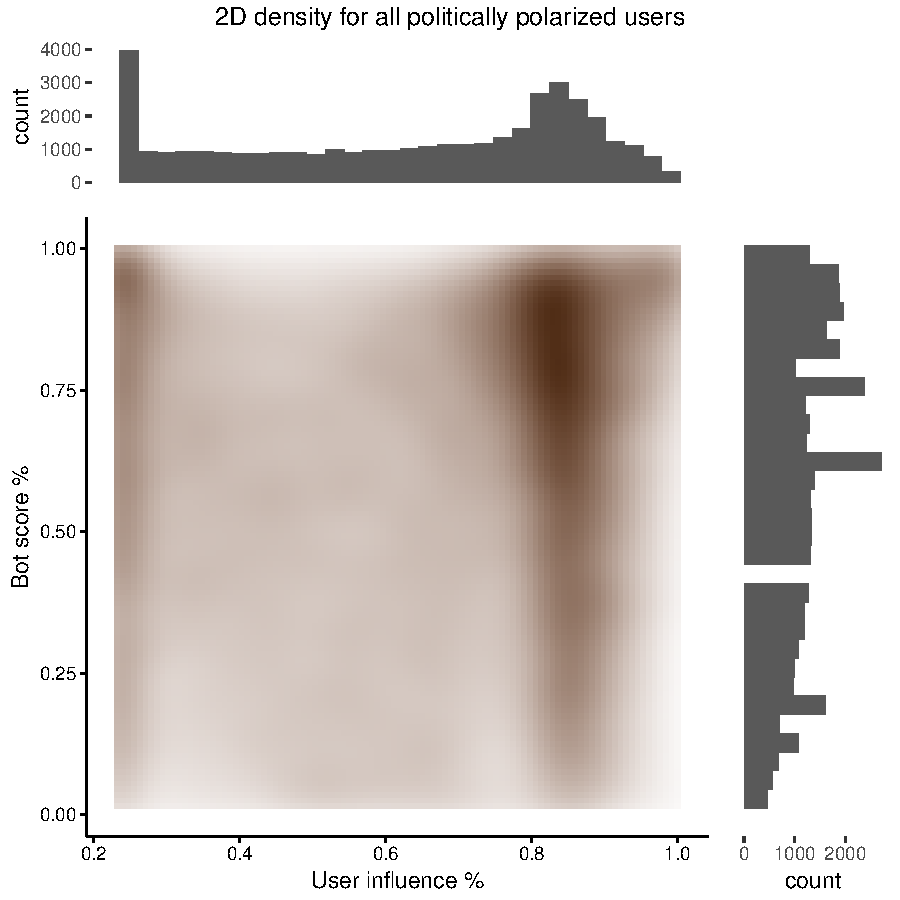
\includegraphics[width=\mywidth\textwidth, page=1]{2017-11-28-2d-density-map-influence-botscore}
	}
	\subfloat[] {
		\includegraphics[width=\mywidth\textwidth, page=2]{2017-11-28-2d-density-map-influence-botscore}
	}
	\subfloat[] {
		\includegraphics[width=\mywidth\textwidth, page=3]{2017-11-28-2d-density-map-influence-botscore}
	}
	\caption{
		2D density plots for all politically polarized users in \debate \textbf{(a)}, for Democrat users \textbf{(b)} and for Republican users \textbf{(c)}.
	}
	\label{si-fig:additional-2d}
%	\captionmoveup
\end{figure*}

\section{Generation of synthetic data}
\label{si-sec:generation-artificial}

This section completes and details the results concerning the evaluation on synthetic data, presented in the main text Sec.~\ref{subsec:ground-truth}.
This section details the construction of a synthetic random social graph (Sec.~\ref{si-subsec:random-graph}) and the sampling of synthetic cascades (Sec.~\ref{si-subsec:random-sampling}).
The purpose is to construct a synthetic dataset of cascades, in which the user influence ground truth is known.
Both the graph and cascade generators described here below reproduce closely the synthetic experimental setup described in~\cite{Du2013}.

\subsection{Generation of random graphs}
\label{si-subsec:random-graph}

In this section, we describe the construction of a synthetic social graph, with $n$ nodes, specified by its adjacency matrix $M$.
Each node corresponds to a synthetic user, and the edges correspond to synthetic follow relations.
We follow the below steps:
\begin{itemize}
	\item Given the number of nodes $n$ in the graph (here $1000$), create an null (all zero) adjacency matrix $M$ of size $n \times n$;
	\item Randomly choose the number of edges $|E|$, between $n/2$ to $n^2$.
	\item Randomly choose $i$ and $j$ between $1$ to $n$ and set $M_{ij}$ to $1$. Iterate this step until $|E|$ different edges are generated.
	\item The adjacency matrix $M$ defines the final random graph.
\end{itemize}

\subsection{Sampling synthetic cascades}
\label{si-subsec:random-sampling}

In this section we describe how to construct synthetic cascades, given a synthetic social graph $G$ constructed as shown in Sec.~\ref{si-subsec:random-graph}.
To generate one cascades, to each edge in $G$ we associate an exponentially distributed waiting time and we construct a shortest path tree.
We detail this procedure in the following steps:

\begin{itemize}
	\item Similar to previous work (ConTinEst~\cite{Du2013}), for each edge $\{v_i, v_j\} \in G$ draw a transmission rate $r_{ij}$ from a Weibull distribution of shape $k = 2$.
	\item Given the transmission rate $r_{ij}$, we draw an Exponentially distributed waiting time $\tau_{ij}$ using the inverse transform sampling:
		$$\tau_{ij} = -\frac{ln(s)}{r_{ij}}$$  
	where $s$ is draw uniformly from $U(0,1)$.
	\item Set $\tau_{ij}$ as the weight of edge $\{v_i, v_j\}$.
	\item Starting from a source node $v_s$, construct the shortest path tree from $v_s$ to all the other nodes in $G$;
	\item For each node $v_k$ compute two measures:
		$t_k$ -- its time of occurrence as the total waiting time along the path from $v_s$ to $v_k$ -- and
		$c_k$ -- the number of reachable nodes from $v_k$ in the shortest path tree;
	\item The generated cascade is $\{t_1,t_2,t_3 \cdots t_n\}$  where $(t_1 < t_2 < t_3 < \cdots t_n)$;
	\item The ground truth influence of node $v_k$ is the mean $c_k$ over multiple random graphs (here 100).
\end{itemize}

\section{Choosing the temporal decay parameter}
\label{si-sec:choose-temp-decay}

The temporal decay parameter $r$ shown in Eq.~\eqref{eq:prob-edge-mt} is determined by linear search. 
Eq.~\eqref{eq:prob-edge-mt} measures the probabilities of edges in the retweeting (diffusion) network, however the real diffusions are not observed.
We make the assumption that diffusions occur along edges in the underlying social graph (follower relation).
We measure the fitness of edge probability by the likelihood of uncovering the ground truth follower graph.
In other words, if the edge $\{v_i, v_j\}$ exists in the follower graph (i.e. $v_j$ is a follower of $v_i$) then the edge $\{v_i, v_j\}$  has the highest probability in the diffusion tree than the edge $\{v_l, v_j\}$ which does not exist in the following graph.
In other words, we are using the retweeting probability to predict the existence of edges in the social graph.
We randomly select 20 cascades, and we crawl the following list of every user appearing the the diffusions (the following list for a user $u_j$ consists of users $u_i$ followed by $u_j$).
We use this information as ground truth for the following prediction exercise:
given a user $u_j$ who emitted tweet $v_j$ in a particular cascade, we want to predict which among the users in the set $\{u_1, u_2, \ldots, u_{j-1}\}$ are followed by $u_j$.
Considering that $\mathds{P}(\{v_l, v_j\}). \forall l < j, j \geq 2$ are real numbers and the prediction target is binary, we use the AUC (are under ROC curve) the measure the prediction performance of a particular probability scoring function.
For each value of $r$ in Eq.~\eqref{eq:prob-edge-mt} we compute the mean AUC over all predictions.
We perform a linear search for the optimal $r$ between $10^{-8}$ to $3$. 
Finally, $6.2\times10^{-4}$ maximizes the mean of AUC and it is chosen as $r$ value in the experiments in Sec.~\ref{sec:evaluation-influence} and~\ref{sec:results-findings}.
%
%
% and using it over a cascade can generate a probabilistic retweeting network. 
%Nevertheless, the real retweeting network is unavailable so we use the friend network as the ground truth. Friends of a user on Twitter refer to users followed by him/her. That is, in a cascade a tweet A is from a tweet B if and only if the owner of B is 
%a friend of (followed by) the owner of A, which gives labels of edges .  By now, we have clarified probabilities and labels of edges in retweeting networks. As a choice to measure the performance of Eq. \ref{eq:prob-edge-mt}, AUC (Area Under Curve) is exploited in our experiments, which uses probabilities and labels of in-links of a node in the retweeting network. In other words, from the second tweet to the last one in a cascade, each owns a AUC calculated based on its in-links' probabilities and labels. We select 20 cascades to measure the performance and vary $r$ from $10^{-8}$ to $3$. Finally, $6.2\times10^{-4}$ maximizing the mean of AUC's is chosen as $r$.
%
%\TODO{MAR}{This is not clear! We need more details: 1) what is a friend in Twitter? 2) how many users were there in those 20 cascades 3) how do you use AUC, what probability do you use? 4) what is the domain of varying $r$ in the linear search?}

\section{Additional 2D densities plots}
\label{si-sec:polarization-map}

We show in Fig.~\ref{si-fig:additional-2d} the additional 2D density plots mentioned in the main text Sec.~\ref{subsec:user-influence-results}.

%\section{Content analysis of hashtags}
%\label{si-sec:hashtag-analysis}
%
%Content analysis~\cite{kimkuljis2010} was used to code the 1000 most frequently occurring hashtags according to their political polarity. More specifically, we used 
%Directed Content Analysis~\cite{hsieh-shannon-2005} to contextually analyse hashtags and code them according to their political polarity (or not, denoted as `neutral' and subsequently excluded from analysis). 
%This approach has been used in previous work to study hashtags on Twitter in a manner that is valid, reliable and replicable~\cite{small-2011}. 
%There were two previous studies of Twitter activity during the 2016 US presidential election that informed the development of our coding schema. 
%Firstly, \citet{FM7090} devised a binary classification scheme that attributed political partisanship to a small set of key hashtags as either `Trump-supporting' (\#donaldtrump, \#trump2016, \#neverhillary, \#trumppence16, \#trump) or `Clinton-supporting' (\#hillaryclinton, \#imwithher, \#nevertrump, \#hillary). 
%Secondly, in studying Twitter activity during the 1st US presidential debate~\cite{Kollanyi.2016.presidentialdebate} developed a coding schema that categorized tweets into seven categories based on the hashtags that occurred within the tweet. 
%However, the authors found that three `exclusive' categories (`Pro-Trump', `Pro-Clinton', and `Neutral') accounted for the majority (88.5\%) of observations. 
%
%Given the findings of previous research, we developed a code book with three categories: `Pro-Trump', `Pro-Clinton', and `Neutral'. 
%To ensure that hashtags were analysed within context, our content analysis methodology focussed on three units of analysis (following the approach developed by~\citet{small-2011}). 
%The first is hashtags, comprised of a set of the 1000 most frequently occurring hashtags over all tweets in our dataset. 
%The second unit of analysis was individual tweets that contained these hashtags. 
%In order to gain a more nuanced and `situated' interpretation of hashtag usage, for each hashtag we referred to a small random sample of tweets in our dataset that contained each given hashtag. 
%In some instances the polarity (or neutrality) was clear and/or already determined from previous studies, which helped to speed up the analysis of tweets. 
%The third unit of analysis was user profiles, which we referred to in situations where the polarity or neutrality of a given hashtag was unclear from the context of tweet analysis. 
%For example, \#partyoflincoln was used by both Republican and Democrat Twitter users, but an analysis of both tweets and user profiles indicated that this hashtag was \textit{predominantly} used by Pro-Trump supporters to positively align the Republican Party with the renowned historical figure of President Abraham Lincoln, who was a Republican. 
%The content analysis resulted in a subset of 93 pro-Democrat and 86 pro-Republican hashtags (a wordcloud visualization was given in Fig.~\ref{fig:wordclouds}), whilst the remaining `neutral' hashtags were subsequently excluded from further analysis.

\end{document}
